%==============================================================================
% Autorka: Bc. Eva Navrátilová
% Kontakt: xnavra54@stud.fit.vutbr.cz, navratie@gmail.com
%==============================================================================
% kodovani: UTF-8 (zmena prikazem iconv, recode nebo cstocs)
% encoding: UTF-8 (you can change it by command iconv, recode or cstocs)
%------------------------------------------------------------------------------
% zpracování / processing: make, make pdf, make clean
%==============================================================================
% Soubory, které je nutné upravit: / Files which have to be edited:
%   projekt-20-literatura-bibliography.bib - literatura / bibliography
%   projekt-01-kapitoly-chapters.tex - obsah práce / the thesis content
%   projekt-30-prilohy-appendices.tex - přílohy / appendices
%==============================================================================
%\documentclass[]{fitthesis} % bez zadání - pro začátek práce, aby nebyl problém s překladem
%\documentclass[english]{fitthesis} % without assignment - for the work start to avoid compilation problem
%\documentclass[zadani]{fitthesis} % odevzdani do wisu a/nebo tisk s barevnými odkazy - odkazy jsou barevné
%\documentclass[english,zadani]{fitthesis} % for submission to the IS FIT and/or print with color links - links are color
%\documentclass[zadani,print]{fitthesis} % pro černobílý tisk - odkazy jsou černé
%\documentclass[english,zadani,print]{fitthesis} % for the black and white print - links are black
\documentclass[zadani,cprint]{fitthesis} % pro barevný tisk - odkazy jsou černé, znak VUT barevný
%\documentclass[english,zadani,cprint]{fitthesis} % for the print - links are black, logo is color
% * Je-li práce psaná v anglickém jazyce, je zapotřebí u třídy použít 
%   parametr english následovně:
%   If thesis is written in english, it is necessary to use 
%   parameter english as follows:
%      \documentclass[english]{fitthesis}
% * Je-li práce psaná ve slovenském jazyce, je zapotřebí u třídy použít 
%   parametr slovak následovně:
%   If the work is written in the Slovak language, it is necessary 
%   to use parameter slovak as follows:
%      \documentclass[slovak]{fitthesis}
% * Je-li práce psaná v anglickém jazyce se slovenským abstraktem apod., 
%   je zapotřebí u třídy použít parametry english a enslovak následovně:
%   If the work is written in English with the Slovak abstract, etc., 
%   it is necessary to use parameters english and enslovak as follows:
%      \documentclass[english,enslovak]{fitthesis}

% Základní balíčky jsou dole v souboru šablony fitthesis.cls
% Basic packages are at the bottom of template file fitthesis.cls
% zde můžeme vložit vlastní balíčky / you can place own packages here

\usepackage{pgfplots}				% bar charts
\usepackage{enumitem,amssymb}		% enum with empty square
\usepackage{pgf-pie}				% pie charts
\usepackage{bchart}					% bar charts (pruhové grafy)
\usepackage{tikz}					% tikz pictures
\usepackage{siunitx}				% zarovnání v tabulce podle .

% Kompilace po částech (rychlejší, ale v náhledu nemusí být vše aktuální)
% Compilation piecewise (faster, but not all parts in preview will be up-to-date)
% \usepackage{subfiles}

% Nastavení cesty k obrázkům
% Setting of a path to the pictures
\graphicspath{{obrazky-figures/}{./obrazky-figures/}}
%\graphicspath{{obrazky-figures/}{../obrazky-figures/}}

%---rm---------------
\renewcommand{\rmdefault}{lmr}%zavede Latin Modern Roman jako rm / set Latin Modern Roman as rm
%---sf---------------
\renewcommand{\sfdefault}{qhv}%zavede TeX Gyre Heros jako sf
%---tt------------
\renewcommand{\ttdefault}{lmtt}% zavede Latin Modern tt jako tt

% vypne funkci šablony, která automaticky nahrazuje uvozovky,
% aby nebyly prováděny nevhodné náhrady v popisech API apod.
% disables function of the template which replaces quotation marks
% to avoid unnecessary replacements in the API descriptions etc.
\csdoublequotesoff

% =======================================================================
% balíček "hyperref" vytváří klikací odkazy v pdf, pokud tedy použijeme pdflatex
% problém je, že balíček hyperref musí být uveden jako poslední, takže nemůže
% být v šabloně
% "hyperref" package create clickable links in pdf if you are using pdflatex.
% Problem is that this package have to be introduced as the last one so it 
% can not be placed in the template file.
\ifWis
\ifx\pdfoutput\undefined % nejedeme pod pdflatexem / we are not using pdflatex
\else
  \usepackage{color}
  \usepackage[unicode,colorlinks,hyperindex,plainpages=false,pdftex]{hyperref}
  \definecolor{hrcolor-ref}{RGB}{223,52,30}
  \definecolor{hrcolor-cite}{HTML}{2F8F00}
  \definecolor{hrcolor-urls}{HTML}{092EAB}
  \hypersetup{
	linkcolor=hrcolor-ref,
	citecolor=hrcolor-cite,
	filecolor=magenta,
	urlcolor=hrcolor-urls
  }
  \def\pdfBorderAttrs{/Border [0 0 0] }  % bez okrajů kolem odkazů / without margins around links
  \pdfcompresslevel=9
\fi
\else % pro tisk budou odkazy, na které se dá klikat, černé / for the print clickable links will be black
\ifx\pdfoutput\undefined % nejedeme pod pdflatexem / we are not using pdflatex
\else
  \usepackage{color}
  \usepackage[unicode,colorlinks,hyperindex,plainpages=false,pdftex,urlcolor=black,linkcolor=black,citecolor=black]{hyperref}
  \definecolor{links}{rgb}{0,0,0}
  \definecolor{anchors}{rgb}{0,0,0}
  \def\AnchorColor{anchors}
  \def\LinkColor{links}
  \def\pdfBorderAttrs{/Border [0 0 0] } % bez okrajů kolem odkazů / without margins around links
  \pdfcompresslevel=9
\fi
\fi
% Řešení problému, kdy klikací odkazy na obrázky vedou za obrázek
% This solves the problems with links which leads after the picture
\usepackage[all]{hypcap}

% Informace o práci/projektu / Information about the thesis
%---------------------------------------------------------------------------
\projectinfo{
  %Prace / Thesis
  project={DP},            %typ práce BP/SP/DP/DR  / thesis type (SP = term project)
  year={2019},             % rok odevzdání / year of submission
  date=\today,             % datum odevzdání / submission date
  %Nazev prace / thesis title
  title.cs={Program pro interaktivní \\sestavování rodokmenů},  % název práce v češtině či slovenštině (dle zadání) / thesis title in czech language (according to assignment)
  title.en={Program for Interactive Family-Tree Making}, % název práce v angličtině / thesis title in english
  %title.length={14.5cm}, % nastavení délky bloku s titulkem pro úpravu zalomení řádku (lze definovat zde nebo níže) / setting the length of a block with a thesis title for adjusting a line break (can be defined here or below)
  %Autor / Author
  author.name={Eva},   % jméno autora / author name
  author.surname={Navrátilová},   % příjmení autora / author surname 
  author.title.p={Bc.}, % titul před jménem (nepovinné) / title before the name (optional)
  %Ustav / Department
  department={UITS}, % doplňte příslušnou zkratku dle ústavu na zadání: UPSY/UIFS/UITS/UPGM / fill in appropriate abbreviation of the department according to assignment: UPSY/UIFS/UITS/UPGM
  % Školitel / supervisor
  supervisor.name={Jaroslav},   % jméno školitele / supervisor name 
  supervisor.surname={Rozman},   % příjmení školitele / supervisor surname
  supervisor.title.p={Ing.},   %titul před jménem (nepovinné) / title before the name (optional)
  supervisor.title.a={Ph.D.},    %titul za jménem (nepovinné) / title after the name (optional)
  % Klíčová slova / keywords
  keywords.cs={Softwarové inženýrství, genealogie, rodokmen, GEDCOM, C++, Qt, uživatelské rozhraní}, % klíčová slova v českém či slovenském jazyce / keywords in czech or slovak language
  keywords.en={Software engineering, genealogy, family tree, GEDCOM, C++, Qt, user interface}, % klíčová slova v anglickém jazyce / keywords in english
  % Abstrakt / Abstract
  abstract.cs={Tato práce popisuje návrh a~implementaci aplikace pro interaktivní sestavování rodokmenů. Vyvinutá aplikace uživatelům umožňuje importovat a~exportovat genealogická data ve formátu GEDCOM, tato data dále upravovat a~zobrazovat a~exportovat rodové diagramy. Program je navržen s~důrazem na modularitu. Aplikace je implemetována v~jazyce C++ za využití frameworku Qt. Program byl otestován uživateli z~řad českých a~slovenských genealogů a~byl proveden a vyhodnocen průzkum jejich spokojenosti s~aplikací.}, % abstrakt v českém či slovenském jazyce / abstract in czech or slovak language
  % Jaký problém se řeší? Jaké řešení práce nabízí? Jaké jsou přesně výsledky? Jaký je jejich význam?
  abstract.en={This thesis describes the design and implementation of an application for interactive family-tree making. The application supports importing and exporting data in GEDCOM format, further editing of the data, visualizing the data in family charts and their export. The design of the program is modular. It is implemented using C++ and Qt. The program was released for testing amongst the group of Czech and Slovak genealogists and their opinions on the program were obtained and analysed.}, % abstrakt v anglickém jazyce / abstract in english
  % Prohlášení (u anglicky psané práce anglicky, u slovensky psané práce slovensky) / Declaration (for thesis in english should be in english)
  declaration={Prohlašuji, že jsem tuto diplomovou práci vypracovala samostatně pod vedením pana Ing. Jaroslava Rozmana, Ph.D. 
  Uvedla jsem všechny literární prameny a~publikace, ze kterých jsem čerpala.},
  % Poděkování (nepovinné, nejlépe v jazyce práce) / Acknowledgement (optional, ideally in the language of the thesis)
  acknowledgment={Děkuji vedoucímu své práce, panu Ing. Jaroslavu Rozmanovi, PhD., za cenné rady a~postřehy při konzultacích. Děkuji také členům facebookové skupiny Genealogie CZ+SK, kteří se účastnili průzkumu mezi uživateli a~ochotně se podíleli na testování aplikace.},
  % Rozšířený abstrakt (cca 3 normostrany) - lze definovat zde nebo níže / Extended abstract (approximately 3 standard pages) - can be defined here or below
  %extendedabstract={Do tohoto odstavce bude zapsán rozšířený výtah (abstrakt) práce v českém (slovenském) jazyce.},
  faculty={FIT}, % FIT/FEKT/FSI/FA/FCH/FP/FAST/FAVU/USI/DEF
  faculty.cs={Fakulta informačních technologií}, % Fakulta v češtině - pro využití této položky výše zvolte fakultu DEF / Faculty in Czech - for use of this entry select DEF above
  faculty.en={Faculty of Information Technology}, % Fakulta v angličtině - pro využití této položky výše zvolte fakultu DEF / Faculty in English - for use of this entry select DEF above
  %department.cs={Ústav matematiky}, % Ústav v češtině - pro využití této položky výše zvolte ústav DEF nebo jej zakomentujte / Department in Czech - for use of this entry select DEF above or comment it out
  %department.en={Institute of Mathematics} % Ústav v angličtině - pro využití této položky výše zvolte ústav DEF nebo jej zakomentujte / Department in English - for use of this entry select DEF above or comment it out
}

% Rozšířený abstrakt (cca 3 normostrany) - lze definovat zde nebo výše / Extended abstract (approximately 3 standard pages) - can be defined here or above
%\extendedabstract{Do tohoto odstavce bude zapsán výtah (abstrakt) práce v českém (slovenském) jazyce.}

% nastavení délky bloku s titulkem pro úpravu zalomení řádku - lze definovat zde nebo výše / setting the length of a block with a thesis title for adjusting a line break - can be defined here or above
%\titlelength{14.5cm}


% řeší první/poslední řádek odstavce na předchozí/následující stránce
% solves first/last row of the paragraph on the previous/next page
\clubpenalty=10000
\widowpenalty=10000

% checklist
\newlist{checklist}{itemize}{1}
\setlist[checklist]{label=$\square$}

\begin{document}
  % Vysazeni titulnich stran / Typesetting of the title pages
  % ----------------------------------------------
  \maketitle
  % Obsah
  % ----------------------------------------------
  \setlength{\parskip}{0pt}

  {\hypersetup{hidelinks}\tableofcontents}
  
  % Seznam obrazku a tabulek (pokud prace obsahuje velke mnozstvi obrazku, tak se to hodi)
  % List of figures and list of tables (if the thesis contains a lot of pictures, it is good)
  \ifczech
    \renewcommand\listfigurename{Seznam obrázků}
  \fi
  \ifslovak
    \renewcommand\listfigurename{Zoznam obrázkov}
  \fi
  % \listoffigures
  
  \ifczech
    \renewcommand\listtablename{Seznam tabulek}
  \fi
  \ifslovak
    \renewcommand\listtablename{Zoznam tabuliek}
  \fi
  % \listoftables 

  \ifODSAZ
    \setlength{\parskip}{0.5\bigskipamount}
  \else
    \setlength{\parskip}{0pt}
  \fi

  % vynechani stranky v oboustrannem rezimu
  % Skip the page in the two-sided mode
  \iftwoside
    \cleardoublepage
  \fi

  % Text prace / Thesis text
  % ----------------------------------------------
  %===============================================================================
% Autorka: Bc. Eva Navrátilová
% Kontakt: xnavra54@stud.fit.vutbr.cz, navratie@gmail.com
%===============================================================================

%===============================================================================
% ÚVOD
%===============================================================================

\chapter{Úvod}

 Sestavování rodinného rodokmenu je v~dnešní době módním trendem. Díky dostupnosti digitalizovaných historických pramenů se tomuto koníčku navíc může věnovat téměř každý. Není tedy divu, že genealogie jako obor v~posledních desetiletích zaznamenává nevídanou popularitu mezi širokou veřejností. \par
 V~dnešní době převážná část genealogů používá pro správu vypátraných dat počítačové programy. Těch je k~dispozici celá řada, od jednoduchých řešení dostupných zdarma až po komplexní placené aplikace, které uživatelům nabízejí shody s~rodokmeny jiných uživatelů. Výběr těchto programů je prozkoumán a~zhodnocen v~kapitole~\ref{chap:analyza}.\par
 Tato práce se věnuje právě specifikaci požadavků, návrhu a~implementaci interaktivní aplikace pro sestavování rodokmenů. Aby si tento program vydobyl své místo mezi již existujícími aplikacemi, došlo k~provedení průzkum mezi respondenty z~řad českých a~slovenských genealogů. Podněty, získané z~průzkumu, pak jsou posléze použity k~návrhu nové genealogické aplikace, který je rozebrán v~kapitole~\ref{chap:design}.\par
 Návrh aplikace sestává ze tří kroků. V~první řadě je třeba definovat rozšíření zastaralého standardu GEDCOM, používaného pro ukládání genealogických dat. Poté je proveden návrh jádra aplikace a~jeho rozhraní. Následuje už návrh samotného grafického uživatelského rozhraní aplikace.\par
 Kapitola~\ref{chap:implem} popisuje proces implementace programu. Obsahuje informace o~zvoleném implementačním jazyce, použitém frameworku a~jeho důležitých aspektech, použitých v~rámci vývoje. K~dispozici jsou zde i~náhledy hlavních součástí rozhraní výsledné aplikace. Nechybí ani metriky kódu.\par
 V~kapitole~\ref{chap:test} je shrnut průběh testování aplikace. Na jeho poslední etapě se podíleli samotní uživatelé z~řad českých a~slovenských genealogů. Jejich zpětná vazba je následně použita pro definici dalšího možného směru vývoje aplikace.\par 

%===============================================================================
% Genealogie
%===============================================================================

\chapter{Genealogie}
\label{chap:gene}
Genealogie je pomocná věda historická, která se zabývá vztahy mezi lidskými jedinci, přičemž tyto vztahy jsou dány jejich rodovým původem nebo příbuzenstvím. Spadá do ní také studium důsledků, které z~těchto vztahů vyplývají -- od historických až po sociální a~biologické. \par
Název této pomocné vědy historické pochází z~řeckého slova \emph{génos} (latinsky genus), tedy rod. Prakticky ve všech jazycích je název této vědy odvozen od stejného základu, výjimky tvoří jen němčina a~čeština se slovem rodopis. \par
Tradičně se genealogové zabývají studiem význačných rodů a~jedinců, které podrobují analýze z~hlediska jejich poměrů rodinných, třídních a~společenských. Zkoumáním větších souborů osob nebo vzorku typických představitelů určité třídní nebo sociální skupiny se genealogie snaží o~zobecnění některých problémů. Genealog může zkoumat předky určité osoby, ale také její potomky. \par
Samostatné úkoly oboru posléze spočívají v~tom, že genealogie rekonstruuje zasuté rodinné vazby a~vztahy, klade důraz na jejich dlouhodobý trend a~zjišťuje obecnější aspekty průběhu a~modifikací těchto vazeb. K~plnému proniknutí vlastní látky je zapotřebí nejen důkladných znalostí pramenné základny, ale i~značných vědomostí historických~\cite{bib:GeneVade}. \par

	\section*{Základní genealogické pojmy}
	\begin{description}[align=left] % labelwidth=4cm
		\item [Proband] neboli střen je osoba, od které odvíjíme rodové vztahy. Z~pohledu tvorby rodokmenu je to důležitý člověk, jelikož u~něj vždy začínáme rodopisné pátrání a~vykreslujeme rodopisné diagramy.
		\item [Generace] je určena jedním porodem vedoucím ke vzniku nového vztahu~\cite{bib:GeneRodoPojmy}. 
		\item [Pokrevenství] je termín označující osoby, pocházející od společného předka~\cite{bib:GeneVade}.
		\item [Stupeň pokrevenství] označuje blízkost příbuznosti mezi osobami. Počítá se podle generací, tedy podle počtu porodů, který osoby odděluje. Např. příbuzenství syna s~matkou je prvního stupně, je mezi nimi rozdíl jedné generace, protože ke vzniku příbuzenství stačilo jen aby matka syna porodila. Příbuzenství vnučky k~jejímu dědečkovi je druhého stupně, jsou mezi nimi dvě generace a~byly třeba dva porody, aby vztah vzniknul.
		\item [Přímá linie] je příbuzenské spojení mezi přímými předky a~potomky, tedy ve vztahu rodič – dítě. Přímá linie nespojuje jen dva předky, táhne se do nekonečna. Podle směru rozlišujeme, jestli je to vzestupná ascendentní linie, nebo sestupná descendentní linie. Ascendenti jsou předci, descendenti jsou potomci.
		\item [Pobočná linie] je každé nepřímé (nerodičovské) spojení mezi pokrevními příbuznými. Kříží přímou linii a~vytváří vztahy sourozenců, strýců a~tet se synovci a~neteřemi nebo bratranců a~sestřenic~\cite{bib:GeneRodoPojmy}.
	\end{description}

	\section*{Genealogická schémata}
	Základním cílem genealogického bádání je sestavení rodové posloupnosti. Tuto posloupnost je poté vhodné zobrazit v~určitém diagramu. Bývá zvykem zobrazovat mužské předky symbolem čtverce, ženy symbolem kruhu.
		\subsection*{Vývod}
		Vývod je nejpoužívanější forma genealogické tabulky, respektive způsob genealogického bádání. Vývod je příbuzenská posloupnost, registrující přímé předky určité osoby, kterou nazýváme proband. Při jeho vytváření se postupuje zpět do minulosti po všech jeho liniích, a~to jak mužských, tak i~ženských. Počet osob v~každé generaci se dá vyjádřit jako 
		\[ A_n = 2^{n-1} \]
		kde \(n = 1, 2, 3, ...\) udává číslo generace, přičemž proband je první generace~\cite{bib:GeneZakl}. \par
		Vývod bývá v~současnosti často zobrazován v~podobě stromu, kdy výchozí osoba bývá umístěna u~jeho kořenů a~její předci se od ní rozvíjejí do koruny. V~případě, že byly ve farnostech, kde je vývod zpracováván, pečlivě vedeny a~uchovávány matriční knihy, je možné ho vypracovat až do 17.století. Pokud jsou k~dispozici další archivní zdroje, je možné některé linie dovést ještě hlouběji do minulosti. Pravděpodobnost úspěchu bádání závisí především na existenci a~dostupnosti archivních fondů~\cite{bib:GeneTypyRodo}. \par
		\begin{figure}[H]
			\centering
			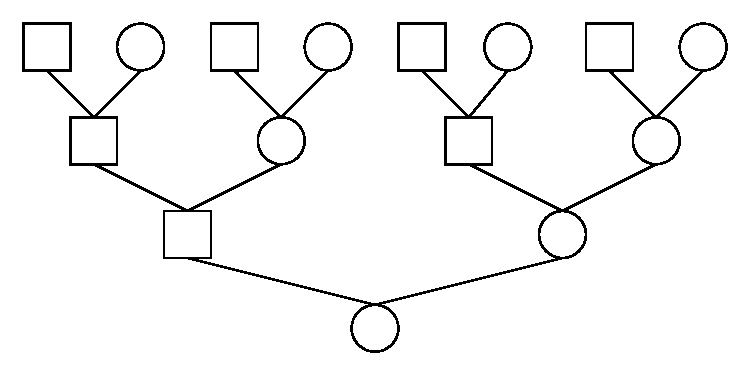
\includegraphics[width=9cm]{vyvod.pdf}
			\caption{Vývod z~osmi předků}
			%\label{fig:gene-vyvod}
		\end{figure}
		\begin{description}
			\item [Agnátní vývod] čili otcovská linie je redukovanou variantou vývodu sledující vždy pouze přímou hlavní linii, tzn. střen, otec, děd, praděd s~manželkami.  \par
			\item [Kognátní vývod] neboli mateřská linie je redukovanou variantou vývodu, která rozvíjí předky pouze v~ženské linii, tzn. střen, matka, bába, prabába a~jejich manželé~\cite{bib:GeneTypyRodo}.
		\end{description}
		\subsection*{Rozrod}
		Rozrod je příbuzenská posloupnost, přinášející potomky určitého manželského páru. Obsahuje tedy všechny osoby, které mají společného výchozího předka. Tím se rozrod blíží biologické představě o~potomstvu, protože eviduje veškeré potomstvo. Omezení spočívá jen v~tom, že se mezi potomky nejčastěji zaznamenávají pouze manželské děti~\cite{bib:GeneZakl}. \par
		Existují dva způsoby vytváření rozrodu. Prvním je sledování jednoho příjmení, strom v~takovém případě zahrnuje pouze potomky synů nebo nemanželské potomky dcer. Druhou variantou je sledování potomků synů i~dcer, bez ohledu na příjmení.  \par
		Rozrod poskytuje přehled o~genealogických vazbách v~rámci rodu. Jeho zpracování je časově velmi náročné, může totiž zahrnovat několik tisíc osob~\cite{bib:GeneTypyRodo}.
		
	\section*{Genealogické prameny}
	Hlavními prameny genealogických studií jsou především písemnosti diplomatického rázu. Významné místo mezi nimi mají zpočátku, tj. z~doby před soustavnou evidencí obyvatelstva, různé úřední a~veřejné knihy. Od 16. století jsou to zejména matriky, hlavně církevní, i~když ty jsou ve větší úplnosti dochovány až od 18. století. Původně jsou jen velmi všeobecné, posléze však přinášejí vedle informací o~narození a~o~rodičích i~údaje svatební a~úmrtní a~v~průběhu doby se také v~tomto smyslu specializují~\cite{bib:GeneVade}. Náhled zápisu v~matrice je k~dispozici v~obrázku \ref{fig:matrica}.\par
	\begin{figure}[H]
		\centering
		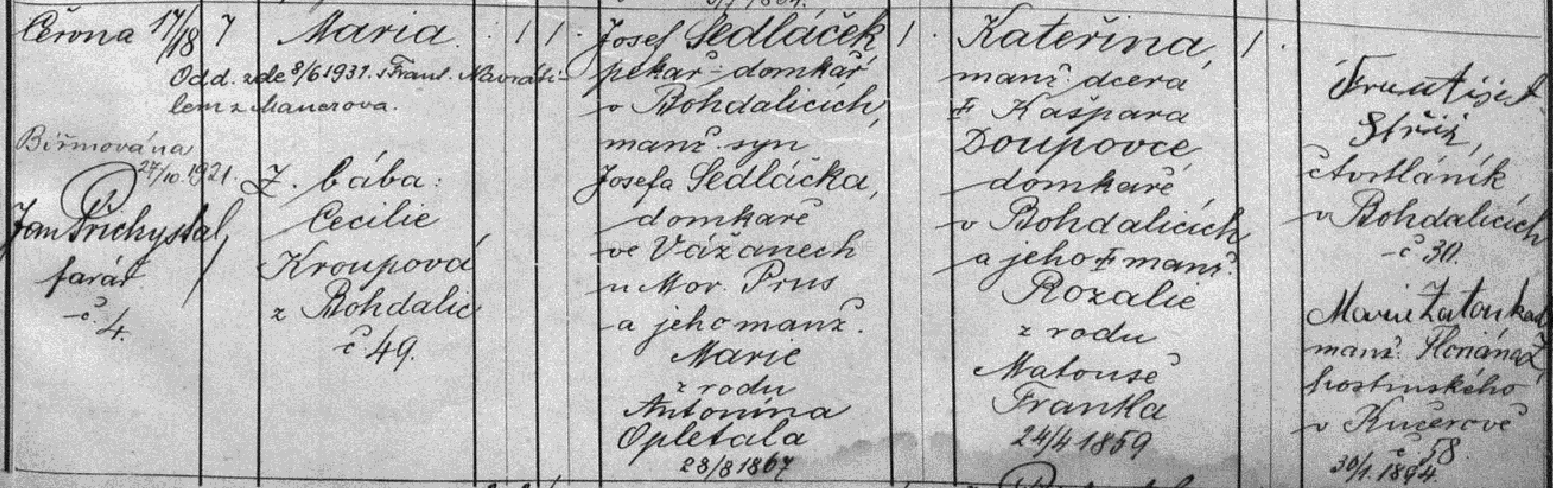
\includegraphics[width=15cm]{matrika.png}
		\caption{Příklad matričního zápisu o~narození z~roku 1905 (převzato z~\cite{bib:GeneActaPublica})}
		\label{fig:matrica}
	\end{figure}
	Archivů, kde je možné bádat v~základním prameni pro rodopisce, tedy v~matrikách, je v~České republice devět. Jedná se o~takzvané oblastní nebo zemské archivy, eventuálně archiv města v~případě Prahy. Státní oblastní archivy se nacházejí v~Praze, Litoměřicích, Plzni, Třeboni a~Zámrsku, zemské archivy pak v~Brně a~Opavě. V~těchto archivech se nacházejí křesťanské matriky, židovské najdeme v~Národním archivu v~Praze. \par
	Všechny archivy mají v~současnosti matriky zveřejněné na internetu. Buď se jedná o~část matrik, což je případ většiny archivů (stav v~roce 2012), nebo o~kompletní matriční sbírku, což je případ archivu v~Třeboni~\cite{bib:GeneLedni}. K~pátrání tedy ve většině případů není potřeba nic víc než počítač s~připojením k~internetu. Po svých předcích díky tomu může pátrat téměř každý. \par	


	% Standard GEDCOM

	\section{Standard GEDCOM}
	\label{sec:gedcom}
	GEDCOM je definice formátu pro ukládání a~výměnu genealogických dat. Jedná se o~nejrozšířenější \emph{de facto} standard~\cite{bib:GedcomGeniStd} pro ukládání genealogických dat, který je podporovaný většinou genealogických programů.\par
	Tento formát byl vyvinut Církví Ježíše Krista Svatých posledních dnů a~jeho cílem bylo poskytnout flexibilní jednotný formát pro výměnu digitálních genealogických dat. Název formátu vznikl jako akronym anglického slovního spojení \emph{GEnealogical Data COMmunications} -- sdílení genealogických dat~\cite{bib:Gedcom551Spec}.\par
	Soubory ve formátu GEDCOM sestávají z~prostého textu, v~němž jsou prostřednictvím definovaných struktur zaznamenána data o~jednotlivých osobách a~jejich rodinných svazcích. Soubory vyhovující tomuto standardu mají příponu \texttt{.ged}.

		\subsection*{Historie standardu GEDCOM}
		První verze formátu GEDCOM, která byla ustavena coby standard, byla v~říjnu roku 1987 verze 3.0. Verze~1 a~2 byly pouze koncepty, jejichž cílem bylo především vzbudit veřejnou diskuzi. V~srpnu roku 1989 pak byla vydána verze 4.0. \par
		Série konceptů 5.x podporuje základní struktury představené ve verzi 3.0, a~obohacuje je o~četná rozšíření. V~roce 1996 vznikla aktuální verze formátu označovaná jako standard 5.5. Od vydání poslední verze formátu v~roce 2002 se zdá, že vývoj tradičního GEDCOM formátu stagnuje. \par
		V~roce 2011 byl představen nový formát GEDCOM 6.0, známější pod názvem GEDCOM X, který naznačuje odklon od odkazu tradičního GEDCOM formátu a~poukazuje na jeho využití XML~\cite{bib:GedcomXOrig}. Formát přichází oproti výše zmíněným verzím se zcela novým pojetím problému sdílení genealogických dat. Soubory v~tomto formátu nesou příponu \texttt{.gedx}, a~obsahují komprimovaná data. Kromě XML souboru s~genealogickými daty, který má zcela jinou strukturu než původní GEDCOM soubory, zde také nalezneme veškerá multimediální data přiložená k~rodokmenu~\cite{bib:GedcomXHome}. \par
		
		\subsection*{Omezení standardu GEDCOM}
		%\label{subsec:OmezStd}
		Hlavním omezením standardu je jeho zastaralost a~zanedbání jeho aktualizací. K~roku 2019 je nejnovější formální specifikace tohoto formátu více než dvacet let stará. Za tuto dobu proběhl na poli genealogického pátrání velký technologický posun; jako příklad může posloužit třeba digitalizace archiválií, která je v~dnešní době velmi rozšířeným trendem. Je tedy zřejmé, že formát vytvořený na konci devadesátých let nemůže být schopen nově vzniklé potřeby spojené s~tímto vývojem naplnit. \par
		Další z~omezení standardu plyne z~jeho snahy o~flexibilitu. Návrh formátu je záměrně nedostatečně formálně specifikovaný, a~to proto, aby umožnil ukládaní celé řady rozličných dat v~různých kódováních. \par
		Formát také například umožňuje definici vlastních značek. Této skutečnosti využívají některé genealogické programy a~vzniká tak nespočet upravených verzí standardu. Tato skutečnost ve spojení s~nedostatečnou či neexistující dokumentací těchto upravených verzí standardu vede k~problémům při importování do jiných programů, kdy může docházet k~vynechávání některých dat~\cite{bib:GedcomNoSynch}. \par
		Na druhou stranu ale díky této skutečnosti formát dokázal přežít dvacetiletou periodu, kdy jeho oficiální vývoj ustrnul. Jeho flexibilita poskytuje v~současné době jedinou možnost, jak prostřednictvím formátu GEDCOM předávat data, s~nimiž oficiální definice formátu nepočítala. Nejedná se tedy o~omezení v~pravém slova smyslu, přestože působí na poli genealogických programů a~sdílení dat mezi nimi nemalé problémy. \par
		
		\subsection*{Struktura souboru dle standardu GEDCOM 5.5.1}
		V~následujících odstavcích bude popsána zjednodušená struktura souborů dle formátu GEDCOM. Bude použita symbolika definovaná v~dokumentu~\cite{bib:Gedcom551Spec} popisujícím standard a~budou zmíněny pouze ty náležitosti standardu, které byly využity v~navrhovaném programu. \par
		Soubor vyhovující standardu GEDCOM reprezentuje databázi genealogických dat formou sekvenčního toku souvisejících záznamů, přičemž na každém řádku je právě jeden záznam. \par
		Každý řádek souboru má pevně danou strukturu. Začíná povinným číslem identifikujícím hloubku zanoření ve struktuře formátu. Nejsvrchnější úroveň je označena číslicí 0, postupným zanořováním se hodnota zvyšuje. \par
		Za číselnou hodnotou následuje nepovinná reference, označující jedinečným identifikátorem aktuální strukturu. Identifikátor je složen z~alfanumerických znaků, obalených z~obou stran znakem zavináč. \par
		Nepovinná reference je následována povinnou značkou. Značka je složena z~alfanumerických znaků, přičemž písmena bývají obvykle velká. Značka svým standardizovaným tvarem určuje kontext dat uložených na daném řádku. \par
		Za značkou se může nacházet nepovinná sekce ukládající hodnotu. V~této části struktury bývají uložena konkrétní data v~textové podobě, případně reference na nějakou strukturu, nacházející se v~souboru. \par
		Tyto jednotlivé sekce jsou od sebe odloučeny prostřednictvím oddělovače, který je definován jako znak mezera. Každý řádek je potom zakončen povinným ukončovacím znakem, odpovídajícím novému řádku. \par
		
		\begin{verbatim}
			gedcom_line:= 
			level + [optional_xref_ID] + tag + [optional_line_value] + terminator
		\end{verbatim}
		
		Soubor samotný se strukturálně dělí na tři části. Sestává z~povinné hlavičky \texttt{HEADER}, libovolného počtu záznamů \texttt{RECORD} a~ukončující značky \texttt{TRLR}. \par
		Hlavička \texttt{HEADER} eviduje záznam o~kódování souboru, použité verzi formátu GEDCOM, zdrojovém a~cílovém programu, datu a~času exportu a~zaznamenává i~referenci na strukturu přispěvatele, který zaznamenal uložená data. \par
		Tělo souboru \texttt{RECORD} je prostorem, kde jsou uložena veškerá data o~osobách, jejich rodinných svazcích, zdrojích a~přispěvatelích. Obsahuje tedy všechna genealogická data. \par
		Záznamy o~osobách jsou určené značkou \texttt{INDI}. Každá osoba má přiřazený jedinečný identifikátor, skrze nějž je možné se na ni odkazovat z~jiných struktur v~souboru. Struktura \texttt{INDI} může obsahovat data o~jméně a~pohlaví osoby, a~podporuje také zanoření struktur popisujících životní události jako např. narození, křest či úmrtí. Dále je možné do záznamu o~osobě vnořit struktury pro zaznamenání atributů, mezi něž patří například struktura pro záznam bydliště, zaměstnání, nebo vzdělání osoby. U~osoby je také možné uložit záznam obsahující poznámky. V~novějších verzích formát GEDCOM umožňuje ukládat například i~informace o~e-mailové adrese či webové stránce. \par
		Další z~genealogického pohledu důležitou strukturou je struktura pro zaznamenávání rodinných vztahů \texttt{FAM}. I~tato struktura může mít přiřazen identifikátor. Hlavní objektivou této struktury je provazovat jednotlivě definované osoby rodinnými vztahy. Umožňuje definovat reference na osoby reprezentující partnera, partnerku a~jejich potomstvo. Záznam je validní i~v~případě, kdy jsou uvedeni jen někteří ze zmíněných aktérů -- např. pouze partnerka a~její děti, nebo pouze dva bezdětní partneři. Nechybí ani podpora vnoření záznamů o~událostech, kde v~tomto případě figurují především sňatek a~rozvod. \par
		Další záznam je určen značkou \texttt{SOUR} a~definuje zdroj. Opět může být opatřen identifikátorem. Skrze tuto strukturu lze definovat obecné informace o~zdroji a~dále je opatřit datovými oddíly, rozdělenými dle evidovaných událostí. Každý z~těchto oddílů může obsahovat další informace v~podobě datace či určení místa. Tyto zdroje je potom možné prostřednictvím reference citovat ve strukturách popisujících životní události u~osob a~rodin.\par
		Značka \texttt{SUBM} definuje záznam o~přispěvateli. Přispěvatel je osoba, která dodala genealogická data evidovaná v~souboru. Nejčastěji se tedy jedná o~genealoga vytvářejícího rodokmen. \par
		Za sekvencí se záznamy musí v~každém souboru GEDCOM následovat ukončovací značka \texttt{TRLR}. 
		
		
%===============================================================================
% Analýza existujících aplikací
%===============================================================================

\chapter{Analýza existujících řešení}
\label{chap:analyza}
	% Aplikace

	Pro příznivce genealogie je k~dispozici celá řada programů ke správě a~zobrazování genealogických dat. Řadí se mezi ně jak volně dostupný software, tak i~aplikace, které jsou placené. Tato sekce je zaměřena na zhodnocení vybraných genealogických aplikací, které jsou často používané v~české genealogické komunitě. \par
	Všechny aplikace byly testovány na tomtéž souboru reprezentativních dat, popisujících rodokmen Karla IV.~\cite{bib:ApliAnceHome}. Tato data byla též využita k~vytvoření všech níže prezentovaných snímků aplikací.\par

		\section{Ancestry}
		\label{sec:ance}
		Program Ancestry (před lety nazývaný Rodokmen) je český zdarma šířený genealogický databázový program, jehož autorem je Martin Doležal. Program umožňuje uživateli uložit si nejrůznější informace o~svých příbuzných, vytvářet mezi jednotlivými osobami příbuzenské vztahy, vkládat doplňující fotografie či jiné soubory. Součástí Ancestry jsou i~funkce na zobrazování, pomocí kterých je možné vygenerovat si příbuzenské stromy, jako je např. rodový vývod, rozrod rodu apod., libovolně si je v~programu upravovat a~dále uložit třeba jako JPG, PDF či SVG. \par
		Program nabízí i~celou řadu dalších funkcí, které se při práci s~genealogickými daty mohou hodit. Patří mezi ně např. zobrazování výročí, statistik, hledání příbuzenských vztahů mezi osobami, spojování dvou rodokmenů, kalkulačka dat, a~další. Samozřejmostí je podpora genealogického standardu GEDCOM 5.5.1 či například široce nastavitelný export do HTML stránek. \par
		Autor programu na svých stránkách uvádí, že chystá novou verzi aplikace, která bude fungovat i~na Linuxu. Po dobu několika let se ale k~této informaci již nevyjádřil, a~tak se zdá, že její vývoj stagnuje~\cite{bib:ApliAnceHome}. \par
		Program využívá vlastní formát pro ukládání dat, který je koncipován jako komprimované XML. Uložené soubory s~daty mají koncovku \texttt{.rodz}. \par
		Hlavní obrazovka aplikace slouží současně pro editaci základních údajů osoby. Není zde přímo zobrazen žádný rodinný strom, což může být pro nové uživatele matoucí. Na levé straně je obrazovka doplněna o~seznam evidovaných osob. \par
		Program Ancestry je skvělou volbou pro genealogy, kteří chtějí používat nekomplikovaný program s~jednoduchým rozhraním, kde je vše na dosah. Ancestry umožňuje zadávat většinu údajů o~osobě na jediné obrazovce a~šetří tím čas uživatele. Jednoduchost rozhraní je ale vykoupena tím, že uživatel neodstává takovou svobodu v~zadávání pokročilejších dat, jako jsou například odkazy na zdroje informací, záznam křtiteli či o~porodní bábě. Tento nedostatek lze ale do jisté míry kompenzovat prostřednictvím zaznamenání takových dat do pole pro poznámky. \par
		Vykreslení stromu je v~tomto programu graficky strohé, ale funkční. Uživatel si sám může zvolit, jaké informace a~jakým způsobem ve stromu zobrazit. Pozitivem je také možnost vykreslený strom dále upravovat např. posouváním či odstraňováním polí. \par
		\begin{figure}[H]
			\centering
			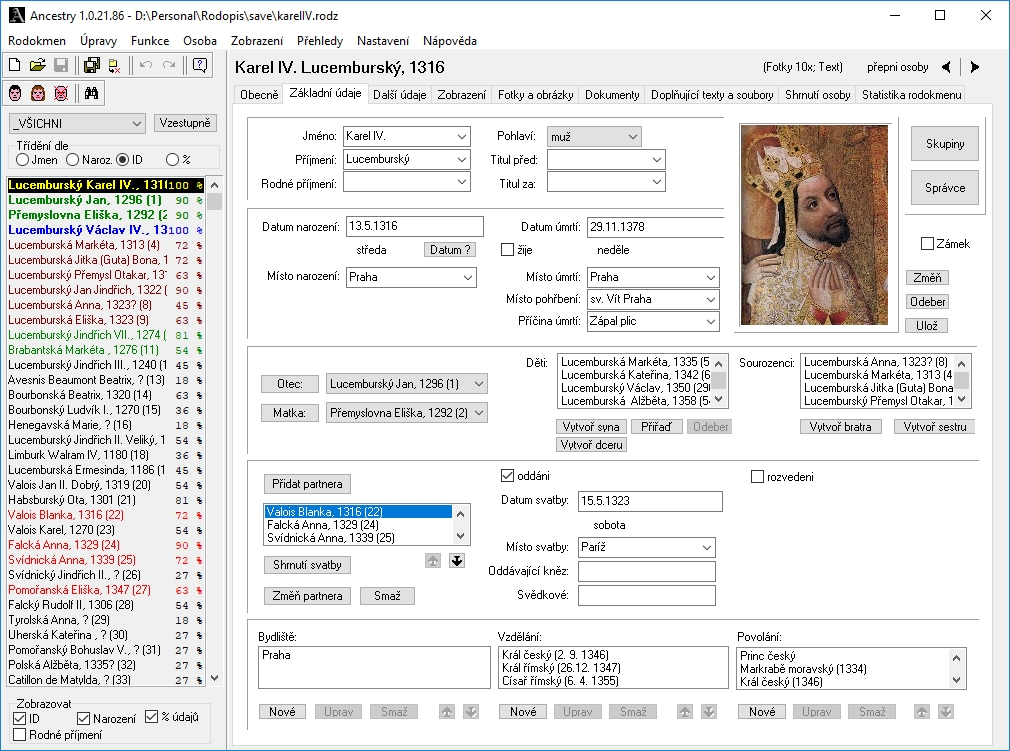
\includegraphics[width=15cm]{appAnce.jpg}
			\caption{Aplikace Ancestry}
			%\label{fig:appAnce}
		\end{figure}

		\section{Ahnenblatt}
		\label{sec:appAhnen}
		Ahnenblatt je německá zdarma dostupná genealogická aplikace, která je jednoduchá na používání a~je určena pro platformu Windows. Slouží ke správě genealogických dat a~umožňuje generovat působivé výkazy a~grafické stromy. Program nabízí celou řadu způsobů, jak importovat a~exportovat data, pro její uživatele je tedy jednoduché sdílet data s~ostatními. Ahnenblatt je k~dispozici v~celé řadě jazyků, mezi něž se řadí kromě angličtiny a~němčiny i~čeština~\cite{bib:ApliAhnenCom}. \par
		Program Ahnenblatt používá pro ukládání dat vlastní formát souborů, který používá koncovku \texttt{.ahn}. Aplikace ale podporuje i~import a~export dat ve formátu GEDCOM, umožňuje tedy sdílení dat s~ostatními aplikacemi. \par
		Hlavní obrazovka aplikace přehledně zobrazuje vybranou část rodokmenu, je tedy jednoduché se v~ní na první pohled zorientovat. I~navigace rodokmenem je díky této skutečnosti rychlá a~přehledná. \par
		Ahnenblatt umožňuje uživateli zadávat široké spektrum dat o~evidovaných osobách. Zadávání ale probíhá ve speciálním plovoucím okně, které je rozčleněné na záložky dle kategorií dat, viz obrázek~\ref{fig:appAhnen}. Tato skutečnost může být při zadávání většího množství dat pro uživatele rušivá. \par
		Na druhou stranu ale program vyniká ve vykreslování genealogických schémat. Dialog pro jejich vykreslování je sice velmi nepřehledný a~složitě členěný, nabízí ovšem zajímavé funkcionality. Je zde na výběr celá řada genealogických diagramů, které umožňují i~velké množství detailních nastavení. Uživatel si mimo jiné opět může vybrat data k~zobrazení, už ale nemůže ovlivnit jejich formát. Kromě toho pro diagramy existuje celá řada líbivých grafických šablon, jejichž zobrazení je možné si dále přizpůsobit, např, nastavením obrázku na pozadí. Zobrazení je též možné exportovat do celé řady formátů včetně PDF a~obrazových formátů. \par
		\begin{figure}[H]
			\centering
			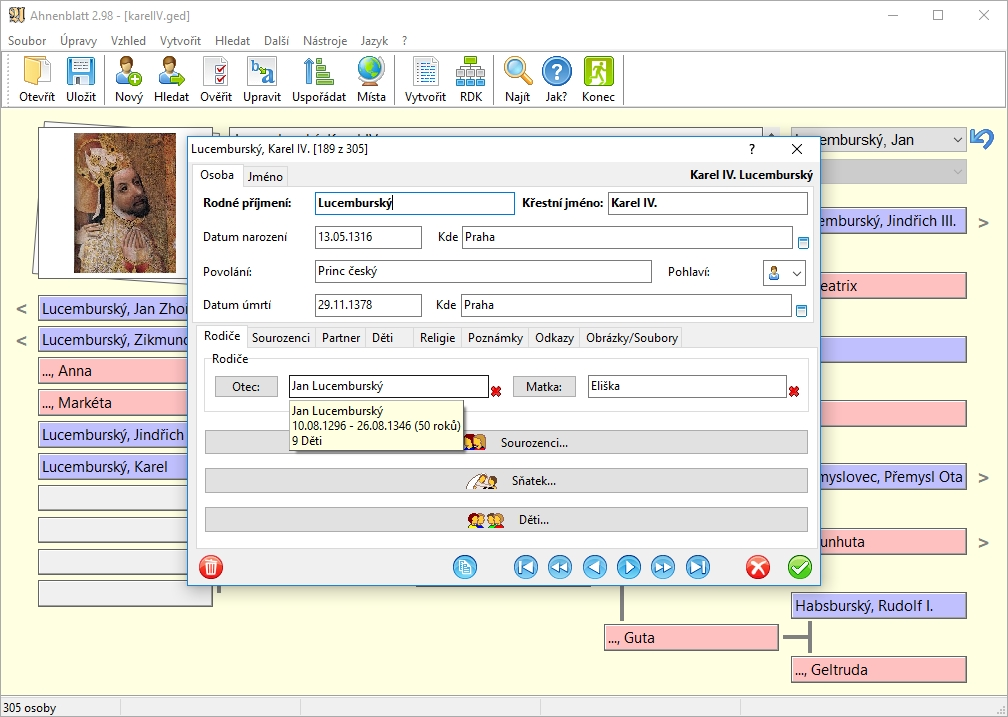
\includegraphics[width=15cm]{appAhnen.jpg}
			\caption{Aplikace Ahnenblatt}
			\label{fig:appAhnen}
		\end{figure}

		\section{MyHeritage}
		\label{ssec:myher}
		MyHeritage je internetová aplikace vytvořená společností MyHeritage Ltd. Společnost byla založena v~roce 2003 současným generálním ředitelem, podnikatelem a~rodinným historikem Giladem Japhetem. Od skromného garážového start-upu se MyHeritage rozrostla k~celosvětové společnosti s~95 milióny uživatelů z~celkem 196 zemí~\cite{bib:ApliMyHer}.\par
		Aplikace nabízí uživatelské rozhraní ve více než čtyřiceti jazycích. Základní verze aplikace je k~dispozici zdarma, je ovšem omezena počtem osob v~rodokmenu. Aplikace poté nabízí tři úrovně předplacených licencí, odstupňované dle rozšiřujících funkcionalit.\par
		Vyzkoušena byla verze aplikace zdarma. Aplikace umožňuje import dat ve formátu GEDCOM. Data jsou poté uchovávána v~rámci aplikace v~nespecifikovaném formátu. Uživatel má možnost data kdykoliv exportovat zpět do formátu GEDCOM.
		Na hlavní obrazovce je vykreslen rodokmen, v~němž je vycentrována aktuálně vybraná osoba. Detaily této osoby je též možné zobrazit v~levé části obrazovky.\par
		Při požadavku na editaci dat se otevře modální okno se všemi základními informacemi v~editovatelných polích. Při požadavku na editaci pokročilých dat je uživatel přesměrován na samostatnou stránku. Aplikace též podporuje přidávání zdrojů a~citací.\par
		Aplikace umožňuje vykreslení celé řady schémat. K~dispozici jsou i~graficky povedené šablony. Nastavení schémat, nabízená uživateli, jsou dostatečně rozsáhlá. Výsledné stromy jsou vizuálně pěkně zpracované. Diagramy je možné stáhnout ve formátu PDF, nebo objednat jejich tisk přímo u~společnosti MyHeritage.\par
		\begin{figure}[H]
			\centering
			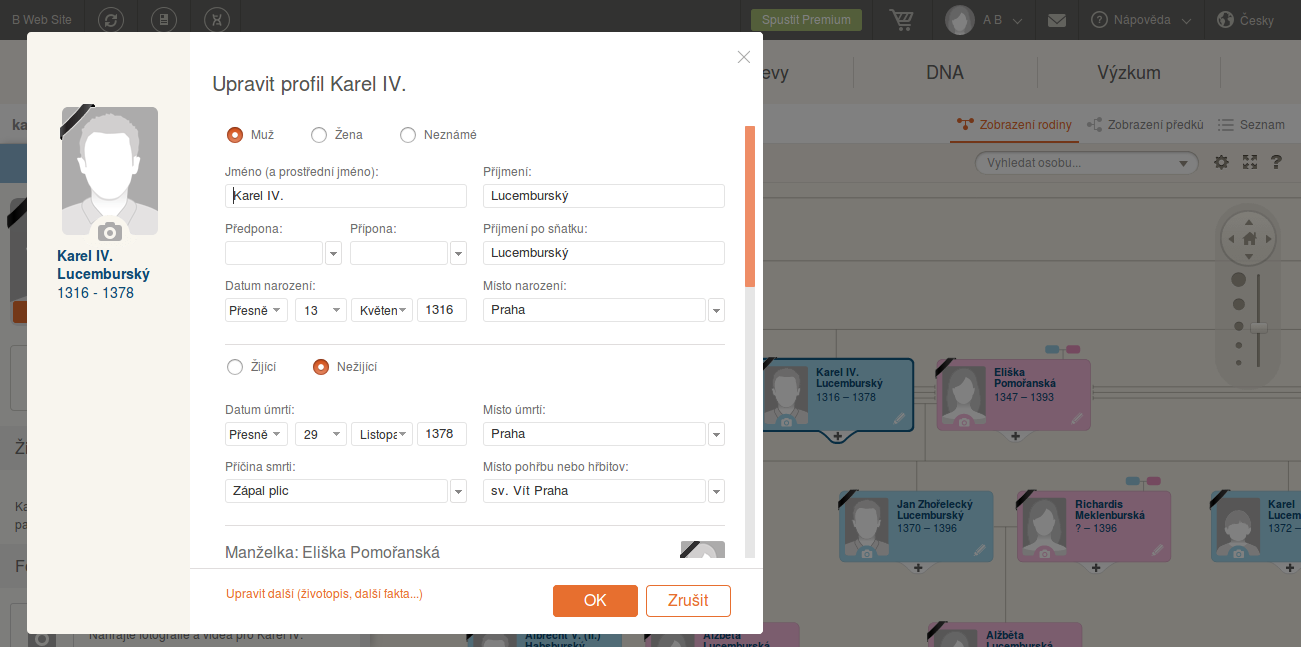
\includegraphics[width=15cm]{appMyHer.png}
			\caption{Aplikace MyHeritage}
			\label{fig:appMyHer}
		\end{figure}
		
		\section{Family Tree Builder}
		Family Tree Builder je desktopová aplikace vytvořená společností MyHeritage Ltd., jejíž využívání je podmíněno registrací na webových stránkách MyHeritage. Program podporuje čtyřicet jazyků uživatelského rozhraní, mezi nimiž nechybí ani čeština. Stejně jako internetová aplikace MyHeritage, popsaná v~sekci~\ref{ssec:myher}, je tato aplikace k~dispozici zdarma pouze s~omezenou funkcionalitou~\cite{bib:ApliFTB}. \par
		Vyzkoušena byla neplacená verze. Hlavním rysem této verze je omezený počet osob v~rodokmenu. Těch může být vytvořeno pouze dvě stě, dlouhodobí uživatelé bývají tedy nuceni si program předplatit. \par
		Aplikace plně spolupracuje s~formátem GEDCOM, který si ale transformuje do tzv. Genealogického projektu, který dostává příponu \texttt{.ftb} nebo \texttt{.zed}. 
		Hlavní obrazovka aplikace zobrazuje vybranou osobu a~její nejbližší rodinné příslušníky. Nalevo je navíc k~dispozici seznam všech zaznamenaných osob. \par
		Editace osob se provádí ve zvláštním okně. To se dále dělí na záložky dle kategorie editovatelných informací, které jsou v~nich obsaženy. V~jedné ze záložek je navíc možné zadávat detailní data o~zdrojích informací, což většina genealogických aplikací neumožňuje. \par
		Aplikace za ostatními nezaostává ani ve vykreslování genealogických schémat. Diagramů je k~dispozici celá řada a~jejich výsledné zobrazení je graficky velmi pěkně zpracované. Uživateli se opět naskýtá možnost vybírat z~několika stylů. Začínající genealogové také jistě ocení Průvodce diagramy, který popisuje jednotlivé typy diagramů a~naviguje uživatele procesem výběru toho správného. Diagram je poté možné z~aplikace exportovat do formátů PDF a~JPG. \par
		\begin{figure}[H]
			\centering
			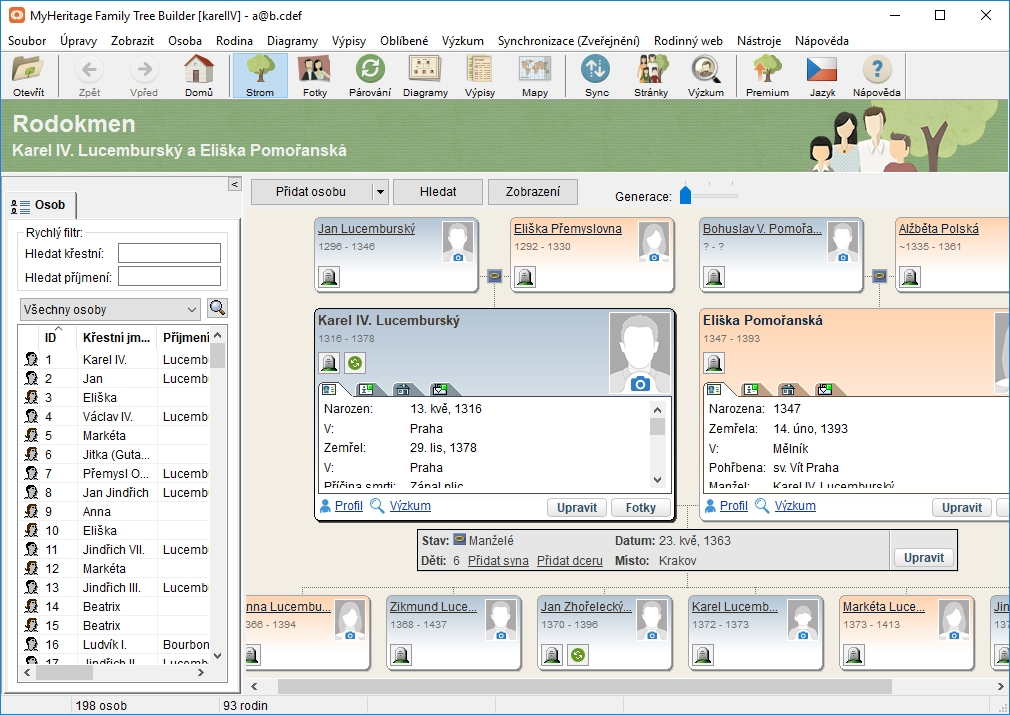
\includegraphics[width=15cm]{appFTB.jpg}
			\caption{Aplikace Family Tree Builder}
			\label{fig:appFTB}
		\end{figure}

		\section{RootsMagic Essentials}
		Firma RootsMagic nabízí již přes dvacet let celou řadu programů zaměřených na zpracovávání rodinné historie. Prvním z~jejich počinů byl program \emph{Family Origins}, dnes v~tradici pokračuje program \emph{RootsMagic}, který slouží k~zaznamenávání a~organizaci výsledků genealogického výzkumu a~umožňuje jeho jednoduché sdílení. Mezi další produkty firmy patří například aplikace pro podporu psaní rodinné kroniky, organizaci rodinných sjezdů, či sledování migrace předků~\cite{bib:ApliRoots}. \par
		Všechny aplikace produkované touto firmou jsou zpoplatněné, k~dispozici jsou ale i~verze zdarma, které postrádají část funkcionality. Vyzkoušena byla právě neplacená verze aplikace. \par
		Kromě importování a~exportování souboru ve formátu GEDCOM umožňuje aplikace import speciálních formátů používaných jinými aplikacemi. Upravená data potom program ukládá ve vlastním formátu s~koncovkou \texttt{.rmgc}. \par
		Hlavní obrazovka aplikace do jisté míry připomíná aplikaci Ahnenblatt zmíněnou v~kapitole~\ref{sec:appAhnen}. Je zde znázorněn vývod předků vybrané osoby, doplněn na levé straně seznamem všech evidovaných osob. Toto zobrazení umožňuje uživateli rychlou orientaci i~navigaci v~rodokmenu. \par
		Editace osoby je prováděna ve speciálním dialogu. Ten obsahuje seznam uložených informací a~nabízí uživateli celou řadu možností, jak je aktualizovat a~rozšířit. Pozitivem aplikace je možnost detailní evidence zdrojů informací. Celkové množství ovládacích prvků v~okně ovšem ohrožuje jeho přehlednost a~přidávání nových dat je nepříliš uživatelsky přívětivé a~velmi zdlouhavé. \par
		Grafické zpracování vývodu je v~aplikaci RootsMagic velmi minimalistické a~neumožňuje téměř žádná uživatelská nastavení. Rozrod a~pokročilejší diagramy není možné vygenerovat vůbec. Základní verze aplikace navíc vůbec neumožňuje uložení grafického výstupu, pouze jeho tisk. \par
		\begin{figure}[H]
			\centering
			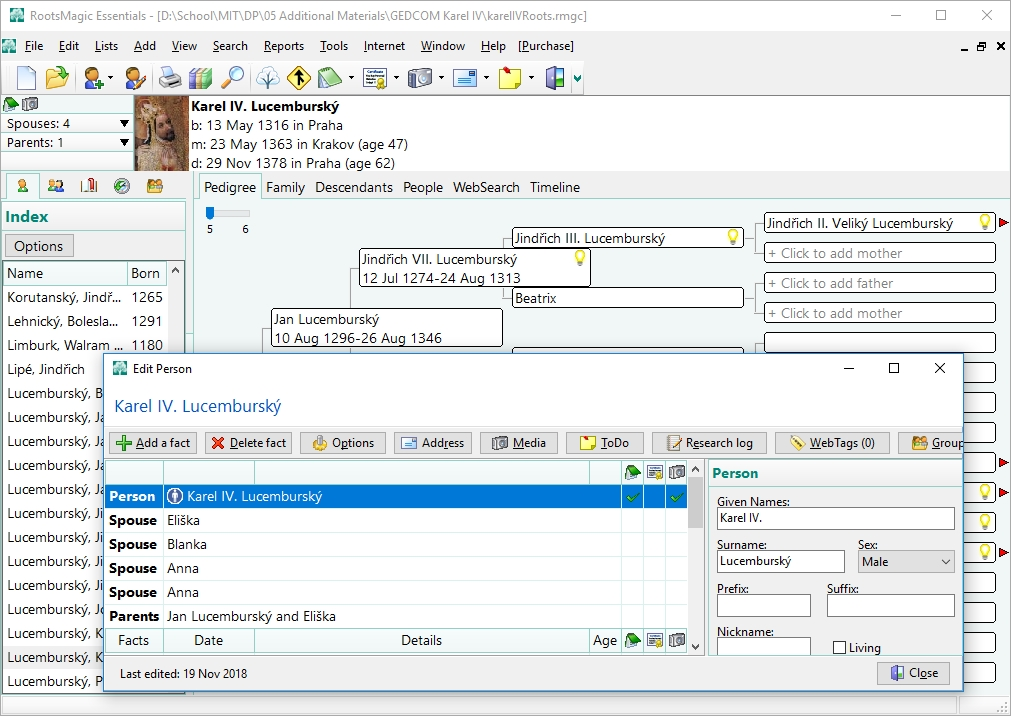
\includegraphics[width=15cm]{appRoots.jpg}
			\caption{Aplikace RootsMagic Essentials}
			\label{fig:appRoots}
		\end{figure}
		
		%\subsection{Gramps}
		
		%\subsection{Ancestry.com}	
	
	%\section{Open Source programové licence}
	


%===============================================================================
% Návrh aplikace pro správu genealogických dat
%===============================================================================

\chapter{Návrh aplikace}
\label{chap:design}

Aplikace je vytvářena pro velmi specifickou komunitu uživatelů. Její cílovou skupinu tvoří genealogové, a~to v~první řadě ti čeští a~slovenští. Tato skupina se dále dělí na začínající genealogy, středně pokročilé genealogy a~pokročilé a~profesionální genealogy. \par
Aby aplikace splnila nároky těchto uživatelů, byl nezbytnou součástí jejího návrhu právě průzkum mezi zmíněnou skupinou. Výsledky průzkumu byly vyhodnoceny a~s~přihlédnutím k~nim proběhl samotný návrh aplikace. \par
Návrh aplikace probíhal ve dvou etapách. První z~nich se zabývala vytvořením jádra aplikace, které poskytne rozhraní pro přístup k~datům. Ve druhé etapě bylo navrhnuto grafické uživatelské rozhraní.\par
Jedním z~klíčových vstupních požadavků na aplikaci byl požadavek na její modularitu. Tato skutečnost se samozřejmě promítla do návrhu obou klíčových celků. \par

	
	\section{Průzkum mezi uživateli}
	\label{sec:dotaznik}
	Aby byla aplikace skutečně uživatelsky přívětivá, bylo v~první řadě nutné provést průzkum mezi respondenty, kteří se již tvorbě rodokmenu věnují a~mají s~podobnými aplikacemi zkušenosti. Za využití Google forms byl sestaven dotazník. Jeho přesné znění je k~nahlédnutí v~příloze~\ref{append:formZkusenosti}. Tento dotazník byl zveřejněn na Facebookové skupině \uv{Genealogie CZ+SK}, sdružující české a~slovenské genealogy. Průzkumu se zúčastnilo 232 respondentů.\par
		\begin{figure}[H]
			\begin{tikzpicture}[scale=0.9]
				\pie [rotate = 180] {7.7/Méně než rok, 13.4/Jeden až dva roky, 28.9/Dva až šest let, 50.0/Více než šest let}
			\end{tikzpicture}
			\caption{Délka zkušeností s~genealogickými programy}
			\label{chart:years}
		\end{figure}
	Hlavním cílem dotazníku bylo získat přehled o~tom, jaké aplikace jsou mezi českými a~slovenskými genealogy nejčastěji používané, a~získat k~těmto aplikacím pozitivní i~kritickou zpětnou vazbu. Tento způsob dotazování umožnil uživatelům pojmenovat již existující, a~tedy jednoduše představitelná, pozitiva a~negativa takto zaměřených aplikací.\par
	\begin{figure}[H]
		\begin{bchart}[min=0,steps={20,40,80},max=110]
			\bcbar[text=MyHeritage]{105}
				\smallskip
			\bcbar[text=Ancestry]{80}
				\smallskip
			\bcbar[text=FTB]{32}
				\smallskip
			\bcbar[text=\hspace{3em}GenoPro]{9}
				\smallskip
			\bcbar[text=\hspace{3em}Legacy]{8}
				\smallskip
			\bcbar[text=\hspace{3em}FamilySearch]{7}
				\smallskip
			\bcbar[text=\hspace{3em}Ahnenblatt]{6}
				\smallskip
			\bcbar[text=\hspace{3em}Brother's Keeper]{3}
				\smallskip
			\bcbar[text=\hspace{3em}Geni.com]{3}
				\smallskip
			\bcbar[text=\hspace{3em}Ancestry.com]{2}
				\smallskip
			\bcbar[text=\hspace{3em}My Family Tree]{2}
				\smallskip
			\bcbar[text=\hspace{3em}Excel]{2}
				\smallskip
			\bcbar[text=\hspace{3em}Rodokmen Pro]{2}
				\smallskip
			\bcbar[text=\hspace{3em}Legacy]{1}
				\smallskip
			\bcbar[text=\hspace{3em}Kinsmap]{1}
				\smallskip
			\bcbar[text=\hspace{3em}GEDkeeper]{1}
				\smallskip
			\bcbar[text=\hspace{3em}Gramps]{1}
				\smallskip
			\bcbar[text=\hspace{3em}MacFamilyTree]{1}
				\smallskip
			\bcbar[text=\hspace{3em}Rodostrom]{1}
				\smallskip
			\bcbar[text=\hspace{3em}rodokmen.com]{1}
				\smallskip
			\bcbar[text=\hspace{3em}Wiki Tree]{1}
				\smallskip
			\bcbar[text=\hspace{3em}Žádný]{2}
		\end{bchart}
		\caption{Aplikace užívané československými genealogy}
		\label{chart:app}
	\end{figure}
	Pozitivní ohlasy často sklízely vlastnosti jako jednoduchost rozhraní, přehlednost, intuitivnost ovládání, česká lokalizace, a~dostupnost zdarma. Respondenti též u~programů oceňovali statistické funkce. Respondenti se ovšem rozcházeli v~hodnocení online aplikací. Část uživatelů chválila nabídku shod, další skupina naopak upřednostňovala programy pracující offline. V~pozitivním světle byla zmíněna také podpora více platforem.\par
	U~programu MyHeritage byla častá kritika přemrštěné ceny, u~verze zdarma pak omezení počtu osob v~rodokmenu. Z~celé řady odpovědí bylo taktéž zřejmé, že uživatelské rozhraní této aplikace nepatří k~nejpřívětivějším. Uživatelé programu Ancestry si naopak stěžovali na zastaralý design a~postrádali aktualizace.\par
	Velmi výraznou kritiku mezi uživateli sklidily nevyhovující výstupy, a~to především stromové diagramy. Kritizována byla jejich prostorová náročnost, nepřehlednost a~nedostatečné možnosti uživatelského přizpůsobení. Respondenti také často zmiňovali nevhodně řešené zaznamenávání zdrojů.\par
	Konkrétně na zdroje mířila i~další otázka v~průzkumu. Konkrétně zjišťovala, jak často respondenti zaznamenávají zdroje informací u~evidovaných osob. Většina respondentů uvedla, že zdroje informací zaznamenávají vždy. Odpověď \uv{Občas} potom respondenti ve velké míře doplňovali poznámkou, že zdroje vyplňují pouze u~údajů týkajících se přímých předků.\par
	Výsledek této části průzkumu byl poměrně zarážející. Vyšlo totiž najevo, že přestože oblíbené genealogické programy většinou nepodporují zaznamenávání zdrojů, téměř 95~\% genealogů zdroje i~přesto nějakým způsobem zaznamenává. Dle výsledků je zřejmé, že opomenutí podpory této funkcionality se dotýká velké části uživatelů genealogických programů, a~ti jsou tak nuceni zaznamenávat zdroje jiným způsobem než do dedikovaných polí v~programu. \par
	\begin{figure}[H]
		\begin{tikzpicture}
			\pie [rotate = 180] {57.3/Vždy, 35.8/Občas, 6.9/Nikdy}
		\end{tikzpicture}
		\caption{Míra zaznamenávání zdrojů}
		\label{chart:srcwhen}
	\end{figure}
	Poslední otázka, na niž respondenti odpovídali, zjišťovala způsob, jakým zdroje zaznamenávají. Obecně je možné zdroje evidovat omezeným počtem způsobů, a~to prostřednictvím odkazu na digitalizovanou matriku, uložením signatury matriky a~čísla strany, případně uložením snímku obrazovky, zachycujícího danou matriku. \par
	Vyšlo najevo, že velká část uživatelů způsoby nezřídka kombinuje. Jako nejčastější způsob ukládání zdrojů se ukázala evidence webových odkazů na matriky a~ukládání kombinace signatura -- strana. Obrázek většině uživatelů sloužil pouze jako doplnění jednoho z~výše uvedených způsobů evidence. 10~\% uživatelů také uvedlo, že své záznamy o~zdrojích doplňují informacemi o~pozici citovaného zápisu na stránce. \par
	\begin{figure}[H]
		\begin{bchart}[min=0,steps={5, 20, 40, 80, 120},max=140]
			\bcbar[text=Webový odkaz na stránku matriky]{126}
				\smallskip
			\bcbar[text=Signatura matriky a~číslo stránky]{124}
				\smallskip
			\bcbar[text=Obrázek]{47}
				\smallskip
			\bcbar[text=Pozice]{24}
				\smallskip
			\bcbar[text=\hspace{2em}Mimo počítač]{3}
		\end{bchart}
		\caption{Způsoby zaznamenávání zdrojů}
		\label{chart:srchow}
	\end{figure}
	Dle dotazníku je tedy ideální taková aplikace, která je jednoduchá, zdarma a~je k~dispozici v~češtině. Aplikace musí disponovat příjemným a~moderním uživatelským rozhraním a~musí zvládat vykreslovat uživatelsky přizpůsobitelné diagramy, které nebudou zabírat více prostoru, než je nezbytně nutné. V~neposlední řadě musí aplikace umožňovat správu zdrojů, která bude uživateli dobře přístupná a~vhodná pro časté použití. Mělo by být možné zaznamenávat informace o~signatuře zdrojové matriky, o~straně obsahující citovaný zápis a~neměla by chybět podpora pro evidenci odkazu na digitalizovanou matriku. \par
	
	% Specifikace požadavků
	
	\section{Specifikace požadavků na aplikaci}
	Definice požadavků na aplikaci musí skloubit často protichůdné preference uživatelů. Výběr vhodných kritérií také významně předurčuje úspěšnost aplikace mezi budoucími uživateli. Při definici požadavků bude využito jak dat z~průzkumu, popsaného v~sekci~\ref{sec:dotaznik}, tak nároků ulehčujících budoucí údržbu či rozšiřování programu.\par
	Z~pohledu vnitřní struktury aplikace je primárním požadavkem na program modularita. Tímto bude zajištěno, že případné budoucí úpravy aplikace budou jednoduše proveditelné, nebude třeba provádět výrazné zásahy do struktury programu a~aplikace bude snadno rozšiřitelná a~udržovatelná. Aplikace by také měla být multiplatformní. Musí fungovat na operačních systémech Windows a~Linux.\par
	Dalším důležitým požadavkem, k~němuž je při návrhu třeba přihlédnout, je nutnost podpory standardu GEDCOM (\ref{sec:gedcom}). Podpora tohoto standardu umožní stávajícím uživatelům nahrát do aplikace již existující data a~omezí problémy a~nepohodlí plynoucí z~případného přechodu z~jiné aplikace.\par
	Uživatelské rozhraní aplikace musí být uživatelsky přívětivé. Veškerá základní data o~osobě, tedy údaje o~jméně, narození, sňatku a~úmrtí, by mělo být možné vyplnit ideálně v~jediné obrazovce. Ta musí být přehledně a~logicky členěná. Aplikace také musí být k~dispozici s~uživatelským rozhraním v~českém jazyce.\par
	Jelikož téměř 95\% respondentů nějakým způsobem zaznamenává zdroje informací, mělo by být možné takový zdroj, např. matriční zápis, do aplikace uvést. Aplikace také musí podporovat citování těchto zdrojů, a~to u~údajů o~narození, sňatku a~úmrtí osoby. \par
	Další neopomenutelnou součástí výsledného programu by mělo být vykreslování vývodu a~rozrodu předků a~dalších genealogických schémat. Za samozřejmost je považován i~export výsledných náhledů do rastrových obrázků nebo do formátu pdf. \par
	
	
	% Návrh rozšíření formátu GEDCOM
	
	\section{Návrh rozšíření formátu GEDCOM}
	\label{sec:designGedcom}
	Jak bylo řečeno v~sekci~\ref{sec:gedcom}, vývoj formátu GEDCOM se zastavil před více než dvaceti lety. Genealogické aplikace se ale během této doby vyvíjely dále. Standard GEDCOM již v~dnešní době nesplňuje aktuální potřeby aplikací na ukládání dat, a~tak je běžná praxe, že jeho znění bývá podrobováno úpravám, aby vyhovoval nárokům dnešních aplikací a~jejich uživatelů. \par
	Úpravy budou provedeny i~v~zájmu navrhované aplikace. Změny budou provedeny tak, aby co možná nejvíce respektovaly úpravy, které do GEDCOMu zavedly ostatní aplikace.\par
	K~rozhodnutí o~nutnosti provedení změn ve standardu vedly tři hlavní problémy způsobené jeho zastaralostí. Prvním z~nich jsou nejasnosti ohledně ukládání příjmení za svobodna a~provdaného příjmení. Standard GEDCOM totiž specifikuje pouze jednu značku dedikovanou uložení příjmení, a~u~té dále nespecifikuje, zda se jedná o~příjmení za svobodna či nikoliv.\par 
	Dalším z~důvodů je neexistence podpory pro zadávání odkazů URL ke zdrojům a~jejich citacím. Jelikož většina genealogického pátrání již v~dnešní době probíhá online, absence mechanismu pro ukládání odkazů na vypátraná data je nepřípustná.\par
	Posledním důvodem k~tomuto rozhodnutí je nevhodně navržená správa evidence souvisejících osob ve standardu. Standard nenabízí formalizovanou kolekci značek identifikujících časté vztahy, namísto toho nabízí pouze jedinou značku pro referenci na asociovanou osobu, kterou je možné doplnit nestandardizovaným slovním popisem vztahu. Toto řešení je pro udržitelné použití formátu naprosto nevyhovující.\par
	Z~tohoto důvodu bude do standardu GEDCOM zavedeno několik nových značek, které budou zmíněné problémy řešit. Standard je otevřený přidávání nových značek za předpokladu, že tyto značky začínají znakem \uv{\_}. Tato podmínka má zamezit konfliktům se značkami v~budoucích verzích standardu. Proto budou všechny nově přidané značky uvozené tímto znakem.\par
	Všechny zaváděné značky také budou popsány gramatikou, odpovídající té, jež byla zavedena ve specifikaci standardu GEDCOM 5.5.1~\cite{bib:Gedcom551Spec}.

		\subsection*{Značka pro definici vyvdaného příjmení}
		První přidaná značka má za úkol vyřešit nejasnou definici ukládání příjmení za svobodna a~vyvdaného příjmení. Příjmení definované osoby je dle standardu definováno značkou \verb|SURN|, avšak standard neurčuje, zda se jedná o~příjmení za svobodna či o~příjmení vyvdané. \par
		Pro překonání nejasné definice byla tedy přidána nová značka. Jedná se o~značku \verb|_MARR|. Tato značka se může vyskytnout v~sekci \verb|PERSONAL_NAME_PIECES| společně se značkami definujícími jméno nebo příjmení evidované osoby. 
		Tato značka je v~současné době již genealogickými programy využívána; konkrétně byla převzata z~úpravy GEDCOM formátu provedené programem Ancestry, popsaným v~sekci \ref{sec:ance}. Definice značky \verb|_MARR| a~souvisejících struktur dle gramatiky specifikace GEDCOM je tedy následující:\par
		\vspace{1em}
		\verb|PERSONAL_NAME_PIECES|:=\par
		\quad \verb|n _MARR <NAME_PIECE_MARRIED_SURNAME>|\hfill\verb|{0:1}|\par
		\quad \verb|...|\par
		\vspace{1em}
		\verb|NAME_PIECE_MARRIED_SURNAME|:=\par
		\quad A~surname of an individual obtained after marriage.
		\vspace{1em}
		
		Hodnota \verb|<NAME_PIECE_MARRIED_SURNAME>| tedy v~tomto kontextu obsahuje vyvdané příjmení osoby, zatímco původní značka pro definici příjmení osoby \verb|SURN| obsahuje příjmení popisovaného jednotlivce za svobodna. \par

		\subsection*{Značka pro definici odkazu na internetový zdroj}
		Další výzvu představovalo ukládání odkazu na internetový zdroj. Oficiální definice formátu s~digitalizovanými zdroji vůbec nekalkuluje, proto bylo nutné specifikaci doplnit o~novou značku \verb|_URL|. Definice značky dle gramatiky GEDCOM vypadá následovně:\par
		\vspace{1em}
		\verb|n _URL <WEB_PAGE>|\hfill\verb|{0:1}|\par
		\vspace{1em}
		\verb|WEB_PAGE|:=\par
		\quad A~link to a~web page on the internet.
		\vspace{1em}
		
		Značka obsahuje data definovaná prostřednictvím hodnoty \verb|<WEB_PAGE>|. Tato data obsahují samotný odkaz na webovou stránku v~podobě URL.\par
		Značka \verb|_URL| je určena pro použití ve třech možných umístěních v~souboru GEDCOM. Prvním je samotná definice zdroje, druhým je definice dat pro konkrétní událost zaznamenanou ve zdroji a~třetím místem možného použití je citace zdroje.\par
		\vspace{1em}
		\verb|SOURCE_RECORD|:=\par
		\quad \verb|n @<XREF:SOUR>@ SOUR|\par
		\quad \quad \verb|+1 DATA|\hfill\verb|{0:1}|\par
		\quad \quad \quad \verb|+2 EVEN <EVENTS_RECORDED>|\hfill\verb|{0:M}|\par
		\quad \quad \quad \quad \verb|+3 _URL <WEB_PAGE>|\hfill\verb|{0:1}|\par
		\quad \quad \quad \quad \verb|...|\par
		\quad \quad \verb|+1 _URL <WEB_PAGE>|\hfill\verb|{0:1}|\par
		\quad \quad \verb|...|
		\vspace{1em}
		
		\vspace{1em}
		\verb|SOURCE_CITATION|:=\par
		\quad \verb|n SOUR @<XREF:SOUR>@|\par
		\quad \quad \verb|+1 _URL <WEB_PAGE>|\hfill\verb|{0:1}|\par
		\quad \quad \verb|...|
		\vspace{1em}
			
		\subsection*{Úpravy značek pro popis zdroje}
		Zastarávání formátu GEDCOM mělo největší vliv na strukturu pro zaznamenávání zdrojů. Značky, které struktura nabízí, jsou pro dnešní zaznamenávání digitálních zdrojů a~pro české prostředí nevyhovující. V~nadcházejících odstavcích budou popsány mírné úpravy sémantiky existujících značek a~dvě nové značky budou přidány. \par
		Všechny provedené změny se týkají struktury pro zaznamenávání zdrojů. Ta již dle oficiální definice standardu GEDCOM obsahuje značky \verb|AUTH|, \verb|TITL| a~\verb|PUBL|. Za účelem jejich využití pro české prostředí digitalizovaných zdrojů byly upraveny specifikace jejich sémantiky.\par 
		Záznamy o~datech, souvisejících se zaznamenanými událostmi, byly obohaceny o~značky \verb|_PAG1| a~\verb|_PAG2|. \par
		
		\vspace{1em}
		\verb|SOURCE_RECORD|:=\par
		\quad \verb|n @<XREF:SOUR>@ SOUR|\par
		\quad \quad \verb|+1 DATA|\hfill\verb|{0:1}|\par
		\quad \quad \quad \verb|+2 EVEN <EVENTS_RECORDED>|\hfill\verb|{0:M}|\par
		\quad \quad \quad \quad \verb|+3 _PAG1 <FIRST_PAGE_OF_OCCURENCE>|\hfill\verb|{0:1}|\par
		\quad \quad \quad \quad \verb|+3 _PAG2 <LAST_PAGE_OF_OCCURENCE>|\hfill\verb|{0:1}|\par
		\quad \quad \quad \quad \verb|...|\par
		\quad \quad \verb|+1 AUTH <ARCHIVE_NAME>|\hfill\verb|{0:1}|\par
		\quad \quad \verb|+1 TITL <REGISTER_SIGNATURE>|\hfill\verb|{0:1}|\par
		\quad \quad \verb|+1 PUBL <PLACE_OF_ORIGIN>|\hfill\verb|{0:1}|\par
		\quad \quad \verb|...|
		\vspace{1em}
		
		\vspace{1em}
		\verb|ARCHIVE_NAME|:=\par
		\quad Name of the archive responsible for the source.
		\vspace{1em}
		
		\vspace{1em}
		\verb|REGISTER_SIGNATURE|:=\par
		\quad A~number or a~text specifying the register's signature.
		\vspace{1em}
		
		\vspace{1em}
		\verb|PLACE_OF_ORIGIN|:=\par
		\quad Name of parish.
		\vspace{1em}
		
		Hodnota značky \verb|AUTH| nyní specifikuje archiv, který daný zdroj v~současné době spravuje. Sémantika značky \verb|TITL| byla zúžena a~slouží nyní pro ukládání čísla signatury evidované matriky. Značka \verb|PUBL| nyní označuje farnost, odkud matrika pochází. \par
		
		\vspace{1em}
		\verb|FIRST_PAGE_OF_OCCURENCE|:=\par
		\quad First page in (digitalized) source, where the event occurs.
		\vspace{1em}
		
		\vspace{1em}
		\verb|LAST_PAGE_OF_OCCURENCE|:=\par
		\quad Last page in (digitalized) source, where the event occurs.
		\vspace{1em}
		
		Další změny provedené v~rámci zjednodušení práce s~digitalizovanými zdroji spočívají v~přidání značek \verb|_PAG1| a~\verb|_PAG2|. Tyto značky umožňují zaznamenat rozsah stran zdroje, kde se nacházejí záznamy související s~evidovanou událostí. Hodnoty těchto značek nejsou omezeny pouze na číselné hodnoty, aby bylo v~případě chybějícího číslování možné rozsah definovat i~slovně. \par
			
			
		\subsection*{Značky pro definici odkazu na spřízněnou osobu}
		Další problém se týkal evidence referencí na asociované osoby. Dle oficiální specifikace standardu GEDCOM mohou být tyto odkazy přiloženy pouze k~záznamům o~osobách, a~jejich formát je definován následovně:\par
		\vspace{1em}
		\verb|ASSOCIATION_STRUCTURE|:=\par
		\quad \verb|n ASSO @<XREF:INDI>@|\hfill\verb|{1:1}|\par
		\quad \quad \verb|+1 RELA <RELATION_IS_DESCRIPTOR>|\hfill\verb|{1:1}|\par
		\vspace{1em}
		Z~této definice plynou hned dva problémy. Jelikož je ukládání spřízněných osob umožněno pouze v~definici osoby, je nutné v~některých případech ukládat odkazy na spříznění osoby duplicitně. Jako příklad může sloužit třeba problém ukládání referenci na svědky u~sňatku. Ty je v~tomto případě nutné uložit jak u~ženicha, tak u~nevěsty, což může vést k~budoucím nekonzistencím. \par
		Další problém vyvstává ze samotné definice formátu ukládání souvisejících osob. Pro konkrétní často se opakující role osob (např. svědek, kmotr, porodní bába, \ldots) neexistuje unifikovaná značka. Místo toho je vztah zadáván uživatelským řetězcem. Takto evidovaný záznam může být poplatný jazykové lokalizaci a~různícím se terminologiím. Přiřazení správného kontextu je v~takovém případě nemožné.\par
		Nově definované značky by měly umožňovat definovat reference na osoby, a~budovat tak doplňkové vztahy mezi osobami v~databázi. U~události narození osoby se jedná o~vztah k~porodní bábě, u~křtu o~vztah ke křtícímu knězi a~kmotrům, u~sňatku o~vztah k~oddávajícímu knězi a~svědkům a~u~pohřbu se jedná o~vztah ke knězi vedoucímu ceremoniál. \par
		Ze samotné definice problémů je zřejmé, že řešení bude muset být komplexnější než pouhé přidání nových formalizovaných značek na místo výskytu značky původní. Nové značky se nyní nenacházejí ve struktuře definující osobu, nýbrž ve struktuře zaznamenávající podrobnosti události. Tato struktura je používána pro doplnění informací souvisejících s~konkrétní událostí. \par
		K~výběru této struktury vedly dvě skutečnosti. První z~nich je jasná souvislost mezi událostí a~odkazovanou osobou. Všechny zmíněné spřízněné osoby totiž zcela zjevně figurují v~konkrétní životní události osoby. \par
		Využití struktury pro definici podrobností události také zamezí problému s~duplicitami. Díky tomuto řešení bude totiž možné zaznamenat např. reference na svědky sňatku pouze jedenkrát, a~to u~sňatku samotného. \par
		\vspace{1em}
		\verb|EVENT_DETAIL|:=\par
		\quad \verb|n _PRIEST @<XREF:INDI>@|\hfill\verb|{0:1}|\par
		\quad \verb|n _WIT1 @<XREF:INDI>@|\hfill\verb|{0:1}|\par
		\quad \verb|n _WIT2 @<XREF:INDI>@|\hfill\verb|{0:1}|\par
		\quad \verb|...|\par
		\vspace{1em}
		 
		Definice struktury pro podrobnosti události byla rozšířena o~tři značky. První z~nich je značka \verb|_PRIEST|. Tato značka zaznamenává osobu kněze, související se zaznamenávanou událostí. V~případě křtu se jedná o~referenci na křtícího kněze, v~případě sňatku na kněze oddávajícího a~v~případě záznamu o~pohřbu se jedná o~odkaz na kněze vedoucí ceremoniál.\par
		Značky \verb|_WIT1| a~\verb|_WIT2| slouží k~zaznamenávání svědků sledované události. U~křtu se jedná o~kmotry, u~sňatku se jedná o~svědky. U~záznamu o~narození je možné využít značky \verb|_WIT1| pro zaznamenání reference na porodní bábu.\par
		
		
	\newpage	
	% Návrh jádra aplikace		
			
	\section{Návrh jádra aplikace}
	Návrh aplikace byl rozdělen do dvou hlavních celků. Nejprve bylo třeba provést návrh jádra aplikace, nad nímž byla poté vytvořena nadstavba v~podobě grafického uživatelského rozhraní. Tato sekce se bude věnovat popisu procesu návrhu jádra programu. Zjednodušený diagram tříd, znázorňující návrh jádra aplikace, je k~nahlédnutí v~příloze~\ref{append:designKernel}. \par
	Hlavním cílem jádra aplikace je zaštítit všechny základní funkce pro práci s~daty. Jádro tedy zapouzdřuje metody pro import a~export dat, metody pro přístup k~datům a~jejich editaci a~samozřejmě také funkce pro odstraňování dat a~přidávání nových záznamů. \par
	Největší důraz byl kladen na vytvoření jednoduchého a~univerzálního rozhraní. Samotná struktura jádra je proto uživateli skryta. Během práce s~jádrem aplikace přijde jeho uživatel do styku pouze se třemi z~níže popsaných struktur. Patří mezi ně instance třídy \texttt{Kernel}, instance implementace rozhraní \texttt{Record} a~instance třídy \texttt{Identifier}. Třída \texttt{Kernel} přitom zprostředkovává import a~export dat a~přístup k~rozhraní \texttt{Record}. Toto rozhraní uživateli zpřístupňuje evidovaná data. Data, s~nimiž má být manipulováno, jsou při komunikaci skrze rozhraní identifikována předáním instance třídy \texttt{Identifier}. \par
	Úspěšný návrh komponent jádra je klíčovou prerekvizitou pro vystavění soudržné aplikace. Jeho návrhu tedy byla věnována velká pozornost. \par
		
	%Návrh jádra aplikace probíhal přístupem \emph{Shora dolů}. Problém návrhu komplexního jádra byl postupně dekomponován na dílčí podproblémy, které byly dále dekomponovány. Tento přístup vedl ke vzniku celé řady modulů, které budou posány dále. 
	
	
		\subsection*{Třída \texttt{Kernel}}
		Jak již název třídy napovídá, jedná se o~hlavní komponentu jádra aplikace. Tato třída v~sobě zapouzdřuje rozhraní do klíčových součástí aplikace, jak je znázorněno v~diagramu~\ref{fig:designDetailKernel}. \par
		\begin{figure}[H]
			\centering
			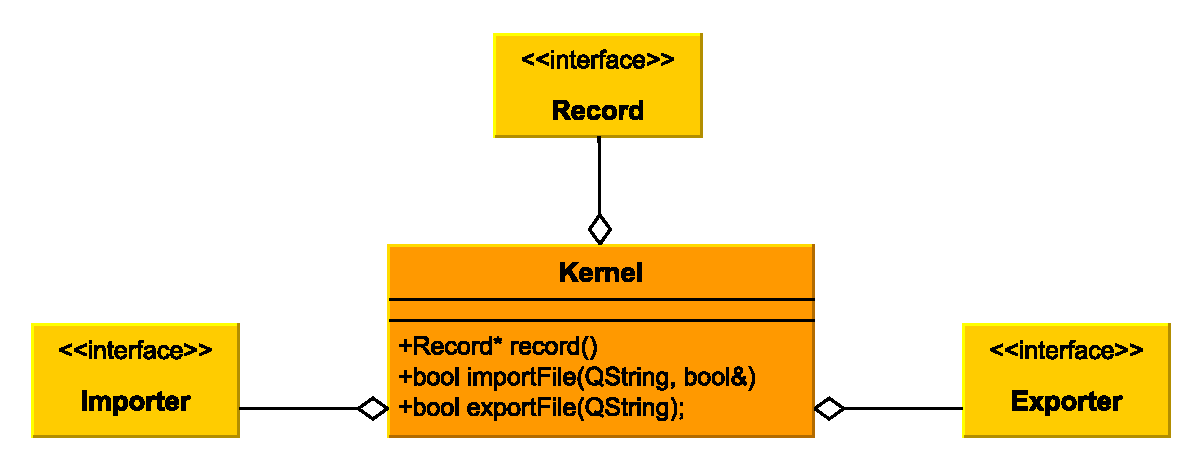
\includegraphics[width=13cm]{design/details/kernel/kernel.pdf}
			\caption{Třída \texttt{Kernel} a~její okolí}
			\label{fig:designDetailKernel}
		\end{figure}
		Třída \texttt{Kernel} zaštiťuje celé jádro aplikace. Obsahuje v~sobě ukazatele na rozhraní \texttt{Import}, \texttt{Export} a~\texttt{Record}, do nichž jsou instanciovány odvozené třídy s~vhodnou implementací, vybrané dle aktuálního použití aplikace. Rozhraní \texttt{Record} umožňuje přístup k~datům, rozhraní \texttt{Import} zprostředkovává načtení dat a~poslední rozhraní \texttt{Export} zajišťuje výstup evidovaných dat do souboru.\par
		Přestože tato třída zapouzdřuje veškeré datové operace aplikace, její návrh byl vytvořen tak, aby nebyla složitá ani její konstrukce, ani použití. Pro manipulaci s~daty slouží veřejná metoda \texttt{Record* record()}. Konkrétní přístup či modifikace už potom probíhají skrze ukazatel na rozhraní \texttt{Record}, který tato metoda poskytuje prostřednictvím své návratové hodnoty.\par
		Oproti tomu instance implementující rozhraní pro import a~export jsou před uživatelem třídy zcela skryty. Jejich funkcionalita je zprostředkována dvěma veřejnými metodami, z~nichž první slouží k~importování a~druhá k~exportování souboru. Formát souboru, a~tedy i~typ instanciované implementace rozhraní, je přitom determinován příponou parametrem předaného jména souboru. Pro vytvoření nového projektu s~prázdnými daty stačí volat importovací metodu s~prázdným parametrem jména souboru.\par
		Doporučené využití této třídy spočívá ve vytvoření jedné instance, která uživateli zprostředkuje funkcionality pro výměnu dat a~jejich správu. Vytvoření většího počtu instancí ale není zakázáno a~může být s~výhodou využito např. v~případě porovnávání dvou a~více rodokmenů.\par
		
		\subsection*{Rozhraní \texttt{Importer} a~\texttt{Exporter}}
		Funkcionality importu a~exportu dat jsou přístupné skrze rozhraní \texttt{Importer} a~\texttt{Exporter}. Rozhodnutí pro návrh těchto komponent za využití rozhraní plynulo z~flexibility, kterou rozhraní přinášejí. Díky nim je při rozšíření podpory importovacích a~exportovacích formátů možné tuto změnu rychle promítnout do aplikace prostřednictvím vytvoření nové implementace těchto rozhraní a~vhodným zakomponováním jejich instanciace do třídy \texttt{Kernel}. Zjednodušené diagramy, znázorňující návrh těchto dvou rozhraní, jsou k~nahlédnutí po řadě v~obrázku~\ref{fig:designDetailImporter} a~v~obrázku~\ref{fig:designDetailExporter}. \par
		\begin{figure}[H]
			\centering
			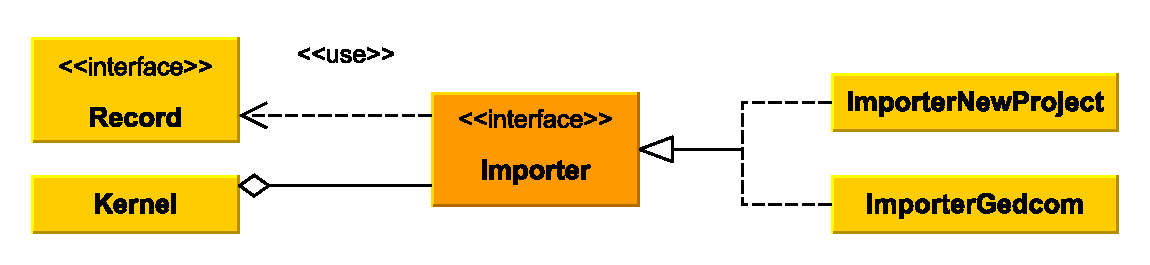
\includegraphics[width=12cm]{design/details/kernel/importer.pdf}
			\caption{Třída \texttt{Importer} a~její okolí}
			\label{fig:designDetailImporter}
		\end{figure}
		Rozhraní pro import a~export dat mají díky analogické funkcionalitě mnoho společných rysů, jsou tedy shrnuta v~této společné podsekci.  \par
		Obě tato rozhraní jsou velice jednoduchá. Typická je pro ně jediná veřejná metoda, jejíž implementace v~odvozených třídách se starají o~samotné předání dat. Obě tyto metody přijímají parametry v~podobě názvu souboru a~reference na implementaci rozhraní \texttt{Record}, které je využito buď jako cíl importu, nebo zdroj dat pro export. Metoda pro import má navíc parametr výčtového typu, který určuje, zda import probíhá ze souboru vytvořeného touto aplikací, nebo zda se jedná o~soubor z~jiné aplikace.\par
		\begin{figure}[H]
			\centering
			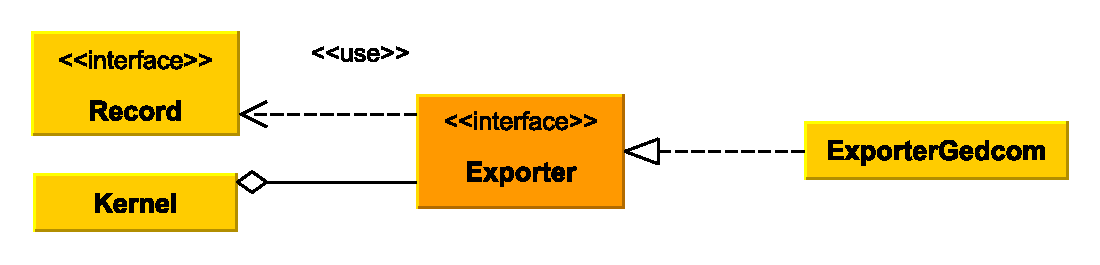
\includegraphics[width=12cm]{design/details/kernel/exporter.pdf}
			\caption{Třída \texttt{Exporter} a~její okolí}
			\label{fig:designDetailExporter}
		\end{figure}
		Rozhraní pro import je ještě obohaceno o~dvojici signálů. Tyto signály slouží k~vyrozumění uživatele tohoto rozhraní o~průběhu importu. První ze signálů je vyslán pouze jednou, a~to na začátku procesu importu. Tento signál podává informaci o~počtu struktur, které bude třeba importovat. Další signál je vyslán po každém úspěšném importování některé z~těchto struktur. Zpracováváním této kombinace signálů je možné počítat stav postupu importovacího procesu. \par
		
		\subsection*{Třídy \texttt{ImporterNewProject}, \texttt{ImporterGedcom} a~\texttt{ExporterGedcom}}
		Tato trojice tříd implementuje rozhraní \texttt{Importer} a~\texttt{Exporter} zmíněná v~předchozí podsekci. Prozatím jsou v~aplikaci dostupné dvě implementace importu a~jedna implementace exportu. Portfolio se může v~budoucnu rozšířit přidáním podpora souborových formátů. \par
		Třída \texttt{ImporterNewProject} provádí vytvoření nového genealogického projektu. Volání její importovací metody vede ke vzniku prázdné kolekce dat, kterou může uživatel dále libovolně modifikovat. \par
		I~třída \texttt{ImporterGedcom} stojí u~tvorby genealogického projektu, tentokrát ale probíhá import již existujících dat ze specifikovaného souboru ve formátu GEDCOM. Tento soubor je rozebrán a~podporovaná data jsou importována do programu. Tento proces byl zjednodušen použitím knihovny \emph{cgGedcom}~\cite{bib:LibCgGedcom} od Charlese Glancyho. Tato knihovna převádí značky ze souboru do vnitřní reprezentace, která je potom touto třídou převedena na samotná data. \par
		Oproti tomu třída \texttt{ExporterGedcom} se zabývá exportem dat z~jejich vnitřní reprezentace v~programu do souboru. Opět se jedná o~soubor ve formátu GEDCOM, což umožňuje sdílení dat vytvořených v~této aplikaci s~ostatními genealogickými programy. \par
		
		\subsection*{Rozhraní \texttt{Record}}
		Tato komponenta je nejklíčovější součástí jádra aplikace i~programu samotného. Stojí za tím skutečnost, že zprostředkovává jednotný přístup k~uloženým datům, přičemž způsob jejich uložení zůstává zapouzdřen. Skrze toto rozhraní je možné k~datům přistupovat, modifikovat je, odstraňovat, i~přidávat nové záznamy. Kromě zprostředkovávání těchto základních funkcionalit je rozhraní doplněno i~o~celou řadu dalších podpůrných metod. Zjednodušený diagram, znázorňující rozhraní a~jeho okolí, je k~nahlédnutí v~obrázku~\ref{fig:designDetailRecord}. \par
		\begin{figure}[H]
			\centering
			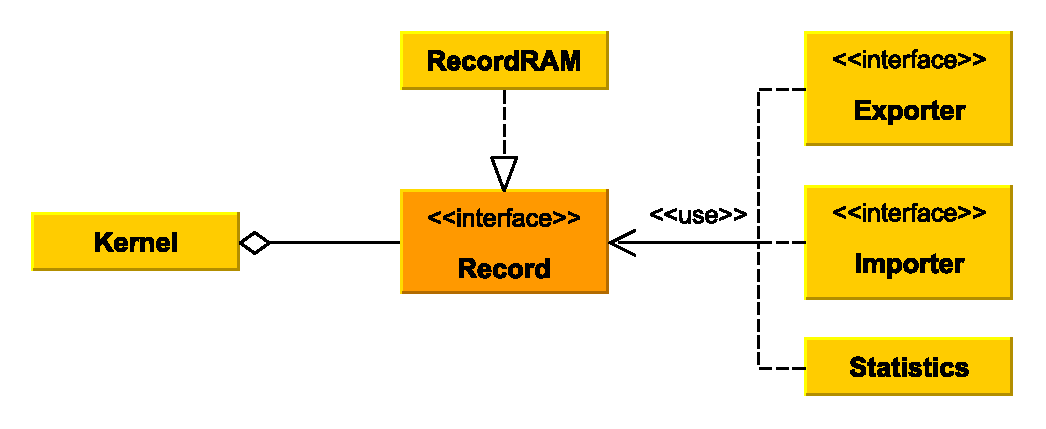
\includegraphics[width=12cm]{design/details/kernel/record.pdf}
			\caption{Třída \texttt{Record} a~její okolí}
			\label{fig:designDetailRecord}
		\end{figure}
		Veškerá komunikace s~rozhraním probíhá prostřednictvím předávání Identifikátorů typu \texttt{Identifier}. Tyto identifikátory jednoznačně určují každou zaznamenanou osobu, rodinu, zdroj i~přispěvatele. \par
		Rozhraní kompletně zapouzdřuje vnitřní reprezentaci dat v~implementaci. Vzhledem k~nutnosti pojmout široké spektrum funkcionality tedy není překvapením, že rozhraní obsahuje velký počet metod. Ty je možné pro lepší pochopení rozdělit do několika skupin. \par
		První skupina metod slouží k~vytváření nových záznamů. Tyto metody lze jednoduše rozpoznat dle předpony \texttt{new} v~názvu. Důležitým aspektem těchto metod je jejich návratová hodnota v~podobě identifikátoru, skrze nějž je možné vytvořenou entitu dále upravovat. \par
		Protipólem k~těmto metodám jsou metody odlišené předponou \texttt{delete} sloužící k~odstraňování záznamů. Zde je identifikátor naopak parametrem určujícím data k~odstranění. Za speciální zmínku stojí metoda \texttt{void deleteDatabase()}, která odstraní všechny záznamy. \par
		Další důležitou skupinou metod jsou validátory. Tyto metody jsou označené předponou \texttt{is} a~vrací booleovskou hodnotu. Jako parametr v~nich figuruje opět identifikátor. Jejich návratová hodnota odpovídá na otázku, kterou klade název metody samotné. Podává tedy např. informaci o~tom, zda byl dodaný identifikátor rozpoznán mezi záznamy jako identifikátor entity dotazovaného typu, nebo zda jsou či nejsou v~identifikovaném záznamu obsažena dotazovaná data. \par
		Nechybí ani skupina metod pro iteraci nad záznamy. Předpona těchto metod sestává z~výrazu \texttt{getIdentifier}, což je vodítko k~tomu, že návratová hodnota metod z~těchto skupiny je opět identifikátor. \par
		Následující skupina metod již slouží k~přístupu k~samotným datům, což naznačuje i~typická předpona \texttt{get}. Entita, jejíž data jsou žádána, je určena předaným identifikátorem. Metod tohoto typu rozhraní nabízí velký počet. Návratové hodnoty se liší dle dotazovaného typu dat. \par
		Kontrast tvoří další velká skupina sestávající z~metod pro úpravu dat. Jejich předpona je analogicky \texttt{set}, a~tentokrát je mezi parametry kromě identifikátoru předávána i~nová hodnota v~odpovídajícím datovém typu.\par
		Další malá skupina metod je uvozena předponou \texttt{swap}. Tyto metody slouží ke změně pořadí záznamů, což je užitečné například u~záznamů o~bydlišti či při řazení partnerů. \par
		Následuje skupina metod, která je do jisté míry podobná metodám na odstraňování dat. Metody z~této skupiny ale neodstraňují celé záznamy, nýbrž pouze odkazy v~podobě identifikátorů. Jejich předpona je tvořena slovem \texttt{remove}. \par
		Poslední skupinu tvoří sada nevirtuálních metod, které zajišťují doplňkové funkce. Tato skupina metod nelze specifikovat konkrétní předponou, jedná se ale převážně o~metody získávající seznamy všech použitých jmen či názvů míst a~o~několik dalších specifických metod.\par
		Toto rozhraní je aktuálně implementováno třídou \texttt{RecordRAM}. V~případě, že tato třída přestane být vyhovující, je možné ji v~budoucnu kdykoliv nahradit jinou komponentou či databází, a~to bez ohrožení funkcionality jakýchkoliv programů využívajících služeb jádra. \par
		Instanciace implementací tohoto rozhraní vně třídy \texttt{Kernel} není doporučena. Tato třída totiž zapouzdřuje i~funkcionality importu a~exportu. Ty by v~případě samostatného použití instance implementace tohoto rozhraní nebyly k~dispozici a~musely by být případně spravovány ručně uživatelem. \par
		
		\subsection*{Třída \texttt{RecordRAM}}
		Jak je znázorněno na obrázku~\ref{fig:designDetailRecordRAM}, tato třída implementuje rozhraní \texttt{Record}. Její hlavní zodpovědností je tedy evidence a~zpřístupnění genealogických dat prostřednictvím předepsaného rozhraní. K~naplnění tohoto cíle třída využívá celou řadu privátních atributů a~privátních metod.\par
		\begin{figure}[H]
			\centering
			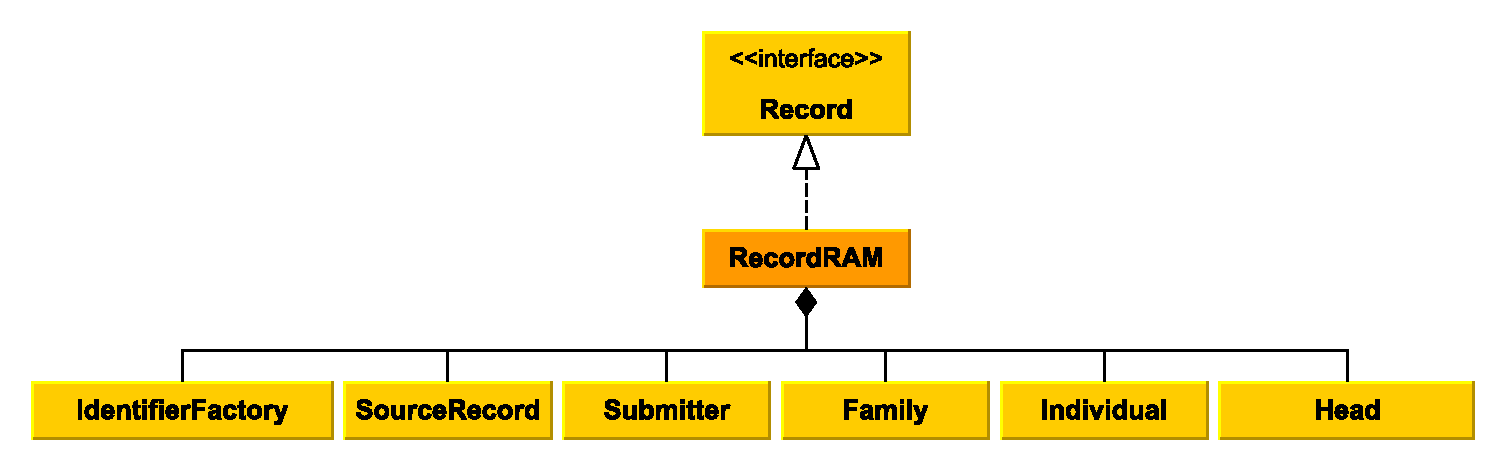
\includegraphics[width=15cm]{design/details/kernel/recordRam.pdf}
			\caption{Třída \texttt{RecordRAM} a~její okolí}
			\label{fig:designDetailRecordRAM}
		\end{figure}
		Struktura této třídy, a~především komponent v~ní uložených, byla inspirována způsobem správy dat definovaným ve standardu GEDCOM. Formátu odpovídá především způsob provázání uložených struktur v~podobě osob, rodin, zdrojů a~přispěvatelů s~rozšiřujícími strukturami, nesoucími např. informace o~narození, svatbě, či citacích. \par
		Třída v~sobě obsahuje celou řadu privátních atributů, zodpovědných za evidenci dat. Nejdůležitějšími z~nich jsou hašovací tabulky, které prostřednictvím klíče v~podobě identifikátoru poskytují přístup k~záznamům o~jednotlivých osobách \texttt{Individual}, rodinách \texttt{Family}, přispěvatelích \texttt{Submitter} a~zdrojích \texttt{SourceRecord}. Nechybí ani struktura evidující obecné informace o~genealogickém projektu. \par
		Dále jsou zde uloženy instance továren třídy \texttt{IdentifierFactory}, které produkují validní jedinečné identifikátory pro označení nově přidaných struktur. \par
		Návrh třídy klade důraz na to, aby byla v~plné míře naplněna specifikace metod rozhraní. Jedním z~klíčových a~všeobecných požadavků na tyto metody je požadavek na jejich stabilitu. Při volání metod nesmí dojít k~selhání a~za všech okolností musí být navrácena validní hodnota. V~případě, že byl proveden dotaz na neexistující strukturu, je za validní chování považováno navrácení prázdné hodnoty či jejího ekvivalentu. \par
		Tato skutečnost vede k~vysoké míře stability datového úložiště jádra aplikace. Jelikož dotazy na data jsou nejčastějším případem užití jádra, celistvá implementace, odolná proti selhání, tvoří pevný a~spolehlivý základ pro jakoukoliv přidanou nadstavbu.\par
		
		\subsection*{Třída \texttt{Identifier} a~podpůrné třídy}
		Instance třídy \texttt{Identifier} slouží primárně k~jednoznačné identifikaci dat. Jsou jejich prostřednictvím identifikovány jednotlivé osoby, rodiny, zdroje i~přispěvatelé. Třída je společně s~okolím znázorněna na obrázku~\ref{fig:designDetailIdentifier}.\par
		\begin{figure}[h]
			\centering
			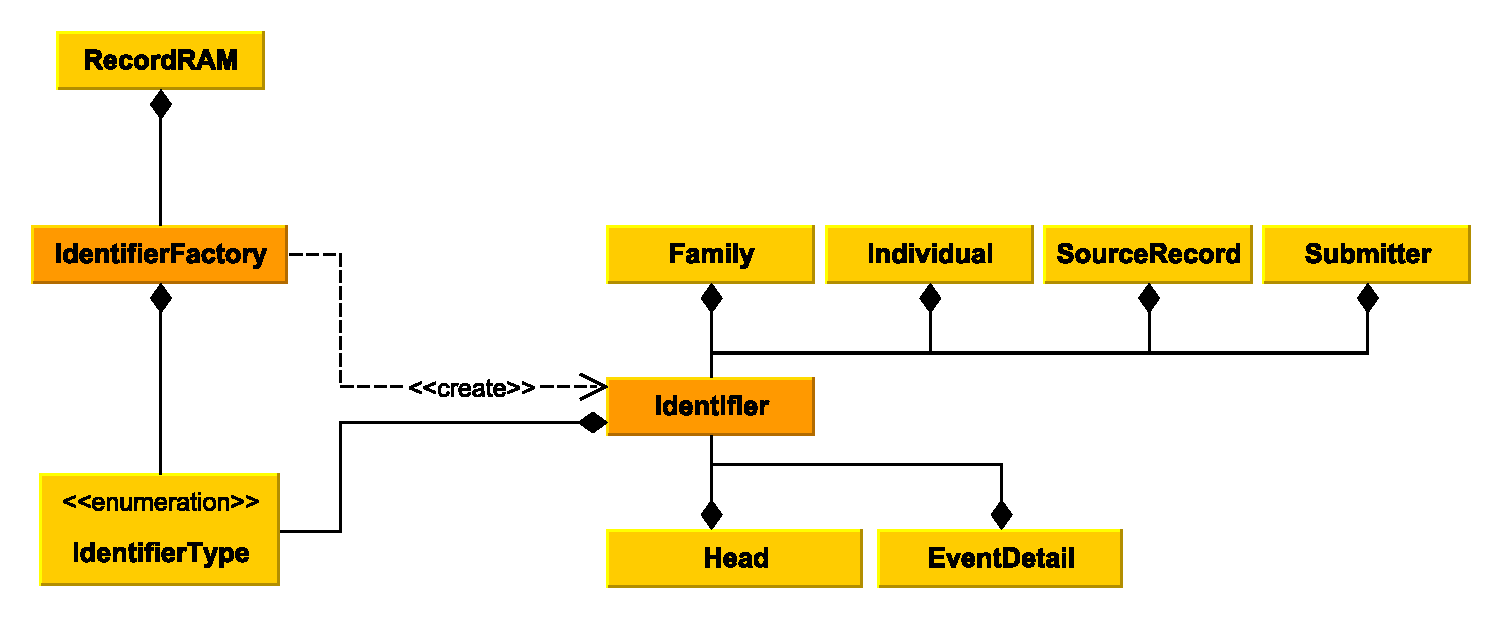
\includegraphics[width=15cm]{design/details/kernel/identifier.pdf}
			\caption{Třída \texttt{Identifier} a~její okolí}
			\label{fig:designDetailIdentifier}
		\end{figure}
		Schopnost instancí této třídy jednoznačně určit konkrétní data je jádrem aplikace široce využívána. Slouží díky tomu také jako komunikační prostředek mezi implementací rozhraní \texttt{Record} a~jeho uživatelem. Veškerá komunikace s~rozhraním pro přístup k~datům totiž probíhá prostřednictvím předávání instancí identifikátorů. Volaná metoda potom na základě identifikátoru provede vybranou operaci s~daty identifikované entity. \par
		Další zodpovědností instancí této třídy je tvoření vazeb mezi daty. Identifikátory jsou použity např. k~reprezentaci partnerů a~potomků v~záznamech o~rodině, nebo při identifikaci citovaného zdroje u~události. \par
		Třída je navržena tak, že volání veřejného konstruktoru vede k~vytvoření instance identifikátoru, který je neplatný. Aby byl identifikátor validní, musí být zkonstruován skrze továrnu \texttt{IdentifierFactory}. \par
		Jak již název třídy \texttt{IdentifierFactory} napovídá, jedná se o~továrnu na instance identifikátorů. Při její konstrukci byl využit návrhový vzor továrna. \par
		Instancím této tovární třídy je při inicializaci předána hodnota výčtového typu, která determinuje typ entity, pro niž má továrna identifikátory produkovat. Pro vygenerování identifikátoru potom stačí provést volání metody \texttt{Identifier newIdentifier()}. Ta má přístup ke chráněnému konstruktoru třídy \texttt{Identifier}, s~jehož pomocí zkonstruuje platný identifikátor odpovídajícího typu a~předá ho volajícímu prostřednictvím návratové hodnoty.\par
		
		\subsection*{Třída \texttt{Individual} a~podpůrné třídy}
		Třída \texttt{Individual} ukládá data náležící konkrétní evidované osobě, jak je znázorněno v~obrázku~\ref{fig:designDetailIndividual}. Chráněný konstruktor zajišťuje, že její instance mohou být tvořeny pouze v~rámci instancí spřátelené třídy \texttt{RecordRAM}. \par
		\begin{figure}[h]
			\centering
			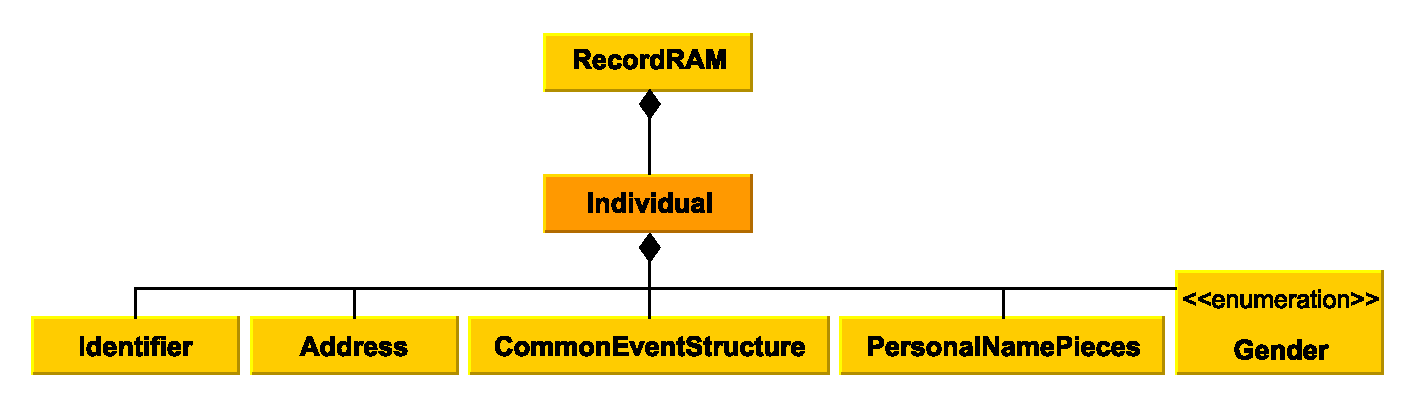
\includegraphics[width=14cm]{design/details/kernel/individual.pdf}
			\caption{Třída \texttt{Individual} a~její okolí}
			\label{fig:designDetailIndividual}
		\end{figure}
		Struktura třídy byla odvozena od stavby záznamu o~osobě dle standardu GEDCOM. Je v~ní evidován vlastní identifikátor osoby, struktura pro uložení jmen osoby a~atribut výčtového typu zachycující pohlaví osoby. Nechybí ani hašovací tabulka se záznamy o~událostech týkajících se dané osoby a~vektory struktur pro zaznamenání bydliště, zaměstnání, vzdělání a~náboženského vyznání osoby. Obsažen je i~atribut pro zaznamenání vlastních poznámek k~osobě. \par
		Za zvláštní zmínku stojí třída \texttt{PersonalNamePieces} evidující jména dané osoby. Její struktura umožňuje uložit jméno, příjmení za svobodna, vyvdané příjmení a~tituly před a~za jménem. Přístup a~úprava atributů je prováděna pomocí běžných get a~set metod. \par
		Výčtový typ \texttt{Gender}, který zachycuje pohlaví osoby, umožňuje evidencí tří typů hodnot. Hodnoty pro muže a~ženu, které jsou samozřejmostí, jsou doplněny hodnotou vyjadřující skutečnost, že pohlaví osoby není známé. \par
		U~osob je možné evidovat záznamy o~událostech typu narození, křest, úmrtí a~pohřeb. Je zřejmé, že každý z~těchto záznamů se u~osoby může vyskytovat maximálně jedenkrát.\par
		Naopak struktury evidující bydliště, zaměstnání, vzdělání a~náboženské vyznání mohou obsahovat libovolný počet záznamů. Pořadí záznamů v~těchto jednotlivých kategoriích je uživatelsky upravitelné.\par
				
		\subsection*{Třída \texttt{Family}}
		Třída \texttt{Family} slouží k~uložení dat o~rodině. Společně se svým okolím je třída znázorněna v~obrázku~\ref{fig:designDetailFamily}. Instance třídy jsou tvořeny chráněným konstruktorem, který je dostupný pouze instancím spřátelené třídy \texttt{RecordRAM}.\par
		\begin{figure}[h]
			\centering
			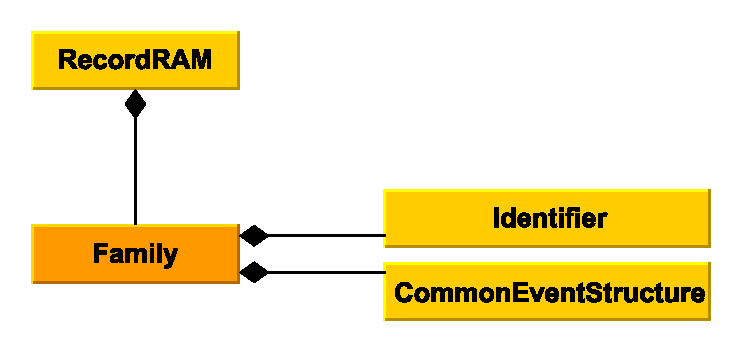
\includegraphics[width=8cm]{design/details/kernel/family.pdf}
			\caption{Třída \texttt{Family} a~její okolí}
			\label{fig:designDetailFamily}
		\end{figure}
		Obsah třídy je vytvořen jako analogie záznamu o~rodině definovaného standardem GEDCOM. Hlavní zodpovědností této struktury je definovat mezi jednotlivými osobami rodinné vztahy a~propojovat je tak do stromu příbuzenství.\par
		Rodina je zde definována jako partner, partnerka a~jejich společné děti. Platí přitom, že ne všechny tyto role musí být využity. Validní je tedy i~například rodina tvořená bezdětnými partnery nebo pouze partnerkou a~jejími dětmi. \par
		Každá rodina má vlastní jednoznačný identifikátor. Dále obsahuje identifikátory osob v~ní figurujících, tedy identifikátor partnera, identifikátor partnerky a~vektor identifikátoru jejich potomků. Nepřítomnost osoby zastávající některou z~těchto rolí je reprezentována buď neplatným identifikátorem u~chybějícího partnera či partnerky, nebo prázdným vektorem pro zaznamenávání potomků.\par
		U~rodiny je dále možné zaznamenat události. Jedná se o~sňatek a~rozvod figurujících partnerů. Každá z~těchto událostí může být pro zjednodušení zaznamenána pouze jedenkrát. \par
		
		\subsection*{Třída \texttt{SourceRecord} a~podpůrné třídy} % zdroje + citace
		Tato třída zaznamenává data o~evidovaných zdrojích. Zdrojem je v~tomto kontextu myšlena matrika obsahující záznamy o~narození, sezdání či úmrtí osob. Třída a~její vazby na okolí jsou znázorněny v~obrázku~\ref{fig:designDetailSourceRecord}. Chráněný konstruktor zamezuje tvoření instancí třídy \texttt{SourceRecord} mimo instance spřátelené třídy \texttt{RecordRAM}.\par
		\begin{figure}[h]
			\centering
			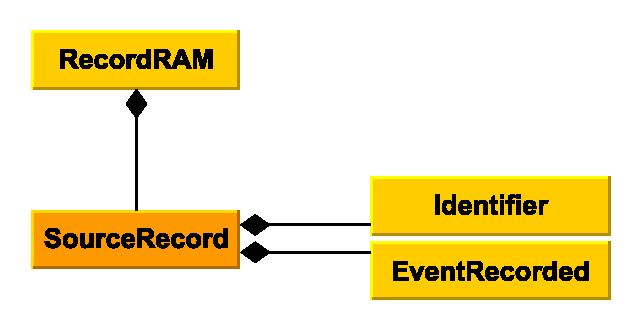
\includegraphics[width=7cm]{design/details/kernel/sourceRecord.pdf}
			\caption{Třída \texttt{SourceRecord} a~její okolí}
			\label{fig:designDetailSourceRecord}
		\end{figure}
		Struktura třídy vychází ze složení záznamu o~zdroji dle standardu GEDCOM. Každá instance je označena jedinečným identifikátorem. Mezi evidovaná data patří název archivu, signatura matriky a~její původce. Je možné evidovat i~odkaz na web, z~něhož je dostupná digitalizovaná kopie materiálu.\par
		Dále je možné uložit záznamy o~evidovaných událostech. Podporována je evidence událostí typu narození, sňatek a~úmrtí. Záznamy o~přítomnosti těchto událostí jsou evidovány prostřednictvím instancí třídy \texttt{EventRecorded}. V~těchto instancích jsou uchovávána data o~místě, časovém rozpětí zdroje, rozsahu stran, zabývajících se touto oblastí a~nechybí ani možnost zaznamenání odkazu na počáteční stranu příslušné digitalizované matriky.\par
		
		\subsection*{Třída \texttt{Submitter}}
		Třída \texttt{Submitter} je nejjednodušší ze čtveřice základních tříd. Společně se svým okolím je k~nahlédnutí v~obrázku~\ref{fig:designDetailSubmitter}. Eviduje data o~přispěvateli. Tvoření instancí je regulováno chráněným konstruktorem, který je přístupný pouze spřátelené třídě \texttt{RecordRAM}.\par
		\begin{figure}[h]
			\centering
			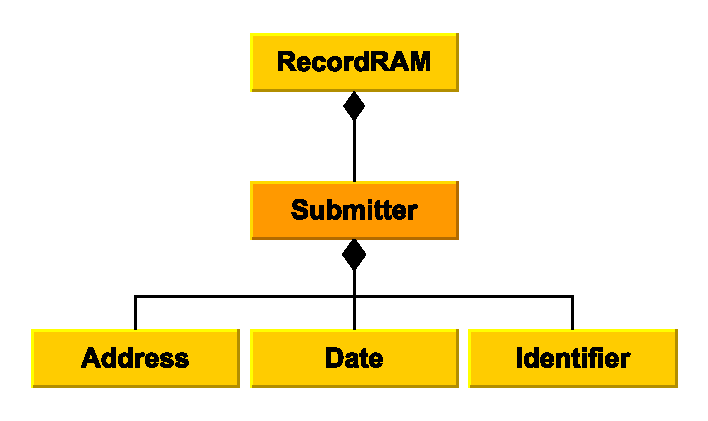
\includegraphics[width=8cm]{design/details/kernel/submitter.pdf}
			\caption{Třída \texttt{Submitter} a~její okolí}
			\label{fig:designDetailSubmitter}
		\end{figure}
		Inspirací pro strukturu této třídy bylo složení záznamu o~přispěvateli definovaného ve standardu GEDCOM. Každému přispěvateli je při konstrukci přiřazen jednoznačný identifikátor. Dále je možné v~něm evidovat data o~jméně, adrese, preferovaném jazyce a~doplnit záznam poznámkami. Ukládá se i~datum a~čas poslední modifikace souboru, která byla přispěvatelem provedena.\par
		
		\subsection*{Třída \texttt{CommonEventStructure} a~podpůrné třídy}
		Tato třída slouží k~zaznamenávání událostí a~jejich podrobností. Náhled jejího okolí je k~dispozici v~obrázku~\ref{fig:designDetailCommonEventStructure}. Pojem událost v~tomto kontextu zahrnuje narození, křest, úmrtí, pohřeb, sňatek, rozvod, změnu bydliště, dovršení vzdělání, pracovní zkušenost a~příslušnost k~náboženské skupině. Jedná se o~výběr událostí a~atributů převzatých ze standardu GEDCOM. \par
		Typ události je dán při konstrukci hodnotou výčtového typu. Dále je možné evidovat slovní popis události. K~uložení podrobností slouží instance třídy \texttt{EventDetail}.\par
		\begin{figure}[h]
			\centering
			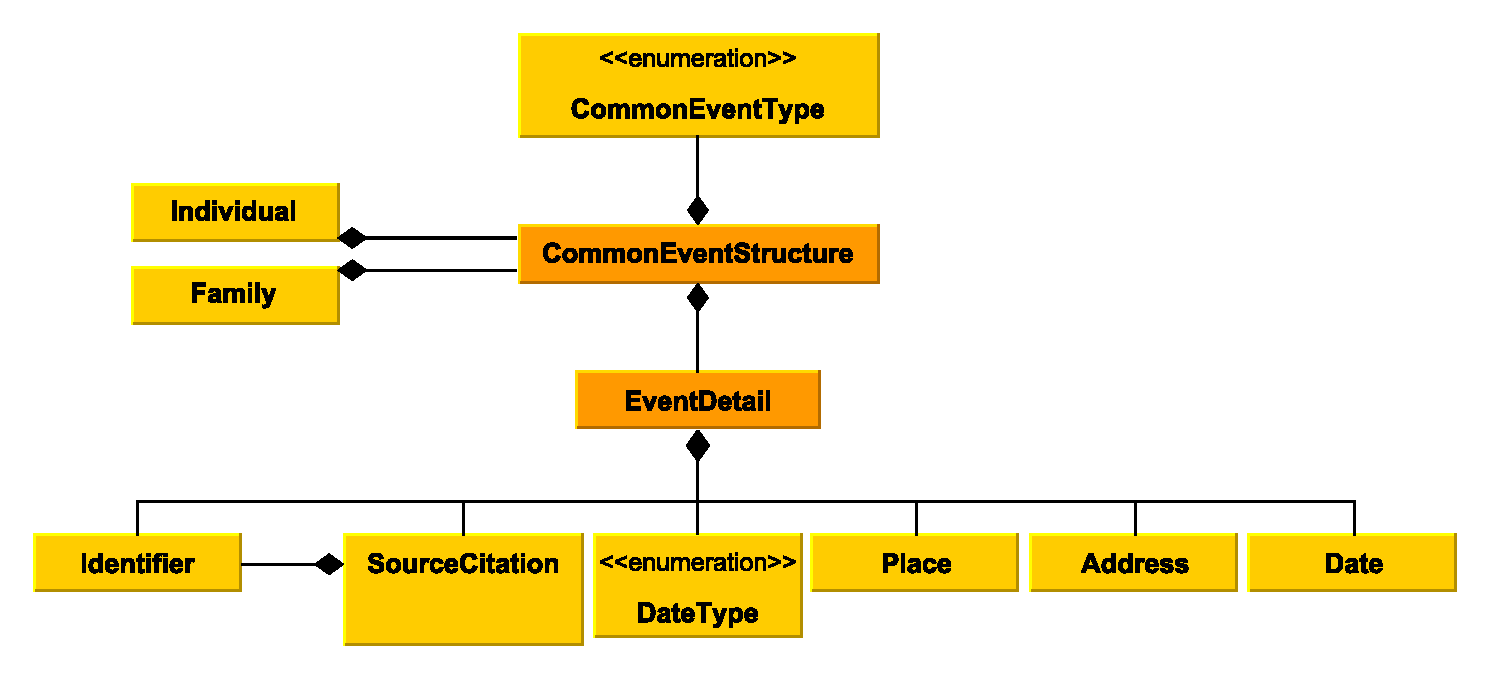
\includegraphics[width=15cm]{design/details/kernel/commonEventStructure.pdf}
			\caption{Třída \texttt{CommonEventStructure} a~její okolí}
			\label{fig:designDetailCommonEventStructure}
		\end{figure}
		Podrobnosti události obsahují slovní klasifikaci události, údaje o~datu či časovém rozpětí, data o~místě, adrese a~příčině. \par
		Dle navrhované aktualizace specifikace formátu GEDCOM jsou zde obsaženy i~identifikátory odkazující na osoby, které s~událostí souvisí. Tyto osoby jsou označeny jako kněz, svědek č.~1 a~svědek č.~2. Bližší popis jejich rolí je zaznamenán v~sekci~\ref{sec:designGedcom}.\par
		Za speciální zmínku stojí také údaj o~citovaném zdroji. Ten je evidován v~instanci třídy \texttt{SourceCitation}. Identifikátor, odkazující na citovaný zdroj, je zde doplněn daty o~straně, kde se citovaný zápis nachází. Je také možné doplnit odkaz na příslušnou stranu digitalizované matriky. \par
		
		\subsection*{Třída \texttt{Statistics}}
		Třída \texttt{Statistics} slouží k~vytváření statistik nad daty, která jsou přístupná skrze rozhraní \texttt{Record}. V~současné fázi návrhu se jedná především o~reprezentaci možného směru dalšího vývoje aplikace. Vazby této třídy na okolí jsou k~nahlédnutí v~obrázku~\ref{fig:designDetailStatistics}. \par
		\begin{figure}[h]
			\centering
			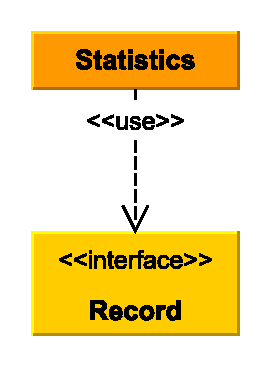
\includegraphics[width=3cm]{design/details/kernel/statistics.pdf}
			\caption{Třída \texttt{Statistics} a~její okolí}
			\label{fig:designDetailStatistics}
		\end{figure}
		Současná reprezentace třídy obsahuje privátní referenci na rozhraní záznamů. Výběr veřejných metod aktuálně zahrnuje metodu pro získání základních metrik rodokmenu. Mezi ně patří údaje o~počtu generací, celkovém počtu osob, počtu osob dle pohlaví a~počtu žijících osob. Navržena je i~metoda pro získání údaje o~osobě s~nejnižším a~nejvyšším dožitým věkem. \par
		Tato třída by mohla být v~budoucnu rozšířena o~celou řadu dalších statistických funkcí. Ty jsou prospěšné nejen z~pohledu, že uživateli zprostředkovávají obecný přehled nad evidovanými daty, ale mohou často vést i~k~odhalení chybně zadaných dat. \par
		
		\subsection*{Třída \texttt{Date}}
		Tato třída je odvozena od bázové třídy \texttt{QDate} převzaté z~frameworku Qt. Tato bázová třída slouží pro správu kalendářních dat. Neumožňuje však ukládání nepřesných dat, která sestávají pouze z~roku či roku a~měsíce. \par
		Jelikož je nutné, aby jádro takovouto funkcionalitu nabízelo, došlo k~vytvoření třídy \texttt{Date}. Třída v~sobě eviduje hodnotu enumerace \texttt{DatePrecision}. Ta zaznamenává přesnost data ve čtyřech úrovních~--~zcela přesné datum, přesný měsíc a~rok, přesný pouze rok a~prázdné datum. Třída \texttt{Date} a~její vazby na okolí jsou k~nahlédnutí v~obrázku~\ref{fig:designDetailDate}.\par
		\begin{figure}[h]
			\centering
			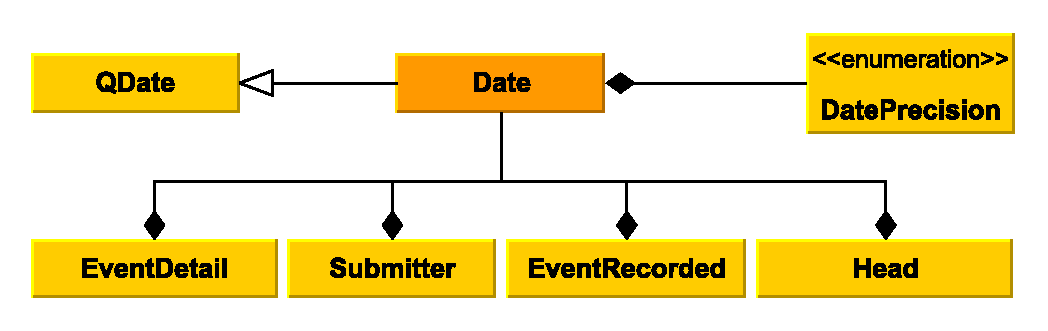
\includegraphics[width=12cm]{design/details/kernel/date.pdf}
			\caption{Třída \texttt{Date} a~její okolí}
			\label{fig:designDetailDate}
		\end{figure}
	
	\newpage
	% Návrh uživatelského rozhraní aplikace
	
	\section{Návrh uživatelského rozhraní aplikace}
	Dobře navržené uživatelské rozhraní vždy patří mezi důležité faktory determinující úspěch aplikace jako celku. Návrh uživatelského rozhraní je tedy velice důležitou součástí celého procesu návrhu. \par
	Jelikož vývoj uživatelského rozhraní aplikace následoval spirálový model, bude zde popsána až konečná verze návrhu uživatelského rozhraní.\par
	Za samotnou myšlenkou nové genealogické aplikace stál záměr vytvořit program s~jednoduchým a~rychle ovladatelným uživatelským rozhraním, který mimo jiné umožní editaci všech zásadních informací o~osobě v~jediném okně. Je tedy zřejmé, že návrh uživatelského rozhraní aplikace byl jedním z~klíčových kroků, determinujících úspěch celého programu a~naplnění jeho specifikace.\par
	Jelikož je rozhraní aplikace tvořeno 135 třídami, nebude jeho diagram jako celku zahrnut. Uživatelské rozhraní je ale přehledně zpracováno v~dokumentaci na přiloženém médiu. Cesta k~dokumentaci je popsána v~příloze~\ref{append:cd}. 
	Program byl pojmenován \emph{ProGenealogy}. Jelikož je aplikace cílena primárně na české uživatele, je i~její název převzat primárně z~češtiny a~vyjadřuje, že se jedná o~aplikaci vytvořenou \uv{pro genealogy}. Ani cizojazyční uživatelé ovšem nepřijdou zkrátka, jelikož předpona \emph{Pro} je v~názvech programů často používána a~může být chápána jako zkrácená verze anglického slova \uv{professional}. Druhá část názvu, \emph{Genealogy}, je potom internacionalismus označující rodopis jako pomocnou vědu historickou.\par
	Přestože aplikace funguje nativně v~angličtině, uživatelské rozhraní je navrženo tak, aby bylo možné lokalizovat jej i~do češtiny a~dalších jazyků. Bude tak splněna nutná podmínka pro rozšíření aplikace do komunity českých a~slovenských genealogů, a~dveře zůstanou otevřené i~možnosti případné expanze do zahraničí.\par
	Aplikace jako celek je spouštěna skrze funkci \texttt{int main()}. V~těle této funkce je vytvořena instance třídy jádra \texttt{Kernel}. Reference na tuto instanci je předána konstruktoru třídy hlavního okna aplikace. Instance hlavního okna aplikace je poté zobrazena uživateli a~je spuštěna hlavní aplikační smyčka.\par
	
	% Připsat sekci o tom, jak by se mělo navrhovat UI - zdůvodnit obrázkové ikony doplněné o tooltipy
		
		\subsection*{Třída \texttt{MainWindow}}
		Uživatelské rozhraní jako celek je zaštítěno třídou \texttt{MainWindow}. Tato třída má celou řadu pravomocí, ovlivňujících chod celé aplikace. Především ale působí jako kontejner pro všechny prvky základního grafického uživatelského rozhraní, jak je znázorněno v~obrázku~\ref{fig:designDetailMainWindow}.\par
		\begin{figure}[h]
			\centering
			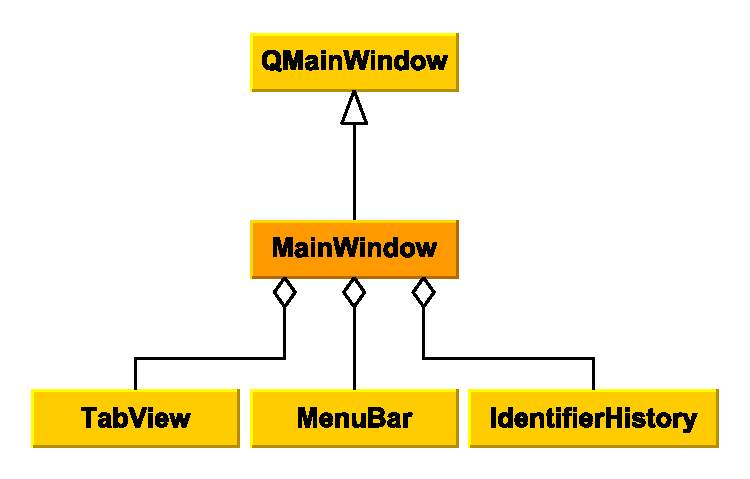
\includegraphics[width=9cm]{design/details/ui/mainWindow.pdf}
			\caption{Třída \texttt{MainWindow} a~její okolí}
			\label{fig:designDetailMainWindow}
		\end{figure}
		Třída v~sobě uchovává referenci na instanci jádra, která zprostředkovává celému uživatelskému rozhraní přístup k~datům. Kromě toho udržuje hodnoty dvou důležitých identifikátorů. Jedná se o~identifikátor osoby, která je uživatelem aktuálně spravována, tzv. probanda, a~o~identifikátor aktuálně vybraného zdroje. \par
		Jakákoliv změna těchto hodnot je do této třídy propagována za použití signálu \texttt{void probandChanged(const Identifier ref)}. Ten zde vyvolá členskou metodu, která se postará o~provedení všech nutných změn a~o~aktualizaci všech prvků rozhraní, které jsou změnou ovlivněny. \par
		Konkrétně s~identifikátorem, určujícím probanda, souvisí další třída, jejíž instance je ve třídě \texttt{MainWindow} uchovávána. Jedná se o~instanci třídy \texttt{IdentifierHistory}, která pro potřeby uživatele uchovává nastavitelný počet historicky vybraných probandů. \par
		Třída také spravuje instance, které se starají o~zobrazení textů grafického rozhraní ve správném jazyce. Spravovány jsou dvě instance, přičemž jedna je zodpovědná za překlad textových řetězců specifických pro aplikaci, druhá potom za řetězce předdefinované použitým frameworkem.\par
		Prozatím zdokumentované náležitosti třídy patří mezi ty, které pro uživatele nejsou viditelné. Třída ovšem spravuje všechny komponenty základního grafického uživatelského rozhraní. Děje se tak díky instancím dvěma tříd.\par 
		První z~nich je třída \texttt{MenuBar}, která spravuje nabídku menu aplikace a~akce, které jsou výběrem jednotlivých položek menu vyvolány. Další je potom třída \texttt{TabView} zobrazující samotný obsah okna.\par
		
		\subsection*{Třída \texttt{IdentifierHistory}}
		Tato třída slouží ke správě historicky vybraných identifikátorů. Může se jednat jak o~identifikátory osob, tak i~o~identifikátory jakýchkoliv dalších struktur, např. zdrojů. V~současné době je ale tato třída využita pouze pro zaznamenávání historického výběru osob. Třída je se svým okolím znázorněna v~obrázku~\ref{fig:designDetailIdentifierHistory}.\par
		\begin{figure}[h]
			\centering
			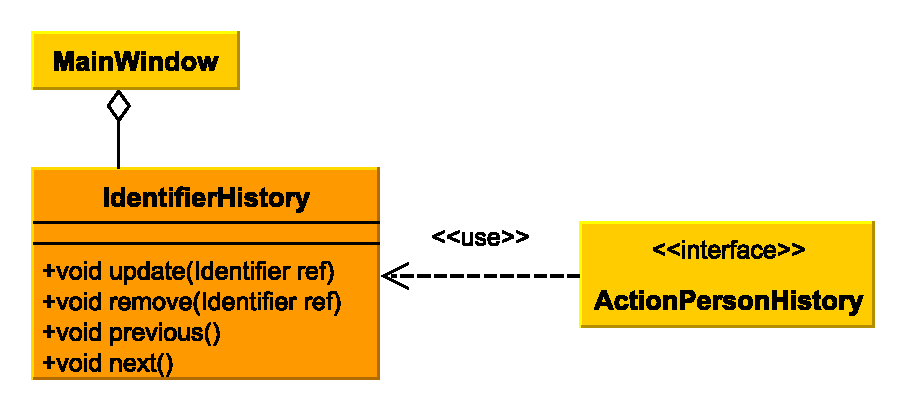
\includegraphics[width=11cm]{design/details/ui/identifierHistory.pdf}
			\caption{Třída \texttt{IdentifierHistory} a~její okolí}
			\label{fig:designDetailIdentifierHistory}
		\end{figure}
		Při instanciaci třídy je nutné dodat konstruktoru parametr, který stanovuje maximální počet identifikátorů evidovaných v~historii. Tímto krokem se zamezí situaci, kdy by se hloubka historie s~každou další vybranou osobou rozrůstala a~evidence historie by tak zabírala čím dál více paměti. Pokud je tato kapacita překročena, dojde k~odstranění nejstarších položek historie.\par
		Rozhraní třídy nabízí metodu \texttt{void update(Identifier ref)}, která přidá do paměti historie parametrem předaný identifikátor. Dále jsou k~dispozici metody \texttt{void previous()} a~\texttt{void next()}, které provádějí samotný posun v~historii. Ten je proveden zasláním příslušného signálu třídě \texttt{MainWindow}. V~případě, že posun na předchozí či následující osobu není možný (např. v~případě prázdné historie), jsou tyto metody bez efektu.\par
		Pokud v~programu dojde k~odstranění entity, která je v~historii evidována, je nutné ji z~historie vymazat použitím metody \texttt{void remove(Identifier ref)}. Celou historii je potom možné vrátit do výchozího stavu voláním metody \texttt{void reset()}.\par
		
		\subsection*{Třída \texttt{MenuBar}}
		Tato třída eviduje všechna menu a~akce obsažená v~hlavní nabídce programu. Skrze vyvolání těchto akcí jsou zprostředkovány dialogy pro import či export dat, akce pro práci s~daty v~programu případně dialogy pro úpravu nastavení aplikace. Diagram znázorňující strukturu menu a~v~něm obsažených akcí je k~nahlédnutí v~obrázku~\ref{fig:designDetailMenuBar}.\par
		\begin{figure}[t!]
			\centering
			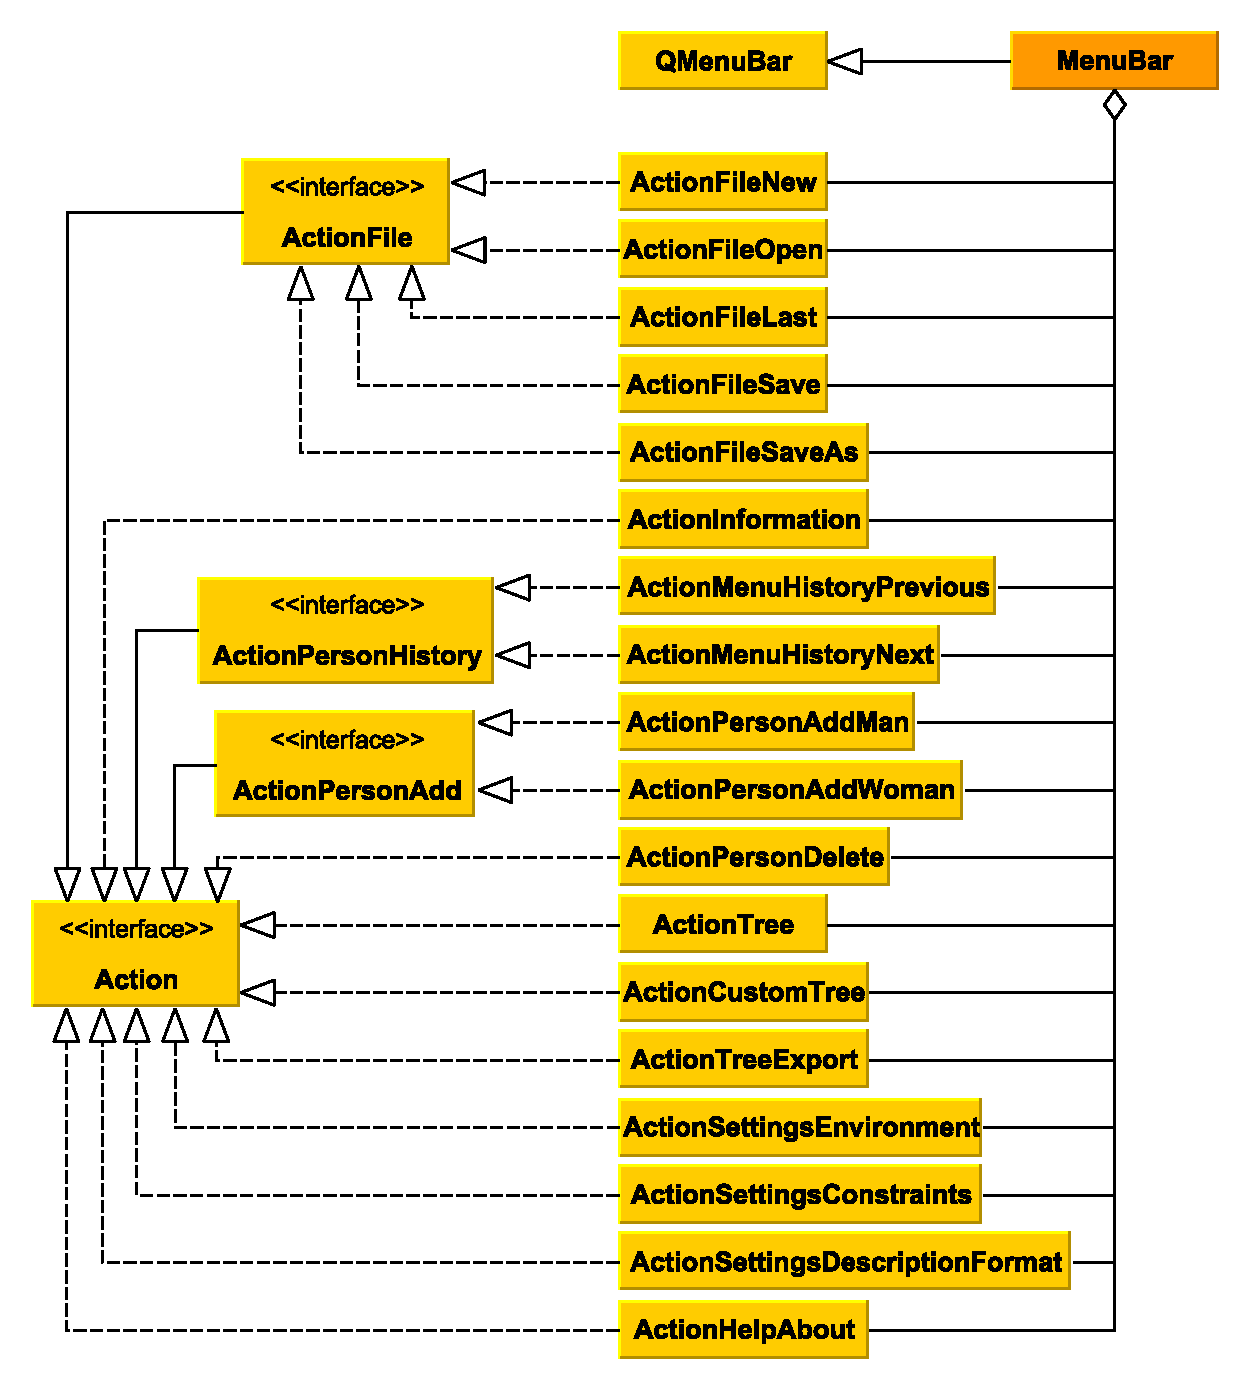
\includegraphics[width=13.5cm]{design/details/ui/menuBar.pdf}
			\caption{Třída \texttt{MenuBar} a~její okolí}
			\label{fig:designDetailMenuBar}
		\end{figure}
		První z~nabídek je nabídka související s~aktuálním souborem. Zde je možné vytvořit nový genealogický projekt, otevřít či importovat existující projekt ve formátu GEDCOM, uložit aktuální data, nebo upravit informace o~rodokmenu jako celku. K~dispozici je i~rychlý výběr z~až pěti souborů, které byly v~nedávné době importovány. Všechny nabízené akce jsou zaštítěny třídami implementujícími rozhraní \texttt{ActionFile}, vyjma akce na editaci informací o~rodokmenu \texttt{ActionInformation}. \par
		Další položka nabídky se týká osoby. Skrze tuto nabídku je možné používat akce pro pohyb v~historii vybraných osob. Třídy poskytující tyto akce implementují rozhraní, které je definované třídou \texttt{ActionPersonHistory}. Také je možné vytvářet nové záznamy o~osobách, a~to skrze instance tříd implementující rozhraní \texttt{ActionPersonAdd} a~odstraňovat existující záznamy prostřednictvím vyvolání akce \texttt{ActionPersonDelete}. \par
		V~menu je k~dispozici také nabídka spravující vykreslování stromů. Skrze akce z~této nabídky je možné vykreslovat stromové diagramy. Tyto akce jsou zapouzdřeny třídou \\ \texttt{ActionTree}. Aktuálně je k~dispozici tvorba vývodu z~předků, agnátního a~kognátního vývodu, rozrodu rodu a~stromu příbuzenstva. Poslední položka v~této nabídce, zaštítěna třídou \texttt{ActionTreeExport} umožňuje provedení exportu vygenerovaného diagramu do rastrových obrázků nebo do formátu pdf. Uživatelé tak mohou s~vygenerovanými diagramy dále pracovat i~mimo aplikaci.\par
		Další nabídka umožňuje úpravu chování programu prostřednictvím nastavení. Uživateli jsou přístupná nastavení jazyka, automatického otevření posledního načteného souboru, a~také nastavení formátu textových výpisů programu.\par
		Poslední položka nabídky menu využívá akci \texttt{ActionHelpAbout} a~slouží ke zobrazení informací o~aplikaci. Jsou zde vypsány informace o~aktuální verzi programu, použité verzi frameworku Qt, a~licenci. \par
		Nejčastěji používaným akcím z~nabídky menu byly přiřazeny i~klávesové zkratky. Tato skutečnost zrychlí a~zpříjemní pokročilým uživatelům interakci s~programem. Univerzálně používané klávesové zkratky jsou navíc poplatné platformě, na níž je program spouštěn. Uživatelé Linuxových systémů tak nebudou nuceni si zvykat na klávesové zkratky typické pro systémy Windows, a~podobně. \par
		
		\subsection*{Třída \texttt{TabView}}
		Třída \texttt{TabView} je vstupním portálem do základního rozhraní aplikace. Reprezentuje zobrazení se záložkami, které zaplňuje celé hlavní okno aplikace, a~obsahuje v~sobě entity definující jednotlivé záložky, jak je znázorněno v~obrázku~\ref{fig:designDetailTabView}. \par
		\begin{figure}[h]
			\centering
			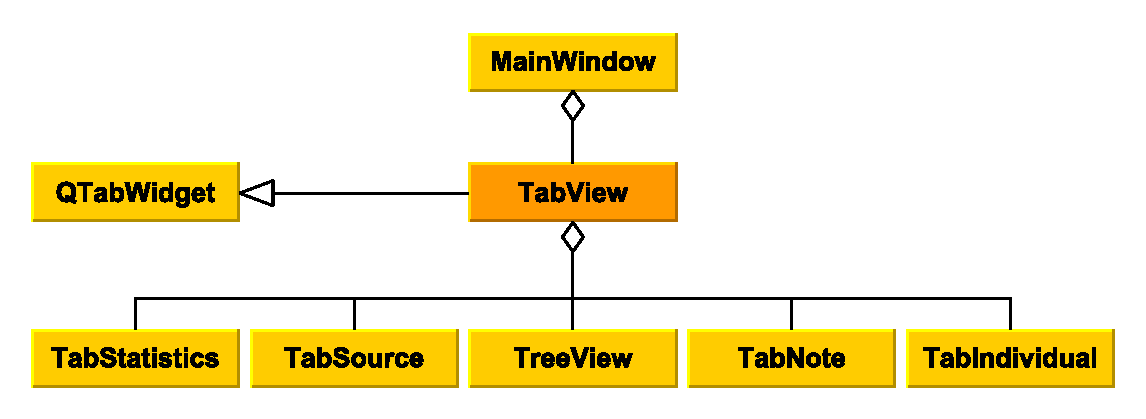
\includegraphics[width=13cm]{design/details/ui/tabView.pdf}
			\caption{Třída \texttt{TabView} a~její okolí}
			\label{fig:designDetailTabView}
		\end{figure}
		Jedná se o~strukturu, která spravuje jednotlivé prvky rozhraní a~zprostředkovává jejich komunikaci se správcovskou třídou \texttt{MainWindow}. Tato třída také umožňuje automatické změny aktuální záložky, např. v~případě, kdy je vykreslen strom, je pozornost automaticky přesunuta na záložku, kde je vygenerované zobrazení k~nahlédnutí. \par
		
		\subsection*{Třída \texttt{TabIndividual}}
		Tato třída implementuje grafické rozložení rozhraní na záložce osoby. Zapouzdřuje komponenty uživatelského rozhraní pro zobrazování a~editaci dat o~jednotlivých osobách. Titulek záložky je tvořen uživatelsky přívětivým řetězcem, který identifikuje aktuálně zobrazovanou osobu. Struktura okolí třídy je k~nahlédnutí v~obrázku~\ref{fig:designDetailTabIndividual}.\par
		\begin{figure}[h]
			\centering
			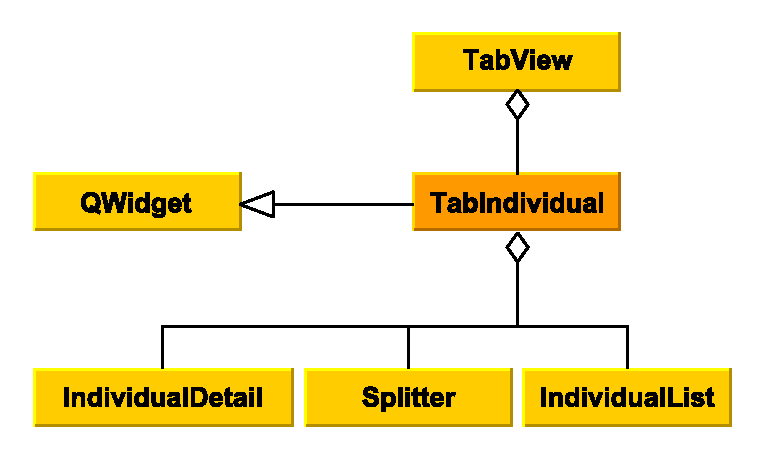
\includegraphics[width=9cm]{design/details/ui/tabIndividual.pdf}
			\caption{Třída \texttt{TabIndividual} a~její okolí}
			\label{fig:designDetailTabIndividual}
		\end{figure}
		Zobrazení je rozděleno na dvě poloviny. Na levé straně je zobrazen seznam všech evidovaných osob prostřednictvím tabulky \texttt{IndividualList}. Pravá strana potom zobrazuje editovatelná data o~vybrané osobě, tzv. probandovi. Šířka obou těchto zobrazení je uživatelsky nastavitelná prostřednictvím rozdělovače, nacházejícího se ve spojnici obou částí rozhraní. Jeho posunem se mění poměr plochy, zabrané zmíněnými objekty.\par
		Rozložení tohoto zobrazení i~složení objektů v~něm obsažených bylo inspirováno rozhraním českého programu Ancestry, popsaného v~sekci~\ref{sec:ance}. Jeho rozhraní so jisté míry splňovalo požadavky na rozhraní vytvářeného programu, proto bylo složení jeho rozhraní použito jako inspirace.\par
		
		\subsection*{Třída \texttt{IndividualList}}
		Odvozením od struktury pro vytváření tabulkových zobrazení vznikla třída obsahující seznam všech osob evidovaných v~editovaném rodokmenu. Struktura okolí této třídy je znázorněna v~obrázku~\ref{fig:designDetailIndividualList}.\par
		\begin{figure}[h]
			\centering
			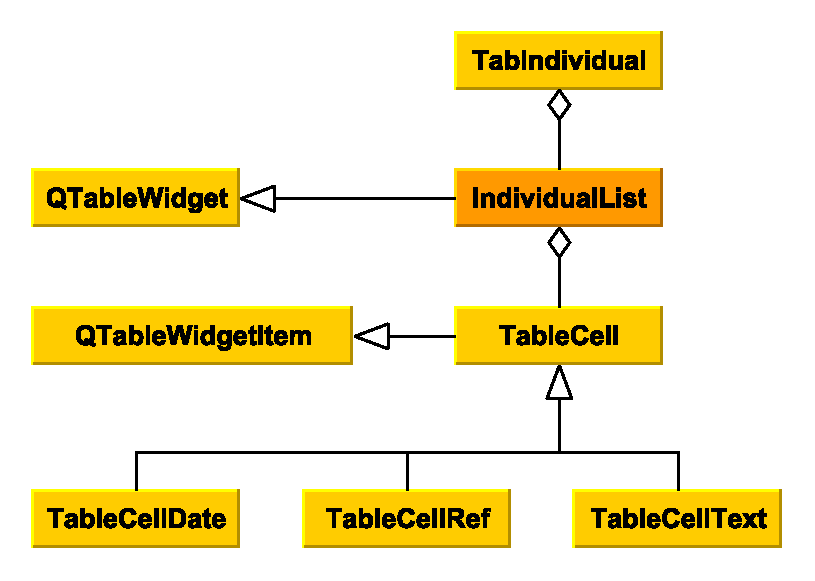
\includegraphics[width=10cm]{design/details/ui/individualList.pdf}
			\caption{Třída \texttt{IndividualList} a~její okolí}
			\label{fig:designDetailIndividualList}
		\end{figure}
		Přehled je aktuálně tvořen čtyřmi sloupci se základními údaji. Sloupce obsahují po řadě identifikátor osoby, jméno, příjmení a~rok narození. Základní řazení osob odpovídá pořadí jejich vložení do databáze. Další řazení je potom možné provádět kliknutím na vybraný sloupec. Záznamy jsou poté seřazeny sestupně dle hodnot. Řazení je kumulativní; v~případě totožných hodnot záleží pořadí záznamů na předchozím seřazeném sloupci nebo sloupcích.\par
		Výběrem záznamu o~osobě v~této tabulce se naplní zobrazení \texttt{IndividualDetail} daty této vybrané osoby. Kromě přehledu tedy tabulka umožňuje i~okamžitý přesun mezi osobami a~nabízí způsob, jak rychle procházet data u~zaznamenaných osob. \par
		
		\subsection*{Třída \texttt{IndividualDetail}}
		Třída \texttt{IndividualDetail} je jednou z~nejvýznamnějších struktur v~grafickém rozhraní. Odehrává se v~ní nejvyšší počet případů užití programu a~obsahuje zdaleka největší množství dat. Zjednodušený náhled okolí třídy je znázorněn v~obrázku~\ref{fig:designDetailIndividualDetail}.\par
		\begin{figure}[t!]
			\centering
			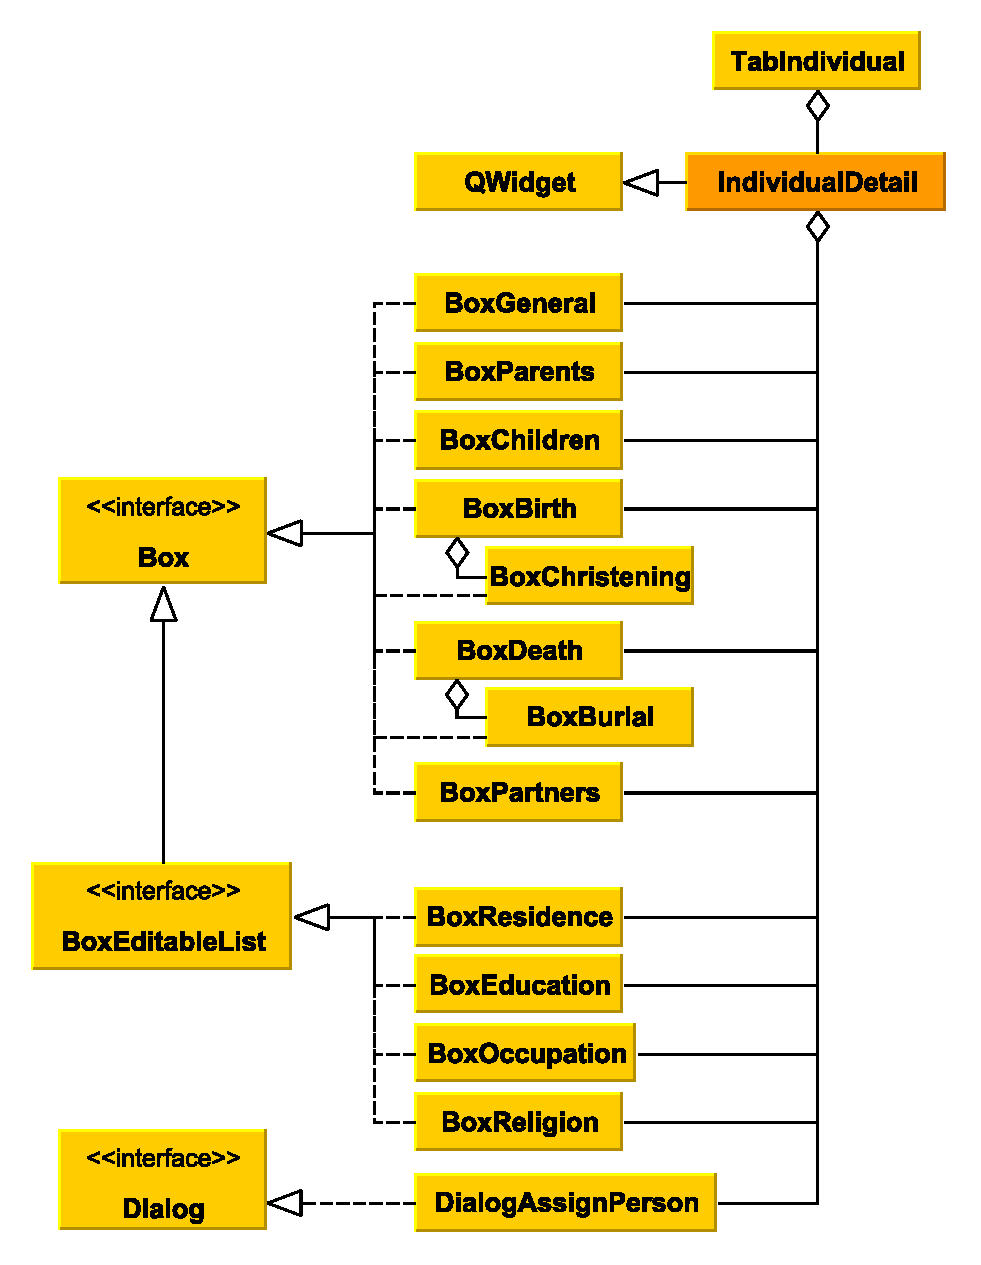
\includegraphics[width=12cm]{design/details/ui/individualDetail.pdf}
			\caption{Třída \texttt{IndividualDetail} a~její okolí}
			\label{fig:designDetailIndividualDetail}
		\end{figure}
		Návrh této třídy a~grafického rozložení jejího zobrazení byl jednou z~nejklíčovějších fází návrhu grafického uživatelského rozhraní. Obrazovka musela pojmout velké množství informací, a~přitom musela být zachována její přehlednost a~uživatelská přívětivost. Tyto požadavky vedly k~vytvoření struktury stavebnicového vzhledu. Jednotlivé bloky jsou popsány tučným nadpisem a~ohraničeny pro zvýšení přehlednosti. Tyto boxy jsou tvořeny instancemi tříd odvozených od třídy \texttt{Box}.\par
		Na první pohled je zřejmé, že zobrazení je prostorově rozčleněno do čtyř vertikálních skupin, které by se daly nazvat řádky. Každý z~těchto řádků zobrazuje skupinu dat, která spolu mají logické souvislosti. \par
		První řádek obsahuje základní informace o~osobě. Je zde box pro zaznamenání údajů jako jsou jméno, příjmení, pohlaví a~tituly osoby. Následuje box s~odkazy na rodiče prohlížené osoby. V~posledním boxu jsou potom zobrazeni sourozenci osoby. \par
		Další řádek obsahuje informace o~dvou základních milnících v~životě sledované osoby -- data týkající se jejího narození a~případného úmrtí. V~boxu pro zaznamenání narození je k~dispozici také prostor pro poznamenání detailů křtu, stejně jako je v~boxu zaznamenávajícím úmrtí osoby k~dispozici oddíl pro zanesení dat o~pohřbu.\par
		Ve třetím řádku jsou k~dispozici data související s~partnery dané osoby. Data jsou tříděna do záložek. První záložka je čistě přehledová a~jsou v~ní zaznamenány všichni potomci dané osoby, a~to včetně potomků, u~nichž chybí záznam o~druhém rodiči. Případné další záložky vyjadřují další partnery sledované osoby. Záložka partnera je nadepsána uživatelsky přívětivým řetězcem identifikujícím danou osobu. V~záložce jsou pak zobrazeny společné děti partnerů a~údaje o~případném sňatku a~rozvodu dvojice.\par
		Poslední řádek tohoto zobrazení má za úkol pojmout dodatečná data související s~osobou. Jsou zde čtyři boxy evidující záznamy o~místech bydliště, vzdělání, zaměstnáních a~náboženských vyznáních sledované osoby. Tyto záznamy jsou jako jediné přidávány a~editovány prostřednictvím vyskakovacího okna.\par
		Všechna ostatní data mohou být uživatelem editována přímo na místě. Při výběru osoby se kurzor objeví přímo v~poli se jménem osoby, s~editací je tedy možné začít jediným kliknutím, provádějícím výběr osoby. Posun na další pole je možné provést nejen interakcí prostřednictvím myši, ale i~stisknutím tabulátoru. Tato skutečnost dále přispívá ke svižnosti, s~jakou je uživatel schopen s~aplikací interagovat.\par
		Skutečnost, že jsou všechna data obsažena v~jediné obrazovce, umožňuje uživateli udržovat nad těmito daty přehled a~snižuje množství informací, které je uživatel nucen si pamatovat~\cite{bib:DesignUI}.\par
		
		\subsection*{Třída \texttt{TreeView}}
		Tato třída definuje záložku pro zobrazení stromu. Do budoucna také může být využita v~místech, kde je třeba vytvořit dočasný náhled stromu. Celá grafická plocha této struktury je naplněna objektem pro zobrazování grafických scén. \par
		Vytvoření stromového diagramu probíhá následovně. Nejprve uživatel zvolí druh diagramu z~nabídky programu. Na základě tohoto požadavku program zkonstruuje vybraný typ grafické scény. Scéna je posléze nastavena jako obsah tohoto zobrazení a~dojde k~přepnutí záložky tak, aby byl vykreslený diagram viditelný.\par
		Náhled této třídy je k~dispozici v~obrázku~\ref{fig:designDetailTreeView}.\par
		\begin{figure}[h]
			\centering
			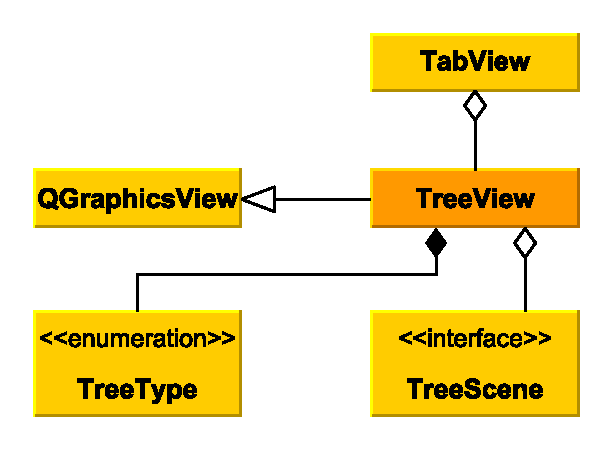
\includegraphics[width=7.5cm]{design/details/ui/treeView.pdf}
			\caption{Třída \texttt{TreeView} a~její okolí}
			\label{fig:designDetailTreeView}
		\end{figure}
		
		\subsection*{Dekorátor pro generování stromových scén}
		Generování stromových scén je řešeno za využití návrhového vzoru dekorátor. K~tomuto návrhovému rozhodnutí bylo přistoupeno z~toho důvodu, že vykreslování stromu je variabilní činnost, která se může drobně měnit na základě požadavků uživatele. Tento přístup k~návrhu umožňuje budoucí rozšíření generovaných stromů o~další druhy schémat i~o~uživatelsky zcela přizpůsobitelný diagram.\par
		Základní třída zaštiťující tvorbu stromové scény je třída \texttt{TreeScene}. Ta obsahuje deklarace čistě virtuálních metod využívaných odvozenými třídami. Tato třída je společně se svým okolím vyobrazena v~obrázku~\ref{fig:designDetailTreeScene}. \par
		\begin{figure}[h]
			\centering
			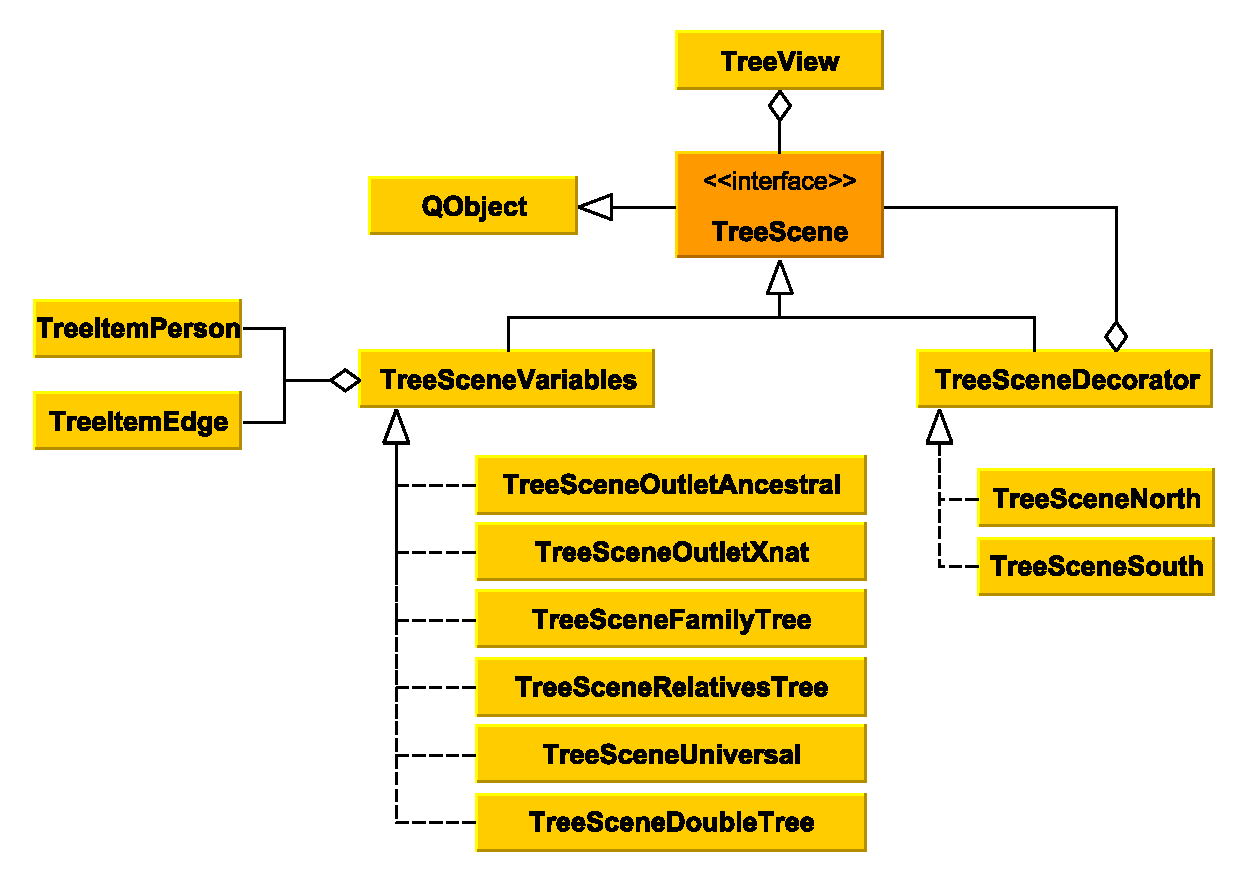
\includegraphics[width=15cm]{design/details/ui/treeScene.pdf}
			\caption{Třída \texttt{TreeScene} a~její okolí včetně dekorátorů}
			\label{fig:designDetailTreeScene}
		\end{figure}
		Tato třída má pouze dva přímé potomky odvozené jednoduchou dědičností. Jsou to třídy \texttt{TreeSceneVariables} a~\texttt{TreeSceneDecorator}. Jedná se o~virtuální bázové třídy, z~nichž jsou již odvozovány třídy implementující algoritmy konstrukce a~dekorování. První z~těchto tříd slouží k~deklarování čistě virtuálních metod zaměřených na konstruování stromu z~osob v~rodokmenu a~jejich rodinných svazků. Druhá třída zapouzdřuje ukazatel na zkonstruovaný strom. Přepsáním virtuálních metod této třídy je možné obsažený strom dekorovat. \par
		Od třídy \texttt{TreeSceneVariables} jsou jednoduchou dědičností odvozeny čtyři podtřídy. První z~nich je \texttt{TreeSceneFamilyTree}, která obsahuje implementaci metod pro konstrukci a~vykreslení diagramu rozrodu.  Další je třída \texttt{TreeSceneOutletAncestral}, která inicializuje a~vykresluje rodový vývod, a~od níž je odvozena podtřída \texttt{TreeSceneOutletXnat}, která přepisuje inicializační metodu tak, že je vytvořen pouze agnátní či kognátní vývod. Spojením tříd pro rozrod a~vývod vznikla třetí odvozená třída \texttt{TreeSceneRelativesTree}, která vykresluje kombinaci těchto dvou diagramů. \par
		Na podobném principu je založena i~poslední odvozená podtřída \texttt{TreeSceneDoubleTree}. Ta obsahuje ukazatele na dvě scény; jedna je míněna pro vykreslení do koruny, druhá pro vykreslení do kořenů stromového diagramu. Výběr konkrétních diagramů, které se vykreslí, je ale v~rukou uživatele. Skrze interakci s~touto třídou je tedy možné vykreslit například diagram, v~němž se do koruny rozvíjí agnátní a~go kořenů kognátní vývod, nebo například vykreslit strom příbuzenstva v~opačném směru tak, že v~koruně budou potomci a~v~kořenech předkové. Funkcionality této třídy zatím ovšem nejsou v~programu využity a~zpřístupněny koncovému uživateli grafického rozhraní, jedná se tedy spíše o~návrh směru vývoje, kterým by se aplikace mohla v~budoucnu vydávat.\par
		Oproti tomu od třídy \texttt{TreeSceneDecorator} jsou jednoduchou dědičností odvozeny pouze dvě třídy. Tyto třídy v~sobě zapouzdřují diagram, vygenerovaný pomocí některé ze tříd odvozených od \texttt{TreeSceneVariables} a~dekorují volané metody, tak, aby byl zajištěn vybraný směr vykreslení stromu. Jedná se o~třídu \texttt{TreeSceneNorth}, která slouží k~vykreslování diagramu do koruny, diagram je tedy větven od probanda směrem nahoru, a~analogicky o~třídu \texttt{TreeSceneSouth}, která diagram situuje do kořenů, diagram je tedy veden od probanda směrem dolů.\par
		Pokud je třída odvozená od \texttt{TreeSceneVariables} instanciována bez zapouzdření do některého z~dekorátorů, nebrání to její správné funkci. V~takovém případě je diagram vždy vykreslen směrem do koruny, rozvoj stromu tedy probíhá od probanda směrem nahoru.\par
		
		\subsection*{Obecný algoritmus pro vykreslování stromu}
		Zobecněná verze algoritmu pro vykreslení stromového diagramu probíhá v~instancích odvozených od třídy \texttt{TreeSceneVariables} a~to ve dvou fázích. V~první fázi jsou inicializovány objekty a~je vytvořeno jejich logické propojení do stromu. Ve druhé fázi jsou potom objekty rozmístěny na plochu a~je vytvořeno prostorové rozmístění scény.\par
		Inicializační fáze probíhá v~metodě \\ \texttt{initNodeTree}. \par 
		Vstupním parametrem je výchozí osoba schématu a~číslo aktuálně inicializované generace, které je u~počátečního volání rovno nule.\par
		U~vstupní osoby potom začíná činnost samotného algoritmu. Osoba je analyzována a~jsou identifikovány vztahy, které jsou pro diagram klíčové (např. rodiče u~diagramu typu rodový vývod). Jsou získány identifikátory všech takových osob, a~poté jsou tyto identifikátory předány do rekurzivního volání inicializační funkce, společně s~hodnotou počítadla generací povýšenou o~jedna. Z~těchto volání jsou navráceny ukazatele na zkonstruované buňky těchto osob. \par
		Poté následuje konstrukce buňky vstupní osoby a~její uložení do vnitřní paměti instance. Nově vytvořená buňka je poté propojena s~dříve získanými ukazateli na buňky souvisejících osob a~dojde tak k~vytvoření stromových vztahů mezi buňkami. Činnost je završena inicializací shluku hran, které výchozí buňku propojují s~buňkami, k~nimž má vztah. \par
		Zanořování rekurzivního volání je ukončeno tehdy, je-li metodě předán neplatný identifikátor osoby. K~tomu dochází zpravidla tehdy, není-li osoba sledovaným vztahem vázána k~žádné jiné evidované osobě. V~takovém případě metoda vrátí nulu.\par
		Po dokončení inicializace následuje fáze rozmisťování objektů na plochu. K~distribuci objektů dochází v~metodě \texttt{drawNodeTree}. Parametry jsou tentokrát tvořeny buňkou, zachycující výchozí osobu, a~číslem aktuálně vykreslované generace, která je u~počátečního volání metody rovna nule. \par 
		Vykreslení buněk probíhá dle průchodu zkonstruovaným stromem podle algoritmu Post-order. Nejprve jsou rekurzivním voláním metody vykresleny všechny buňky, k~nimž má výchozí buňka vztah. Poté dochází k~polohování výchozí buňky. \par
		Buňka je vertikálně posunuta tak, aby se nacházela v~úrovni vhodné pro svou generaci. Poté probíhá horizontální umístění buňky. Pokud buňka nemá žádné platné vazby, je umístěna na nejlevější dostupnou pozici. V~opačném případě je spočítána souřadnice, kde se nachází středová pozice buněk, k~nimž má výchozí buňka vazby. Výchozí buňka je poté napolohována do získané pozice. Tímto krokem je dokončeno základní polohování. \par
		Dále je nutno provést kontrolu, zda vykreslením buňky na určené pozici nedojde k~překrytí již umístěných objektů. Pokud je tento problém identifikován, je buňka společně se všemi buňkami, k~nimž má vztah, posunuta tak, aby k~překrytí nedocházelo. \par
		Jakmile je potvrzeno, že je umístění buňky validní a~nevede ke kolizím s~ostatními objekty, je buňka vložena do scény. \par
		Polohování buněk je prováděno vždy tímtéž směrem, a~to do kořenů stromu. Pro změnu tohoto výchozího způsobu polohování je nutné vykreslovanou instanci zapouzdřit v~příslušném dekorátoru.\par
		Po vynoření z~rekurze a~dokončení algoritmu vykreslení je vytvořena kompletní scéna s~rodovým schématem. Buňky v~takové scéně jsou rozmístěny tak, že je její prostor využit na maximum. Šířku diagramu již nelze zúžit, aniž by došlo k~překryvu buněk či porušení jejich minimálních rozestupů, totéž platí pro výšku diagramu.\par 
		
		\subsection*{Dekorátory pro objekty ve stromě}
		Stromová scéna je tvořena dvěma základními druhy objektů. Prvním jsou buňky s~údaji o~jednotlivých osobách, reprezentované třídou \texttt{TreeItemPerson} a~druhým jsou shluky kolmých hran, propojující související buňky do diagramu, tvořené definované třídou\\ \texttt{TreeItemEdge}. Obě tyto struktury a~jejich okolí jsou znázorněny v~obrázku \ref{fig:designDetailTreeItem}. \par
		\begin{figure}[h]
			\centering
			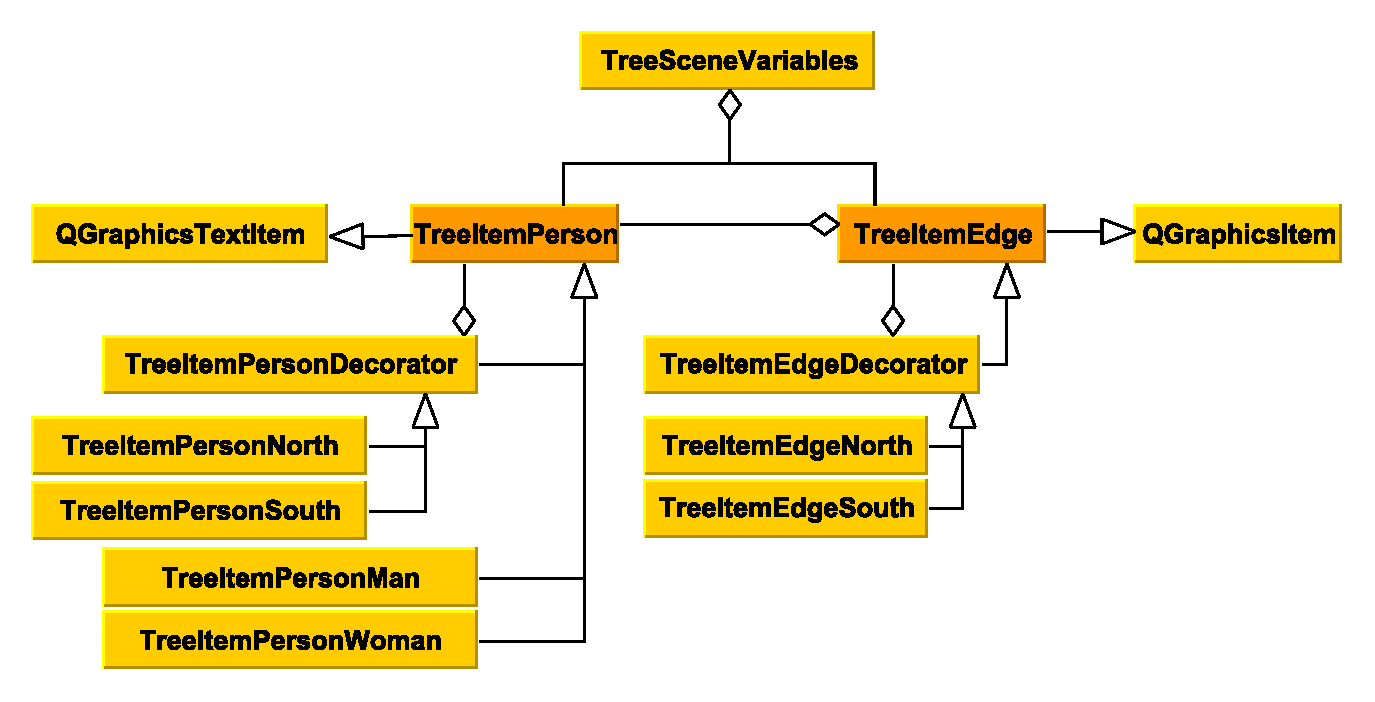
\includegraphics[width=15cm]{design/details/ui/treeItem.pdf}
			\caption{Třídy \texttt{TreeItemPerson} a~\texttt{TreeItemEgde} a~jejich okolí včetně dekorátorů}
			\label{fig:designDetailTreeItem}
		\end{figure}
		Základní objekt, od něhož jsou odvozeny všechny třídy definující buňky v~diagramu, je třída \texttt{TreeItemPerson}. Jednoduchou dědičností jsou od ní odvozeny tři třídy. První dvojice těchto podtříd jsou \texttt{TreeItemPersonMan} a~\texttt{TreeItemPersonWoman}. Tyto třídy upravují tvar rámečku u~osob po řadě mužského a~ženského pohlaví. U~mužů je tvar rámečku zachován v~podobě s~ostrými hranami, u~žen jsou hrany rámečku zakulaceny.\par
		Další přímo odvozenou podtřídou je třída \texttt{TreeItemPersonDecorator}. Jak již vyplývá z~jejího názvu, jedná se o~dekorátor. Zapouzdřuje v~sobě ukazatel na zkonstruovanou buňku, kterou je možné dekorovat přepsáním virtuálních metod této třídy.\par
		Od třídy dekorátoru jsou odvozeny podtřídy \texttt{TreeItemPersonDecoratorNorth} \\a \texttt{TreeItemPersonDecoratorSouth}. Tyto podtřídy upravují metody pro nastavování a~navracení souřadnic tak, aby se buňky vykreslily do správné části plochy dle určeného směru vykreslování diagramu. \par
		Dalším základním objektem, vykreslovaným do plochy scény, je objekt zachycující spojnici buněk. Ten je definován základní třídou \texttt{TreeItemEdge}, která v~sobě zapouzdřuje shluk hran, které tvoří spojnici mezi výchozí buňkou a~buňkami o~generaci posunutými, k~nimž má výchozí buňka definovaný vztah.\par
		Od této třídy je prostou dědičností odvozena pouze třída vytvářející bázi pro dekorátory, třída \texttt{TreeItemEdgeDecorator}. Tato třída opět obaluje ukazatel na instanci zkonstruovaného shluku hran.
		I~třída pro spojnice může být upravena dvěma typy dekorátoru, \texttt{TreeItemEdgeDecoratorNorth} a~\texttt{TreeItemEdgeDecoratorSouth}. V~těchto třídách jsou opět upraveny metody, jejichž zodpovědnosti souvisí s~polohováním hran v~prostoru, a~to tak, aby výsledné polohy hran odpovídaly určenému směru vykreslování.\par	
		
		\subsection*{Třída \texttt{TabSource}}
		Třída \texttt{TabSource} se zabývá správou prostorového rozložení objektů zobrazovaných v~záložce se zdroji. Obrazovka této záložky sestává ze dvou polovin oddělených rozdělovačem, jehož poloha je uživatelsky nastavitelná. Uživatel tedy může upravovat vzájemný šířkový poměr zobrazovaných objektů. Třída a~její nejbližší okolí je znázorněna v~obrázku \ref{fig:designDetailTabSource}.\par
		\begin{figure}[h]
			\centering
			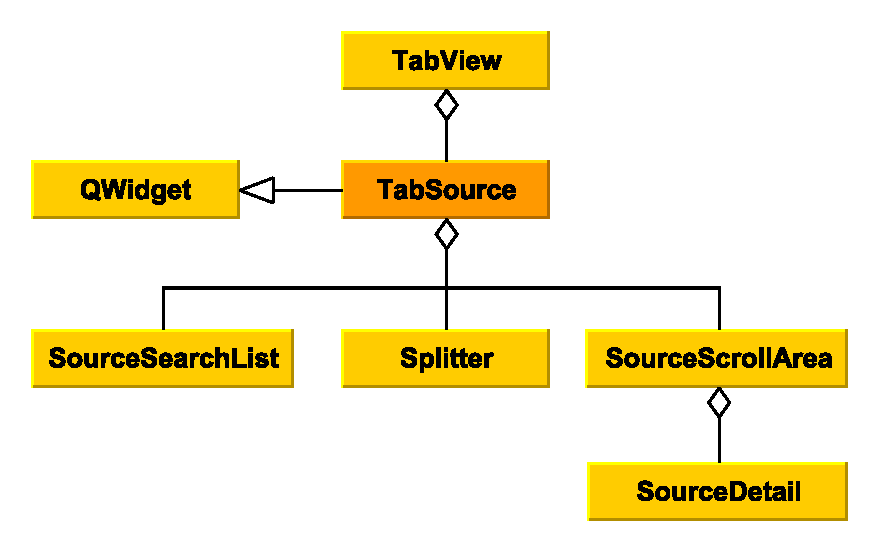
\includegraphics[width=10cm]{design/details/ui/tabSource.pdf}
			\caption{Třída \texttt{TabSource} a~její okolí}
			\label{fig:designDetailTabSource}
		\end{figure}
		V~levé polovině záložky je zobrazena instance třídy \texttt{SourceSearchList}, která uživateli umožňuje vyhledání zdroje a~jeho výběr pro následnou editaci v~pravé straně zobrazení. Tam je v~rolovatelném zobrazení vložena instance třídy \texttt{Source Detail}, zobrazující editovatelné detaily vybraného zdroje. Není-li žádný zdroj vybraný, je tato část zobrazení prázdná.\par
		Jelikož nebyl identifikován žádný program, který by zaznamenával zdroje akceptovatelným způsobem, odpovídajícím požadavkům na tento program, byl návrh této časti rozhraní i~objektů v~něm obsažených proveden do nuly. \par
		
		\subsection*{Třída \texttt{SourceSearchList}}
		V~rámci třídy \texttt{SourceSearchList} je navrženo grafické rozhraní pro přehledné zobrazení evidovaných zdrojů. Záznamy o~zdrojích jsou zobrazeny v~seznamu. Zobrazené vstupy je možné filtrovat prostřednictvím zadání uživatelského vstupu do textového pole umístěného nad seznamem. Dále je v~pravém horním rohu objektu k~dispozici dvojice tlačítek. První z~nich slouží pro přidávání zdroje, druhé z~nich umožňuje odstraňování zdrojů. \par
		
		\subsection*{Třída \texttt{SourceDetail}}
		Tato třída zapouzdřuje objekty vytvářející zobrazení pro úpravu detailů vybraného zdroje, jak je znázorněno v~obrázku \ref{fig:designDetailSourceDetail}. Při vkládání do rodičovského objektu je instance této třídy vložena do rolovatelného zobrazení, aby při vložení velkého počtu záznamů nedošlo k~přetečení objektu mimo hranice obrazovky programu. \par
		\begin{figure}[h]
			\centering
			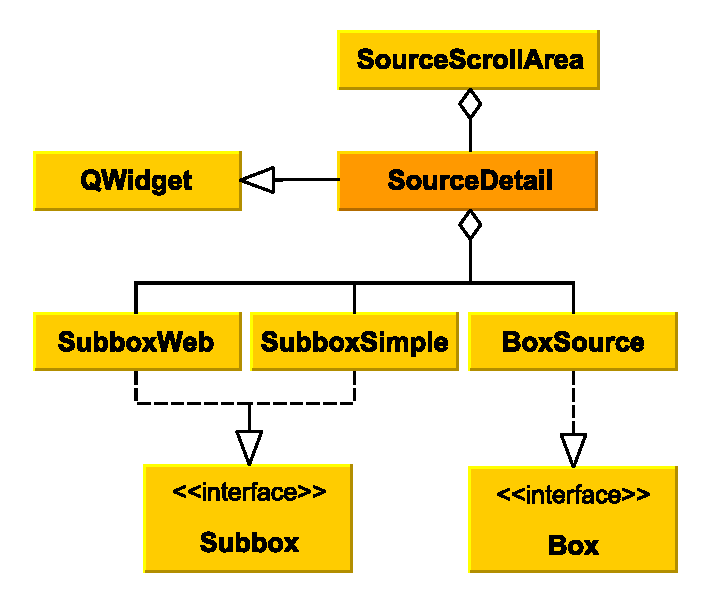
\includegraphics[width=8cm]{design/details/ui/sourceDetail.pdf}
			\caption{Třída \texttt{SourceDetail} a~její okolí}
			\label{fig:designDetailSourceDetail}
		\end{figure}
		Zobrazení je rozděleno na čtyři sekce umístěné ve vertikálním rozložení. První sekce, která se nachází v~horní části zobrazení, zaznamenává základní informace o~zdroji jako celku. Jsou zde uloženy informace o~matriční knize jako celku, tedy název archivu, který knihu spravuje, signatura matriční knihy, původce matriky a~webová adresa odkazující na digitalizovanou matriku.\par
		Následují tři analogické sekce, archivující data o~záznamech, obsažených v~matrice. Sekce jsou děleny dle typu zaznamenávané události na oddíl obsahující detaily záznamů o~narození, na oddíl shromažďující data o~záznamech o~sňatku a~na závěr na oddíl pro zapsání dat o~záznamech o~úmrtí. Všechny tyto sekce přitom sdílí totéž grafické rozložení obsažených komponent.\par
		Pod nadpisem boxu se nachází tlačítko pro přidání dat o~novém záznamu daného typu. Takový záznam sestává z~polí pro místo, evidované časové období, rozsah stran, na nichž jsou v~matrice tyto záznamy dostupné a~odkaz na digitalizovanou matriku. Přidáním více záznamů vznikne struktura, připomínající tabulku, kde první řádek slouží jako nadpis sloupců a~každý další řádek reprezentuje jeden evidovaný zápis o~záznamu. Každý z~těchto evidovaných zápisů je možné odstranit pomocí tlačítka, které je umístěno vždy v~nejpravějším sloupci strukturovaného zobrazení.\par
		
		\subsection*{Třída \texttt{TabStatistics}}
		Třída \texttt{TabStatistics} je návrh třídy, sloužící pro zobrazení záložky s~rodovými statistikami. Třída aktuálně není použita, ale slouží spíše jako základ pro rozvinutí budoucích statistických funkcionalit.\par
		V~současné podobě je třída odvozena od bázové třídy pro editaci textu. Toto textové pole je uzamčeno proti uživatelské editaci. Výpis je aktuálně prováděn do tohoto pole v~podobě strukturovaného textu. Uživatel tento text může zkopírovat do schránky a~dále jej využít např. pro účely kroniky.\par
		Funkcionalita statistik je výhodná také z~pohledu kontroly zadaných dat. Při zobrazení neočekáváných extrémních hodnot ve statistikách může uživatel odhalit chyby ve svých datech, které by jinak mohl přehlédnout.\par
		
		\subsection*{Třída \texttt{Box} a~třídy od ní odvozené}
		Třída \texttt{Box} je bázovou třídou pro celou řadu klíčových tříd, které zastávají důležité funkce v~uživatelském rozhraní. Třídy odvozené od této báze jsou vizuálně na první pohled rozpoznatelné podle toho, že se jedná o~objekty, obalující skupinu komponent do tučně nadepsaného boxu obaleného rámečkem. Rozhraní \texttt{Box} a~jeho okolí je znázorněno v~obrázku \ref{fig:designDetailBox}. \par
		\begin{figure}[h]
			\centering
			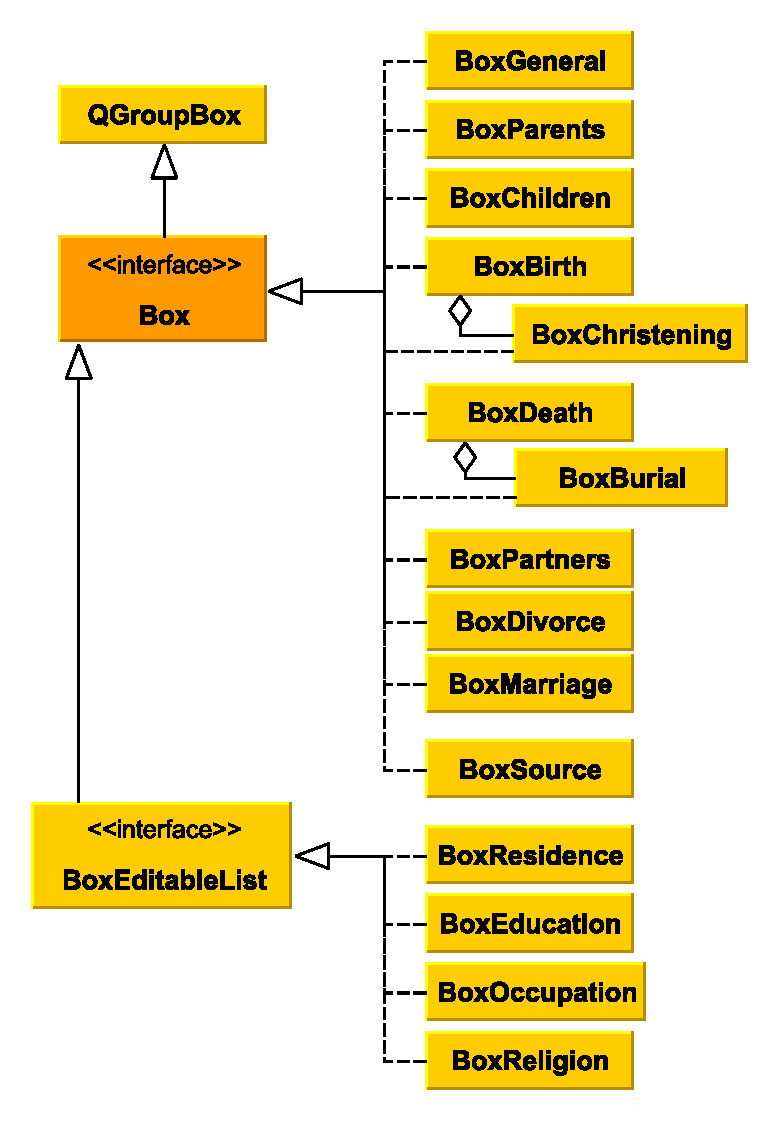
\includegraphics[width=10cm]{design/details/ui/box.pdf}
			\caption{Třída \texttt{Box} a~její okolí}
			\label{fig:designDetailBox}
		\end{figure}
		Jsou to téměř výhradně objekty odvozené od této třídy, které tvoří zobrazení detailu osoby ve třídě \texttt{IndividualDetail}. Odvozené objekty jsou ale použity např. i~pro boxy evidující záznamy konkrétního typu u~zdrojů.\par
		V~kontextu této třídy stojí za zmínku její konstruktor. Ten obsahuje celou řadu parametrů. Specifické jsou první dva z~nich. První slouží k~nastavení titulku, zobrazovaného nad boxem. Další parametr zase určuje, zda je v~levém horním rohu objektu zobrazen box pro zaškrtnutí. Tato funkcionalita je využívána např. u~boxu evidujícího data o~úmrtí či u~boxu zaznamenávajícího sňatek, jelikož se jedná o~události, které u~dané osoby či páru nemusely nastat.\par
		Bázová třída vytváří základ pro rozložení komponent uvnitř objektu a~deklaruje několik čistě virtuálních metod, které jsou použity pro inicializaci a~aktualizaci odvozených objektů. Také jsou zde definovány konstantní podoby opakujících se textových řetězců a~sdílené rozhraní v~podobě signálu notifikujícího o~změně probanda.\par
		
		\subsection*{Třída \texttt{Subbox} a~třídy od ní odvozené}
		Je patrné, že celá řada prvků uživatelského rozhraní, např. oddíl pro zadávání data události, se často opakuje. Tyto prvky jsou navrženy jako instance tříd, odvozených od bázové třídy \texttt{Subbox}. Narozdíl od tříd odvozených od výše zmíněné třídy \texttt{Box} tyto prvky nejsou nijak vizuálně specifické a~nelze je tedy při pohledu na rozhraní jediným pohledem rozpoznat. Diagram znázorňující rozhraní \texttt{Subbox} a~jeho nejbližší okolí je znázorněn na obrázku \ref{fig:designDetailSubbox}.\par
		\begin{figure}[h]
			\centering
			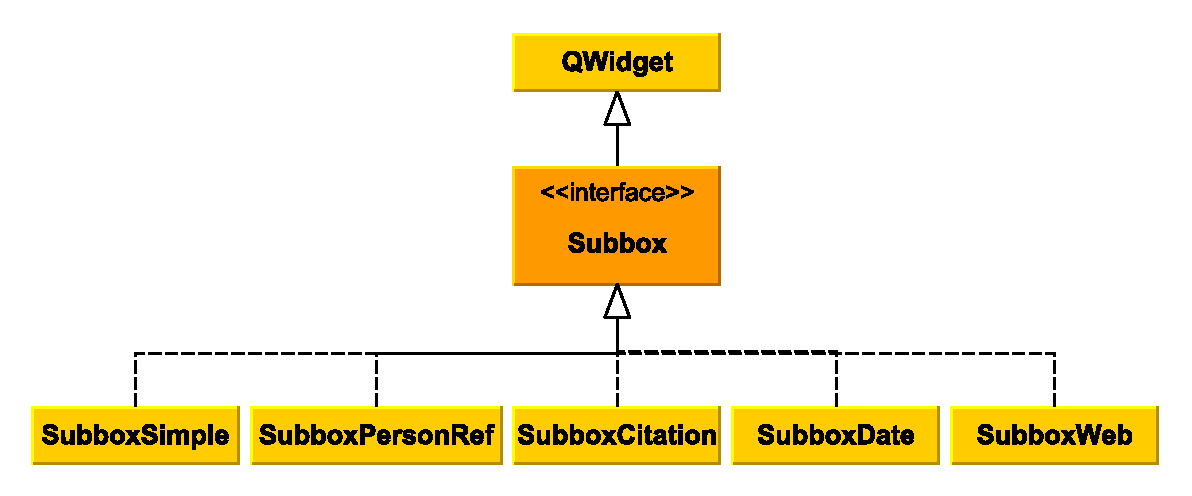
\includegraphics[width=15cm]{design/details/ui/subbox.pdf}
			\caption{Třída \texttt{Subbox} a~její okolí}
			\label{fig:designDetailSubbox}
		\end{figure}
		Patří mezi ně již zmíněné pole pro zadávání data, ale též pole pro uložení místa události, pole pro vybrání související osoby, pole pro zaznamenání odkazu na web či pole pro zadávání citací použitých zdrojů.\par
		Rodičovská třída tohoto typu poskytuje odvozeným objektům jednotný přístup k~tvorbě rozložení a~deklaruje čistě virtuální metodu určenou pro inicializaci objektu.\par
		Za zmínku zde stojí především odvozená podtřída \texttt{SubboxWeb}. Ta obsahuje pole pro uložení odkazu na webovou stránku, doplněné o~tlačítko, které danou stránku otevře v~nové záložce výchozího prohlížeče. Tato komponenta tak umožňuje velmi rychlou interakci s~programem a~jeho propojení s~digitalizovanými zdroji je ještě pevnější.\par
		
		\subsection*{Třída \texttt{Dialog} a~třídy od ní odvozené}
		Třída \texttt{Dialog} zaštiťuje velkou část objektů rozšiřujících základní uživatelské rozhraní. Jedná se o~objekty, zobrazující se v~modálním okně plovoucím nad hlavním oknem uživatelského rozhraní. \par
		Tato bázová třída zajišťuje jednotný vzhled všech modálních oken aplikace. Je skryto tlačítko pro zobrazení nápovědy a~nastaveno jednotné rozložení obsahu okna. Třída také deklaruje čistě virtuální metodu pro inicializaci komponent okna.\par
		Jak ilistruje obrázek \ref{fig:designDetailDialog}, dialogy zobrazované aplikací se dělí do několika kategorií. První z~nich je kategorie dialogů sloužících pro načítání a~ukládání souborů. Tato skupina je specifická především tím, že jako jediná nedědí od výše zmíněné bázové třídy.\par
		\begin{figure}[h]
			\centering
			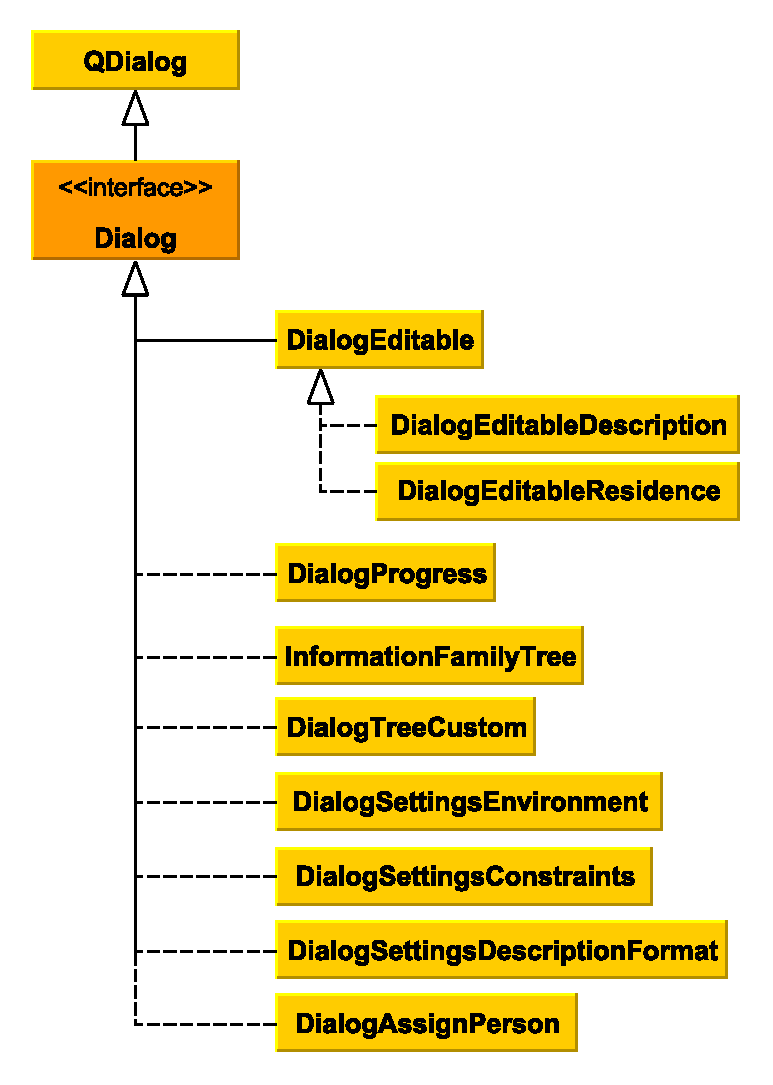
\includegraphics[width=10cm]{design/details/ui/dialog.pdf}
			\caption{Třída \texttt{Dialog} a~její okolí}
			\label{fig:designDetailDialog}
		\end{figure}
		Další kategorie je tvořena dialogy, které mají přímý vliv na úpravu dat. Prvním dialogem z~této skupiny, který určitě stojí za zmínku, je dialog \texttt{DialogAssignPerson}, vyvolávaný při požadavku na přiřazení nového odkazu na osobu. Ten uživateli nabízí výběr ze seznamu platných osob, doplněný o~možnost vytvoření osoby nové. Nabídnuté osoby je navíc možné pro lepší přehlednost filtrovat pomocí textového vstupu do pole nad seznamem.\par
		Další dialog z~této kategorie, \texttt{DialogEditable}, je virtuální bázovou třídou pro dialogy editující a~přidávající data o~bydlišti osoby, vzdělání apod. Dialog vytváří sdílené rozhraní pro předávání data a~jsou od něj odvozeny dvě třídy specifikující konkrétní rozložení komponent v~dialogu a~doplňující rozhraní tak, aby byla předávána i~ostatní evidovaná data.\par
		Posledním dialogem z~této skupiny je \texttt{DialogFamilyTree}. Jedná se o~jednoduchý dialog sloužící k~zaznamenání základních údajů o~genealogickém projektu, jako je jméno jeho autora či datum vytvoření. Je v~něm také prostor na další poznámky k~rodokmenu.\par
		Další kategorie zahrnuje jediný dialog. Je jím dialog zprostředkovávající uživateli informace o~průběhu importu souboru prostřednictvím ukazatele průběhu. Jedná se o~jednoduchý modální dialog, který neumožňuje uživatelskou interakci a~automaticky zmizí po skončení importu.\par
		Další kategorie souvisí s~vykreslováním stromových diagramů a~opět zahrnuje jediný dialog. Jedná se o~dialog \texttt{DialogTreeCustom}. Jeho cílem je dodat uživateli grafické rozhraní k~nastavení vlastního vzhledu generovaného diagramu. Jelikož je tato vykreslovací funkcionalita v~současné době stále pouze experimentální součástí programu a~jejím hlavním cílem je nabídnout možný směr dalšího vývoje, není tento dialog aktuálně skrze uživatelské rozhraní zobrazitelný.\par
		Následující kategorie v~sobě zaštiťuje dialogy pro provádění uživatelských nastavení. Jedná se o~obyčejné objekty, které uživateli zprostředkovávají grafické rozhraní pro provedení nastavení souvisejících s~chováním a~zobrazováním programu.\par
		
		\subsection*{Třída \texttt{MessageBox} a~třídy od ní odvozené}
		Instance třídy \texttt{MessageBox} a~tříd od ní odvozených slouží primárně pro zvýšení uživatelské přívětivosti rozhraní. Tato třída je speciálním případem dialogu, který podává uživateli zprávu či varování související se stavem programu, zadanými daty či uživatelským požadavkem, a~dává tak uživateli přehled o~stavu aplikace případně předchází chybám. Třída a~od ní odvozené podtřídy jsou znázorněny v~obrázku \ref{fig:designDetailMessageBox}.\par
		\begin{figure}[h]
			\centering
			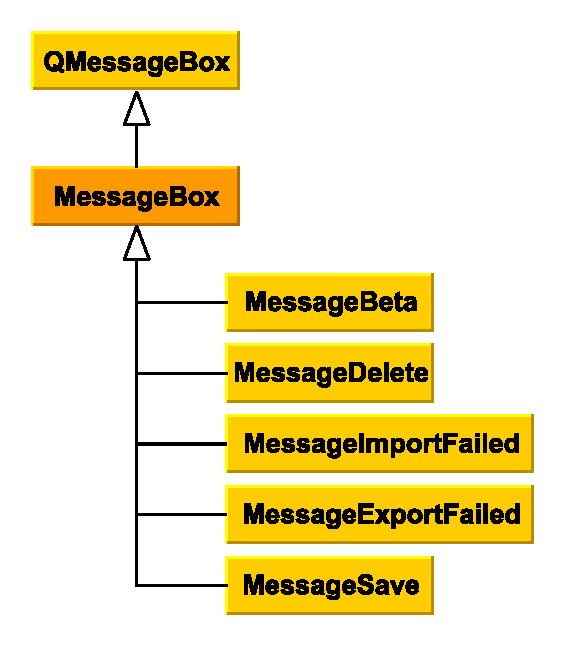
\includegraphics[width=7cm]{design/details/ui/messageBox.pdf}
			\caption{Třída \texttt{MessageBox} a~její okolí}
			\label{fig:designDetailMessageBox}
		\end{figure}
		Jedním z~nejdůležitějších dialogů, odvozených od této třídy, je dialog \texttt{MessageDelete}. Ten se zobrazí vždy, když se uživatel pokusí o~smazání dat, a~vyzve uživatele k~potvrzení či zamítnutí jeho volby. Slouží tedy jako prevence nechtěného odstranění záznamů.\par
		Dalším důležitým dialogem z~této kategorie je dialog \texttt{MessageSave}. Ten při zavírání programu či načítání nového souboru na úkor toho aktuálně otevřeného, vyzve uživatele, zda stojí o~uložení změn v~aktuálně spravovaném souboru. Kromě možností Ano a~Ne je uživateli nabídnuta volba Zrušit, která vede k~zastavení akce, jež zprávu vyvolala, a~editovaný soubor zůstane i~nadále otevřen.\par
		
		\subsection*{Možnosti nastavení programu}
		Program si perzistentně uchovává celou řadu hodnot v~podobě nastavení. K~jejich správě je použita platformě nezávislá třída \texttt{QSettings}. Některá z~těchto dat jsou přímo editovatelná uživateli, jiná jsou před uživateli skryta a~jsou zpracovávána programem na pozadí.\par
		Mezi uživatelem editovatelné hodnoty patří například údaj o~jazyku prostředí aplikace, hodnoty řetězců definujících formát textových výstupů nebo nastavení logického chování programu ve vztahu k~datům. Tato nastavení jsou uživateli zpřístupněna prostřednictvím série výše popsaných dialogů.\par
		Nastavení, jež jsou před uživatelem skryta, se týkají především rozložení uživatelského rozhraní. Program si z~posledního spuštění pamatuje velikost a~stav okna, šířku nastavitelných částí rozhraní, šířku jednotlivých sloupců v~seznamu osob či seznam posledních pěti úspěšně načtených souborů.\par
		
		\subsection*{Další zajímavé komponenty}
		Uživatelské rozhraní aplikace stojí kromě výše zmíněných tříd i~na celé řadě doplňkových objektů, které definují dodatečné komponenty nebo upravují výsledný vzhled či rozložení programu. Tři nejzajímavější budou popsány v~následujících odstavcích.\par
		První z~nich je virtuální třída \texttt{LabelWidthAdjuster}. Ta řeší problém vyvstávající z~používání objektů definovaných třídou \texttt{Subbox}. Použitím těchto objektů je znemožněno použití automatického rozložení komponent do mřížky. Docházelo by tak k~nestejnoměrnému zarovnání titulků na jednotlivých řádcích.\par
		Tato třída deklaruje dvě čistě virtuální metody, z~nichž jedna navrací maximální z~šířek všech popisků a~druhá tuto šířku nastavuje pro všechny tyto štítky. Poslední metodou je nevirtuální veřejná metoda, která postupně volá tyto virtuální členy a~zajišťuje tak rovnoměrné a~zarovnané rozložení výsledného zobrazení.\par
		Správné použití této třídy sestává ze tří fází. Nejprve musí být u~podtřídy deklarována dědičnost této báze, která je zpravidla doplněna vícenásobnou dědičností od třídy nějakého grafického objektu. Dále musí dojít k~validní implementaci virtuálních metod, která splňuje jejich specifikaci. Poslední fáze spočívá ve volání veřejné metody, která provede úpravu šířek. Důležité je provést toto volání až po inicializaci všech klíčových komponent.\par
		Druhá zajímavá třída je třída \texttt{DateValidator}. Ta slouží k~validaci platnosti uživatelem zadaného data. Datum je zadáváno prostřednictvím obyčejného textového pole, které narozdíl od dedikovaného pole na zadávání data zrychluje interakci s~programem. Vzhledem k~použití takové komponenty je ale nutné uživatelský vstup kontrolovat. Kontrola probíhá právě prostřednictvím instance této třídy, která je k~editovatelnému poli připojena.\par
		Kontrola vstupu může dopadnout dvěma způsoby. Ideálního stavu je dosaženo ve chvíli, kdy datum odpovídá stanovenému formátu a~je akceptováno. Druhá alternativa potom zahrnuje všechny neplatné vstupy.\par
		Třída je definována tak, že jako vstup přijímá pouze čísla a~oddělovače v~podobě tečky. Počet zadaných teček navíc nesmí překročit dva výskyty. Jakýkoliv vstup porušující tato pravidla je třídou eliminován.\par
		Poslední zajímavou komponentou je virtuální třída \texttt{List}. Tato třída je odvozena od objektu pro grafickou reprezentaci seznamů a~slouží jako báze pro objekty zobrazující seznamy osob a~zdrojů.\par
		Třída deklaruje čistě virtuální metodu pro vytvoření objektu v~seznamu na základě dodaného identifikátoru. Tato metoda je volána uvnitř metody pro aktualizaci obsahu seznamu, jejímž parametrem je právě vektor identifikátorů. Třída také nabízí celou řadu signálů a~slotů, umožňujících po řadě předání informace o~vybrané hodnotě a~filtrování dat v~seznamu na základě uživatelem zadaného textu.\par
		
		\subsection*{Třída \texttt{TextFormatter}}
		Jedná se o~statickou třídu sloužící pro generování uživatelsky příjemných textových výstupů z~dat uložených v~jádru. Konstruktor této třídy je privátní a~všechny metody, které nabízí, jsou statické. Třída tedy neslouží k~instanciování, ale pouze jako objekt zaštiťující skupinu metod podobného rázu.\par
		Přínos této třídy spočívá v~automatickém tvoření lidsky srozumitelných řetězců na základě definovaného formátu. Výsledný formát, v~jakém budou data v~aplikaci vypisována, je navíc plně v~pravomoci uživatele. \par
		Uživatel si může nadefinovat, jaká data budou vypisována u~jmen osob, zdrojů, jejich citací, i~buněk ve stromě. Data jsou reprezentována textovými parametry, které mohou být doplněny o~jakýkoliv uživatelský text. V~případě nastavení buněk stromového zobrazení je navíc možné obohatit definici prostřednictvím HTML značek i~o~formátování.\par

%===============================================================================
% Implementace aplikace
%===============================================================================

\chapter{Implementace aplikace}
\label{chap:implem}
Program \emph{ProGenealogy} byl implementován v~jazyce C++17 za využití frameworku Qt verze 5.12.3~\cite{bib:QtFramework}. Framework Qt byl vybrán nejen jako prostředník pro tvorbu uživatelského rozhraní, ale byly využity i~struktury pro správu specifických dat a~perzistentních nastavení. Kombinace jazyka C++ a~zmíněného frameworku byla vybrána mimo jiné i~za účelem zachování přenositelnosti implementovaného programu. Díky této vlastnosti může program zaujmout větší počet uživatelů, než kdyby byl striktně vyvíjen pro jedinou platformu \par
Při implementaci byla dále využita knihovna cgGedcom od Charlese Glancyho~\cite{bib:LibCgGedcom}. Tato knihovna poskytuje jednoduché rozhraní pro načtení souboru, vyhovujícího standardu GEDCOM, a~pro přístup k~jednotlivým strukturám a~jejich datům. Velkou předností této knihovny je také skutečnost, že hodnota značek není formalizována, je tedy možné pracovat i~se značkami, které byly do formátu uměle přidány. \par
Vývoj jádra aplikace proběhl na základě vodopádového modelu. Nejprve byl vytvořen návrh, na jehož základě potom byla implementována navržená funkcionalita. \par
Uživatelské rozhraní aplikace bylo vytvářeno za použití spirálového modelu. Nejprve bylo navrženo uživatelské rozhraní pro výběr a~editaci osoby s~nejzákladnějšími funkcionalitami. Rozhraní bylo postupně rozšiřováno o~pokročilejší funkce. Poté došlo k~návrhu a~implementaci algoritmů pro vykreslování stromů a~jejich zahrnutí do uživatelského rozhraní. Dále byly navrženy a~implementovány funkcionality související se správou zdrojů a~funkcionality byly i~nadále iterativně vylepšovány a~upravovány.\par
Důležitou součástí implementace aplikace bylo zahrnutí překladů do přirozených jazyků. Uživatelské rozhraní aplikace je v~nativní podobě v~anglickém jazyce. Pro jeho překlad bylo využito funkcionalit frameworku Qt pro internacionalizaci a~lokalizaci. Byly vygenerovány soubory s~textovými řetězci určenými k~překladu. Překlad byl poté proveden za využití programu Linguist, který je dodáván společně s~ostatním Qt softwarem. Aktuálně je dokončen úplný překlad do českého jazyka. Aplikace je tedy v~současné době dostupná ve dvou jazykových mutacích.\par
Pro uložení souborů s~překlady, stejně jako pro zapouzdření obrázků ikon a~tlačítek, byl použit Qt systém zdrojů. Ten umožňuje jednoduchou správu souborů souvisejících s~programem a~jejich zakomponování do výsledného binárního souboru. \par
Převážná část vývoje aplikace probíhala na 64bitové verzi operačního systému Windows 10 Education, s~občasným vyzkoušením na 64bitovém Ubuntu 18.04 LTS. Aplikace v~současné době funguje bezproblémově na obou zmíněných systémech a~díky podpoře přenositelnosti frameworkem Qt by aplikace měla fungovat i~na operačních systémech MacOS.\par
Aby byly naplněny požadavky na vytvoření open source aplikace, byly zdrojové kódy zveřejněny v~repozitáři na službě Atlassian Bitbucket. Odkaz na veřejný repozitář je k~nalezení na přiloženém disku v~souboru readme.txt, více informací v~příloze \ref{append:cd}. 

	\section{Výsledný vzhled uživatelského rozhraní aplikace}
	Výsledná aplikace sestává ze čtyř záložek, které uživateli zprostředkovávají všechny základní případy užití. Jedná se o~záložky zobrazující osobu a~poznámky k~osobě, o~záložku zobrazující strom, a~nakonec o~záložku pro správu zdrojů.\par
		\subsection*{Výsledný vzhled rozhraní pro správu osoby}
		Nejklíčovější je přitom obrazovka vykreslující seznam evidovaných osob a~základní údaje o~vybrané osobě. Zobrazení je k~nahlédnutí na obrázku~\ref{fig:implemIndi}. Záložka této obrazovky je nadepsána uživatelsky formátovatelným řetězcem zobrazujícím jméno osoby a~případně další životopisné informace.\par
		\begin{figure}[h]
			\centering
			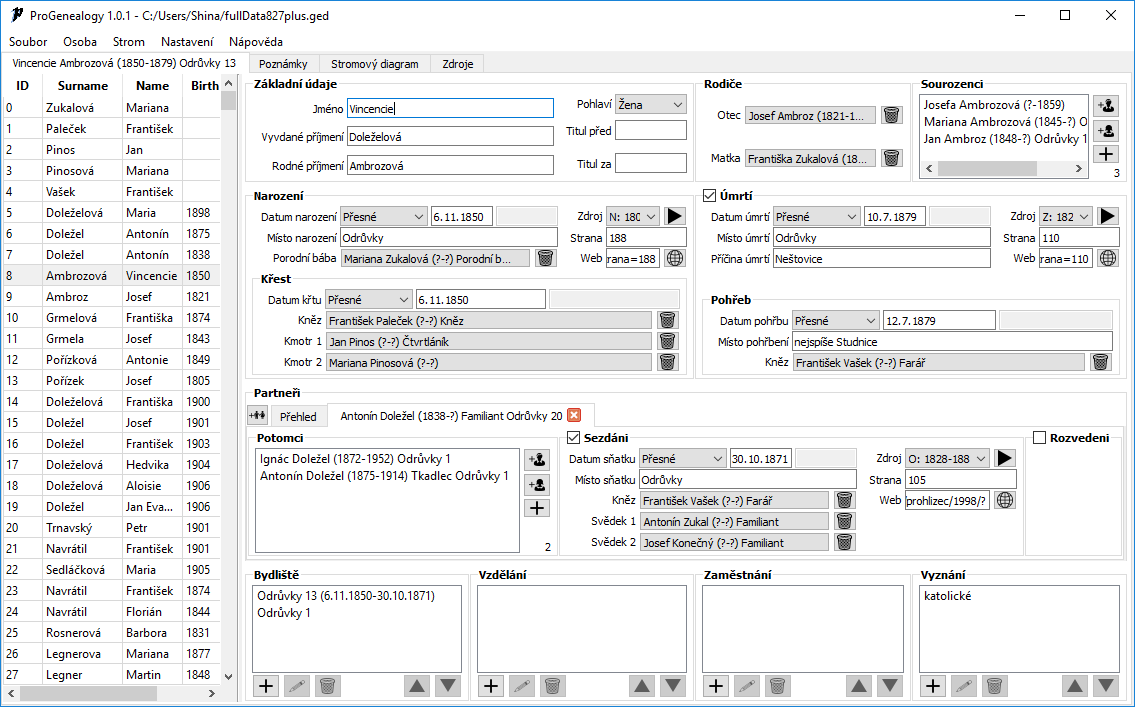
\includegraphics[width=15cm]{implem/indi.png}
			\caption{Rozhraní pro výběr a~editaci osoby}
			\label{fig:implemIndi}
		\end{figure}
		V~levé části obrazovky je seřaditelný seznam všech evidovaných osob. V~pravé části okna jsou potom rozloženy detailní informace o~vybrané osobě. Zobrazení se skládá ze čtyř vertikálně rozmístěných oddílů, které obsahují logicky související data.\par
		První z~oddílů se nachází v~horní části zobrazení podrobností o~osobě. Obsahuje v~sobě základní údaje o~osobě a~její nejbližší pokrevní rodině, tedy jméno a~příjmení osoby, její rodiče a~sourozence.\par
		Pod tímto oddílem se nachází boxy definující základní životní události osoby. Obsahují informace o~narození a~křtu i~data o~případném úmrtí a~pohřbu.\par
		V~dalším bloku se nachází informace o~případných partnerstvích sledované osoby a~o~jejích potomcích. U~partnerů mohou být dodatečné informace o~tom, zda byla dvojice sezdána nebo zda došlo k~rozvodu.\par
		Poslední blok slouží k~evidenci dodatečných informací. Je zde možné zachytit vývoj bydliště, vzdělání, zaměstnání a~náboženského vyznání osoby v~čase. Jednotlivé záznamy je možné libovolně řadit a~upravovat.\par
		Hlavní inspirací pro tuto záložku byla hlavní obrazovka českého programu Ancestry, popsaného v~sekci~\ref{sec:ance}. Tato skutečnost je velmi dobře viditelná v~uspořádání komponent v~okně. Aplikace \emph{ProGenealogy} ale v~tomto prostoru přináší nová pole, která nabízí i~zaznamenání pokročilých informací o~křtu či pohřbu. Aplikace také umožňuje zobrazování potomků podle partnera a~používá oproti Ancestry upravený systém pro odkazování na osoby, např. rodiče.\par
		Dále aplikace umožňuje citování zdrojů. Prostor pro citace je u~záznamů o~narození úmrtí a~sňatku. Zdroje z~dané oblasti odpovídající zadanému časovému horizontu jsou zobrazeny v~poli se seznamem, z~něhož uživatel může vybrat vhodný zdroj pro citování a~doplnit informace týkající se citované strany. Pro urychlení přístupu ke zdroji uživatel může citaci doplnit o~odkaz na webovou stránku s~digitalizovaným zdrojem.\par
	
		\subsection*{Výsledný vzhled rozhraní pro zobrazení stromu}
		Další důležitou část zobrazení tvoří plocha pro vykreslení stromového diagramu. Vzhled rozhraní aplikace, přepnuté do této záložky, je ilustrován v~obrázku~\ref{fig:implemTree}.\par
		\begin{figure}[h]
			\centering
			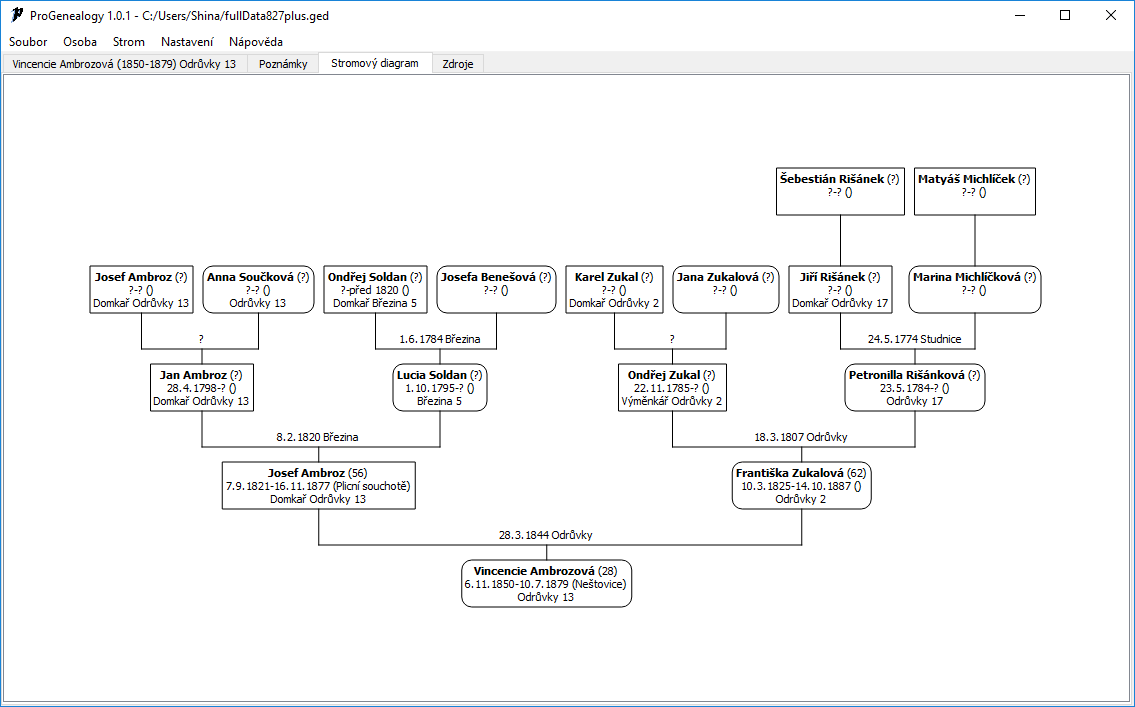
\includegraphics[width=15cm]{implem/tree.png}
			\caption{Rozhraní pro zobrazení stromu}
			\label{fig:implemTree}
		\end{figure}
		Vykreslení diagramu je voláno skrze nabídku v~menu \uv{Strom}. Zde si uživatel může zvolit typ diagramu pro vykreslení a~výsledný diagram také exportovat. Náhled exportovaného stromu je k~dispozici v~obrázku~\ref{fig:implemOutlet}. Jedná se o~vývod z~předků osoby jménem Vincencie Ambrozová exportovaný do formátu pdf. \par
		Aktuálně je v~programu k~dispozici pět typů diagramů~--~vývod z~předků, agnátní a~kognátní vývod, rozrod rodu a~strom příbuzenstva. Ty se po volbě vykreslí do prostoru scény ve sledované záložce.\par
		Diagram lze posouvat táhnutím myší nebo použitím posuvníků. Dvojitým poklepání myší na vybranou osobu se zobrazení přepne na podrobnosti o~vybrané osobě. Tato skutečnost umožňuje alternativní a~přehlednější způsob orientace ve vytvářeném rodokmenu. \par
		Obsahy buněk a~popisky u~sňatků je možné upravit skrze dialog v~nabídce \uv{Nastavení}. Úprava obsahu buněk stromu může být provedena jak po stránce obsahové, tak i~co se týče jejich formátování.\par
		\begin{figure}[h]
			\centering
			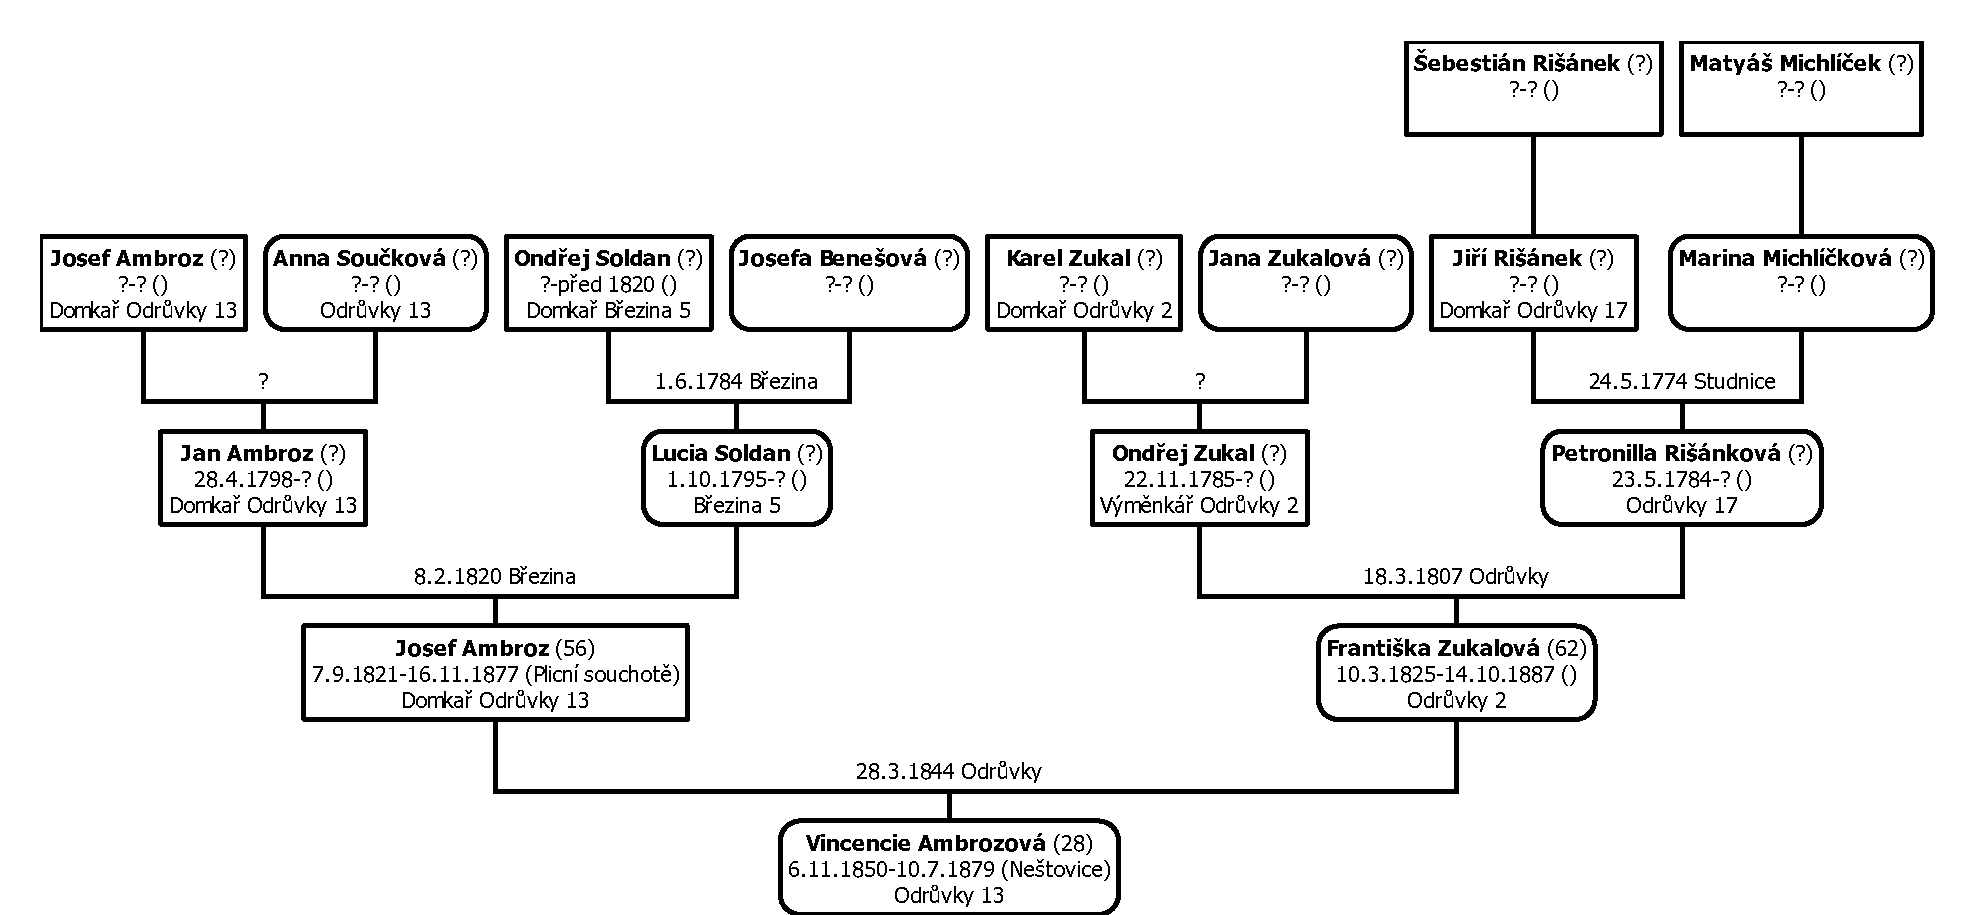
\includegraphics[width=15cm]{implem/vyvod.pdf}
			\caption{Diagram \uv{Vývod z~předků} exportovaný z~programu}
			\label{fig:implemOutlet}
		\end{figure}
		
		\subsection*{Výsledný vzhled rozhraní pro správu zdrojů}
		Poslední klíčovou součástí uživatelského rozhraní je obrazovka pro správu zdrojů. analogicky jako obrazovka vykreslující osoby sestává ze dvou sloupců. V~prvním z~nich je dostupný seznam všech evidovaných zdrojů. Ten je možné filtrovat skrze editaci textového pole nad ním.\par
		V~pravé straně obrazovky se již nacházejí detaily vybraného zdroje. V~horní sekci je možné vyplnit obecné informace o~zdroji jako celku, následují tři sekce, které evidují informace o~zápisech ve zdroji, které pokrývají jednotlivé životní události osob.\par
		Zdroje, které jsou v~této části programu evidovány, mohou být citovány u~událostí jednotlivých osob. Záznamy také slouží jako přehled pro uživatele, který díky nim může rychle navázat na pátrání v~dříve prozkoumané matrice. \par
		Tuto skutečnost zprostředkovávají možnosti záznamu stránek, na nichž se nachází zápisy jednotlivých obcí či typů záznamů. Díky nim se uživatel ve zdroji rychle zorientuje a~nemusí v~matriční knize opakovaně vyhledávat hranice jednotlivých oddílů. Nápomocný může být v~tomto ohledu také odkaz na digitalizovaný zdroj, který započetí pátrání ještě o~něco zrychluje a~zjednodušuje. \par
		\begin{figure}[H]
			\centering
			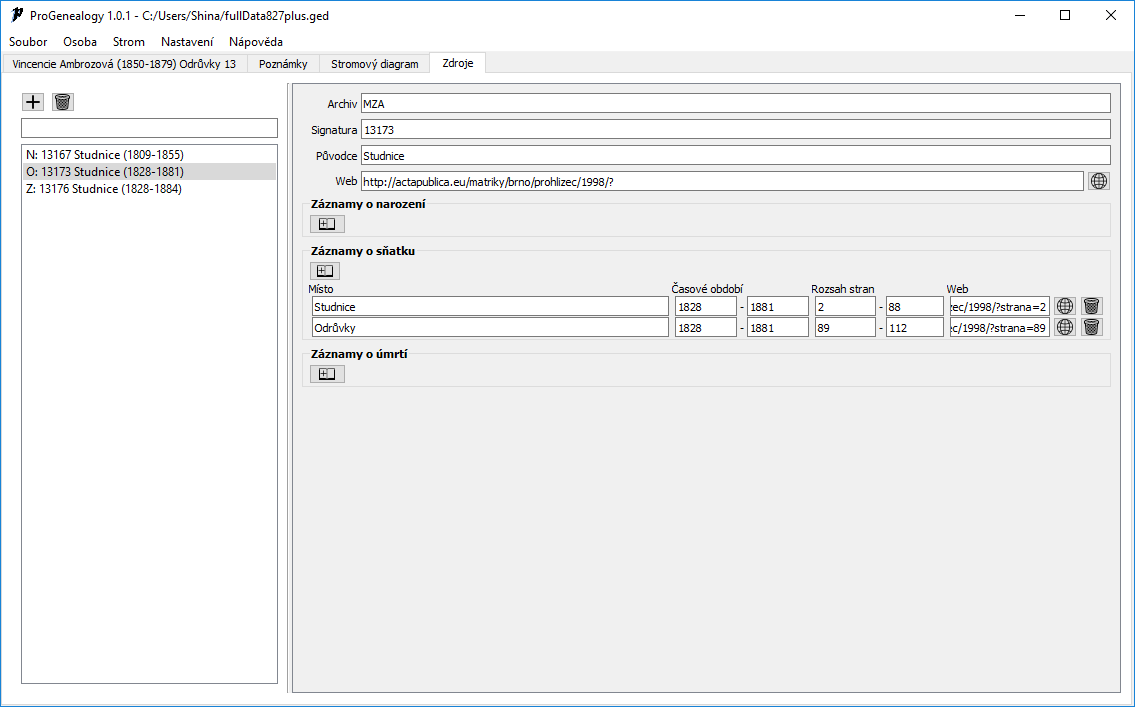
\includegraphics[width=15cm]{implem/src.png}
			\caption{Rozhraní pro přehled a~editaci zdrojů}
			\label{fig:implemSrc}
		\end{figure}

	
	\section{Metriky kódu}
	Práce na projektu byla započata dne 8. srpna 2018 a~ukončena dne 1. května 2019. Implementovaný kód je rozmístěn do celkem 319 zdrojových souborů. Je složen ze 23 234 neprázdných řádků, implementujících 13 738 výrazů. Kód obsahuje 11\% řádků s~komentáři.\par
	Aplikace funguje díky spolupráci 178 definovaných tříd. 135 z~nich jsou třídy implementující grafické uživatelské rozhraní. Jedna třída obsahuje v~průměru téměř deset metod. Každá metoda je potom implementována průměrně pěti výrazy. V~rámci celého projektu je naimplementováno pět funkcí. \par
	
	\begin{center}
		\begin{tabular}{||l|S[table-format=6.2]||}
			\hline
			%Datum vytvoření        & 8. 8. 2018 \\
			Počet souborů          & 319 \\
			Počet řádků            & 23 234 \\
			Počet výrazů           & 13 738 \\
			Řádky s~komentáři [\%] & 11 \\
			Počet definic tříd     &  178 \\
			Počet metod na třídu   & 9.81 \\
			Počet výrazů na metodu & 5.1 \\
			Počet funkcí           & 5 \\
			\hline
		\end{tabular}
	\end{center}


%===============================================================================
% Testování aplikace
%===============================================================================

\chapter{Testování aplikace}
\label{chap:test}
Testování je důležitou součástí životního cyklu každé aplikace. Nejinak tomu bylo i~v~případě aplikace vznikající v~rámci této práce. \par
Jelikož závěrečnou fází testování mělo být vypuštění aplikace mezi uživatele z~řad genealogů, muselo proběhnout důkladné testování programu. Bylo totiž klíčové, aby se program na uživatelských počítačích choval dle specifikace a~byl stabilní.\par
Proces testování probíhal v~několika etapách. Způsob testování se přitom lišil na základě fáze vývoje, v~níž se program nacházel. \par 

	\section*{Automatické testy jádra aplikace}
	Během vývoje jádra aplikace nebylo možné využít pro účely testování uživatelské rozhraní. Aby bylo potvrzeno, že implementace metod odpovídá specifikaci rozhraní, bylo vytvořeno několik automatických testovacích případů. \par
	První testovací případ se pokouší o~import souboru a~kontroluje, zda import proběhl v~pořádku. Další případ porovnává počet naimportovaných struktur proti očekávanému počtu struktur. Dále je provedena kontrola, zda mají konkrétní data očekávané hodnoty. Zkontrolována je takto vybraná osoba i~záznam o~zdroji. Poslední testovací případ porovnává hodnoty struktury pro evidenci data s~očekávanými hodnotami.\par
	Pro tvorbu testovacího projektu a~implementaci testovacích případů byl použit framework Qt Test~\cite{bib:QtTest}. Tento framework slouží k~vytváření automatických testů aplikací založených na Qt. Kromě provolávání metod a~kontroly jejich výsledků umožňuje prostřednictvím simulování interakcí z~klávesnice a~myši testovat i~uživatelské rozhraní.\par
		
	\section*{Manuální testování uživatelského rozhraní aplikace}
	Testování uživatelského rozhraní probíhalo dle potřeby manuálně. Tvorba automatických testů byla zavrhnuta, protože byla v~rozporu s~dynamickým vývojem aplikace, kdy docházelo k~častým zásahům do struktury rozhraní a~automatické testy by tedy nebyly trvanlivé.\par
	Po dokončení implementace každé funkcionality proběhly její manuální testy ve spuštěném uživatelském rozhraní. Identifikované chyby byly přímo opravovány.\par
	Další aspekt manuálního testování se zaměřoval na uživatelskou přívětivost aplikace. Spočíval ve spolupráci s~budoucími uživateli. Uživatel dostal sadu úkolů, které měl v~programu provést. Jeho interakce s~aplikací byla podrobena pozorování a~poté byla od uživatele získána zpětná vazba. Na základě získaných postřehů potom byly identifikovány slabé stránky rozhraní a~byly provedeny kroky směřující k~jejich vylepšení.\par
	
	
	\section*{Testování alfa verze aplikace}
	Alfa verze aplikace byla dokončena 23. dubna 2019. Aplikace byla označena jako \emph{ProGenealogy 1.0.0}. Cílem alfa verze bylo otestovat funkčnost aplikace na různých verzích systému Windows a~odhalit kritické chyby, s~nimiž by se uživatelé při používáni aplikace mohli setkat. Na testování alfa verze se podíleli čtyři uživatelé. Ani jeden z~nich nepocházel z~genealogické komunity.\par
	Testování proběhlo manuálně na počítačích se systémy Windows 7 Home Premium, Windows 7 Professional a~Windows 10 Home s~lokalizací v~českém jazyce. Poslední stroj používal operační systém Windows 10 Education s~lokalizací v~anglickém jazyce. \par
	Cíleně byl pozorován jazyk, v~němž se aplikace zobrazí při prvním spuštění. Tento jazyk by se měl odvíjet od jazyka prostředí, kde je program spuštěn. Bylo nutné, aby tento požadavek program splňoval, jelikož spuštění programu v~angličtině by uživatele odlákalo. Testováním bylo potvrzeno, že se aplikace spouští v~odpovídajícím jazyce.\par
	Aplikace byla všemi testujícími potvrzena jako stabilní program. Za běhu aplikace nebyly testujícími uživateli identifikovány žádné problémy, které by vedly k~jejímu předčasnému ukončování. \par
	Během dalšího testování bylo objeveno celkem čtrnáct chyb a~navrhnuto pět zlepšení. Byl identifikován problém, vedoucí k~nevhodnému rozložení obrazovky pro osobu a~zdroje při prvním spuštění aplikace. Tato fatální chyba způsobovala, že byly skryty součásti rozhraní sloužící pro editaci podrobností v~obrazovce s~osobou a~se zdrojem. Bylo také zjištěno, že aplikace povoluje definování cyklických vztahů mezi osobami. Poslední kritická chyba souvisela s~konfigurovatelnými popisky osob. Pokud byly dosazované hodnoty příliš dlouhé, mohla tato skutečnost vést k~nechtěnému zvětšení okna aplikace za hranice obrazovky. \par
	\begin{figure}[b!]
		\centering
		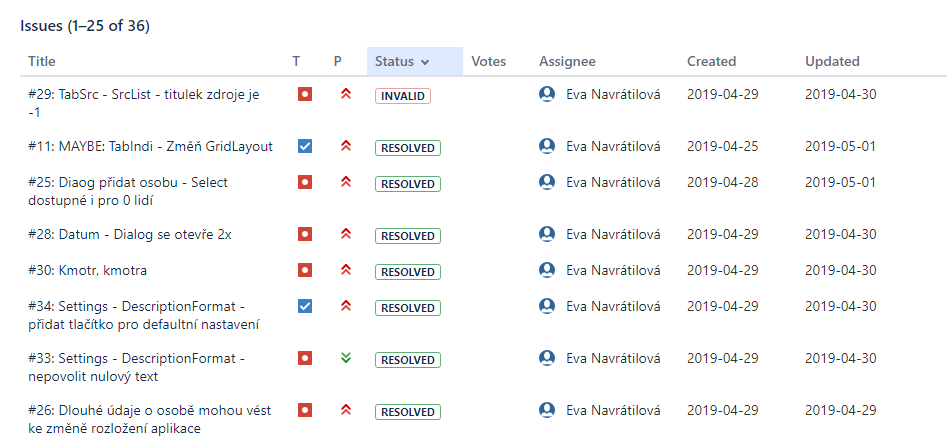
\includegraphics[width=15cm]{test/issueTracker.png}
		\caption{Výčet problémů v~alfa verzi evidovaný v~produktu Bitbucket}
		\label{fig:issueTrack}
	\end{figure}
	Nahlášené chyby byly zaznamenávány prostřednictvím služby Atlassian Bitbucket ve veřejném systému správy problémů. Náhled části zaznamenaných problémů, objevených v~alfa verzi, je k~dispozici v~obrázku~\ref{fig:issueTrack}. Po opravení chyb a~implementaci navržených rozšíření vznikla beta verze programu.\par
	
	\section*{Testování beta verze aplikace}
	Beta verze aplikace s~označením \emph{ProGenealogy 1.0.1} byla vytvořena 1. května 2019. Téhož dne byla zpřístupněna skupině uživatelů z~řad českých a~slovenských genealogů.\par
	Komunikace s~uživateli probíhala skrze Facebookovou stránku aplikace. Byly vytvořeny dva příspěvky. První z~nich odkazoval na stažení aplikace, druhý z~nich byl složen z~obrázků demonstrujících práci s~aplikací a~její možnosti. Tento příspěvek je k~nahlédnutí v~obrázku~\ref{fig:fb}. Oba tyto příspěvky byly dále sdíleny ve skupině Genealogie CZ+SK, sdružující české a~slovenské genealogy.\par
	Příspěvek s~odkazem na stažení programu oslovil ke dni 16. května 2019 1 569 lidí, z~nichž 743 o~příspěvek projevilo zájem. Snímky, zobrazující práci s~aplikací oslovily k~témuž datu celkem 1 880 uživatelů Facebooku, přičemž zájem o~příspěvek projevilo 1 333 z~nich.\par
	\begin{figure}[h!]
		\centering
		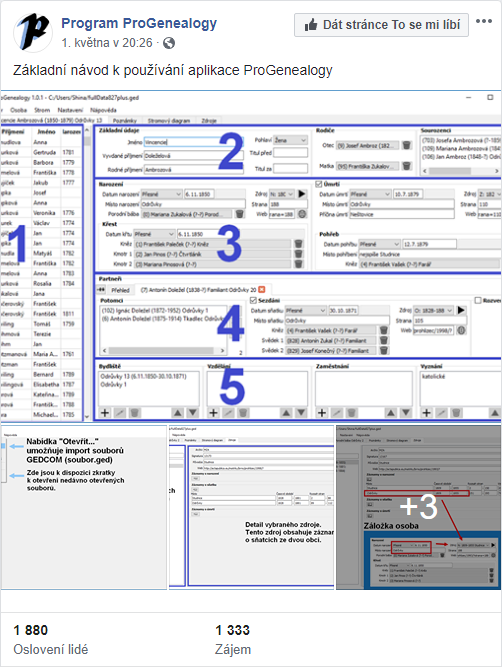
\includegraphics[width=9cm]{test/fb.png}
		\caption{Facebookový příspěvek s~obrázkovým návodem k~používání programu}
		\label{fig:fb}
	\end{figure}
	Uživatelé byli v~rámci těchto příspěvků požádání o~vyzkoušení aplikace a~poskytnutí zpětné vazby. Ta byla předávána prostřednictvím Facebookových komentářů a~zpráv, ale především skrze speciální hodnotící formulář.\par
	
	
	\section{Hodnocení aplikace uživateli z~řad genealogů}
	Zpětná vazba k~aplikaci probíhala především prostřednictvím hodnotícího formuláře. Plné znění dotazníku je k~nahlédnutí v~příloze~\ref{append:formHodnoceni}. Ve formuláři hodnotili respondenti ovládání aplikace, navrhovali vylepšení a~vytýkali zpozorované problémy.\par
	Dotazník vyplnilo ke dni 16. května 2019 třicet šest respondentů, kteří otestovali beta verzi aplikace. Jedna odpověď přitom byla samotným svým autorem označena za duplicitní, proto byla sloučena s~předchozí autorovou odpovědí a~vyřazena z~porovnávání. V~následujících odstavcích tedy bude hodnoceno pouze zbylých 35 jedinečných odpovědí.\par
	Více než 70~\% respondentů strávilo testováním aplikace více než třicet minut, přičemž většina z~této skupiny testování věnovala mezi půl hodinou a~hodinou.\par
	
	% Dojmy z aplikace
	První otázka týkající se aplikace se zaměřovala na dojmy, které v~uživatelích program zanechal. Jak je znázorněno v~diagramu~\ref{chart:hodnoDojmy}, většina respondentů hodnotila aplikaci jako celek pozitivně. Dvacet šest respondentů se vyjádřilo kladně, šest respondentů mělo smíšené dojmy a~tři hodnotili program jako celek negativně.\par
	\begin{figure}[bh!]
		\begin{tikzpicture}
			\pie [rotate = 180] {74.3/Pozitivní, 17.1/Smíšené, 8.6/Negativní}
		\end{tikzpicture}
		\caption{Dojmy uživatelů z~beta verze aplikace}
		\label{chart:hodnoDojmy}
	\end{figure}
	Respondenti oceňovali přizpůsobení pro české prostředí, jednoduchý, čistý a~moderní vzhled, přehlednost i~jednoduchost ovládání. Negativní aspekty hodnocení vycházely často z~nepochopení uživatelského rozhraní. Do budoucna tedy bude potřeba rozhraní upravit tak, aby byly tyto případy ještě sníženy. Uživatelé se zrakovými potížemi si stěžovali na nemožnost nastavení velikosti písma v~programu. \par
	Za zmínku jistě stojí i~skutečnost, že více než čtvrtina respondentů ve svých hodnoceních výslovně zmínila, že oceňují skutečnost, že jsou všechny záznamy umístěny na jediné obrazovce. Oproti tomu pouze jeden z~dotázaných uvedl, že přestože chápe účel, má ohledně této skutečnosti rozporuplné pocity, a~další respondent přímo uvedl, že mu toto rozložení nevyhovuje. Je tedy zřejmé, že tyto výsledky hrají výrazně ve prospěch zachování aktuálního rozložení, doplněného o~případné drobnější úpravy.\par
	
	% Jak se vám aplikace ovládala?
	Respondenti byli dále požádáni, aby ohodnotili ovládání aplikace, a~to na stupnici od jedné do šesti, přičemž jednička vyjadřuje, že ovládání je výborné, šestka naopak špatné ovládání. Výsledné hodnocení respondenty je shrnuto v~diagramu~\ref{chart:hodnoOvla}.\par
	Většina respondentů aplikaci ohodnotila jako průměrně dobře ovladatelnou, přičemž druhé nejčastější hodnocení se přiklánělo dokonce k~možnosti vyjadřující výbornou ovladatelnost. V~kladné polovině spektra se dohromady pohybovalo téměř 90~\% hodnocení. Většinově kladné názory podporuje i~průměrná hodnota ve výši téměř 2.3 na stupnici od jedné do šesti. \par
	
	\pgfplotstableread[row sep=\\,col sep=&]{
    values & ovladani & prechod \\
    1      & 25.7     & 20      \\
    2      & 42.9     & 42.9    \\
    3      & 20       & 17.1    \\
    4      & 5.7      & 5.7     \\
    5      & 0        & 11.4    \\
    6      & 5.7      & 2.9     \\
    }\hodnoSest
	
	\begin{figure}[h]
		\begin{tikzpicture}
			\begin{axis}[
					ybar,
					symbolic x coords={1,2,3,4,5,6},
					xtick=data,
					nodes near coords,
					ymin=0,ymax=50,
					ylabel={\%},
				]
				\addplot table[x=values,y=ovladani]{\hodnoSest};
			\end{axis}
		\end{tikzpicture}
		\caption{Hodnocení aplikace z~hlediska ovládání}
		\label{chart:hodnoOvla}
	\end{figure}
	
	Jelikož je aplikace svým rozhraním podobná českému programu Ancestry, předpokládalo se, že dosavadní uživatelé tohoto programu budou aplikaci hodnotit pozitivněji než zbytek respondentů. Tato hypotéza se ovšem nepotvrdila, hodnocení uživatelů, kteří měli zkušenosti s~aplikací Ancestry, nebyli výrazně pozitivnější ani negativnější než hodnocení zbytku uživatelů. Tato skutečnost je velmi pozitivní. Vypovídá totiž o~tom, že grafické rozhraní aplikace je intuitivní i~pro uživatele, kteří se s~aplikací s~podobným rozhraním ještě nesetkali.\par
	
	% Byli byste ochotni přejít na aplikaci
	Další otázka se snažila zachytit ochotu uživatelů přejít z~aplikace, kterou aktuálně používají, na aplikaci \emph{ProGenealogy}. Získané výsledky jsou shrnuty v~diagramu~\ref{chart:hodnoPrechod}. Přestože se jednalo teprve o~beta verzi, vedla si aplikace poměrně dobře i~v~tomto ohledu. Většina uživatelů vyjádřila průměrnou ochotu přejít na tuto aplikaci. Vysokou ochotu vyjádřilo nad očekávání dokonce 20~\% respondentů. Možnost změny aplikace zvažovalo celkem 80~\% z~dotazovaných. Zbylí uživatelé prozatím o~změně spíše neuvažovali. \par
	\begin{figure}[h]
		\begin{tikzpicture}
			\begin{axis}[
					ybar,
					symbolic x coords={1,2,3,4,5,6},
					xtick=data,
					nodes near coords,
					ymin=0,ymax=50,
					ylabel={\%},
				]
				\addplot table[x=values,y=prechod]{\hodnoSest};
			\end{axis}
		\end{tikzpicture}
		\caption{Ochota uživatelů přejít na aplikaci \emph{ProGenealogy}}
		\label{chart:hodnoPrechod}
	\end{figure}
	
	% Co se líbilo
	Další otázka uživatele vyzvala, aby zmínili, co se jim na aplikaci líbilo. Ohlasy sklízela především jednoduchost, přehlednost a~intuitivnost rozhraní aplikace. Respondenti chválili také možnost konfigurovat obsah buněk v~diagramech a~možnosti zaznamenání podrobnějších informací o~osobě na jednom místě. Pozitivně byl hodnocen i~český původ aplikace a~její lokalizace do českého jazyka, která byla základním požadavkem.\par
	
	% Co by změnili
	Respondenti byli dále tázáni, jaké změny by v~současné podobě aplikace provedli. Nejčastější výtky směřovaly k~pomalému importu dat. Ten plyne ze skutečnosti, že před samotným importem probíhá přepis identifikátorů na reprezentaci, která odpovídá definici identifikátorů tak, jak jsou chápány v~programu. Tento přepis zabírá u~dat s~počtem osob pohybujícím se v~řádech tisíců dlouhou dobu.\par
	Zbytek návrhů popisoval celou řadu nápadů, co upravit. Žádná z~připomínek se ale neopakovala, nejednalo se tedy o~obecně sdílené názory. Čtyři respondenti, tedy 11~\% ze všech dotazovaných uvedlo, že žádné změny nejsou třeba.\par
		
	% Co by přidali
	Požadavky na přidání funkcionalit se naopak ukázaly jako obecně sdílené. 31~\% dotázaných by stálo o~zavedení správy obrázků. 20~\% respondentů uvedlo, že si přejí rozšířit možnosti vykreslování stromu a~přidat možnost vyhledávání mezi osobami. 11.4~\% respondentů si přálo obohatit program o~textové výstupy u~jednotlivých osob a~o~rodokmenové statistiky.\par
	
	% Co by odebrali
	Více než 40~\% uživatelů uvedlo, že za zbytečnou nepovažují žádnou součást programu, načež dalších 17~\% uživatelů uvedlo, že si žádné zbytečné komponenty nejsou vědomi. Výraznější kritiku sklidila pouze kolonka pro vyvdané příjmení, 11~\% uživatelů by si přálo tuto část z~formuláře odstranit. Jednotliví respondenti potom upozorňovali na různé části uživatelského rozhraní, které by si do budoucna zasloužily úpravy.\par
	
	% Zhodnocení
	Výsledky výzkumu mezi uživateli jsou pro další vývoj programu velmi přínosné. Přestože byla aplikace převážnou částí respondentů hodnocena pozitivně, je zřejmé, že aby získala svoje místo mezi zavedenými programy, bude třeba ji obohatit o~celou řadu funkcionalit. \par
	Velmi žádaná je podpora multimediálních souborů v~podobě obrázků. Zájem je mezi uživateli také o~vylepšené vykreslování rodových diagramů.\par
	Jako klíčový krok ke zlepšení aplikace bylo ale jednoznačně identifikováno zrychlení načítání velkých souborů. Pomalé načítání komplikovalo používání beta verze programu s~velkými daty a~byl to nejpalčivější problém, který byl v~aplikaci identifikován.\par
	Tento problém již byl adresován a~došlo k~jeho opravě. Program nyní zvládá načtení velkých dat v~řádek vteřin až minut oproti předchozí bilanci pohybující se v~řádech desítek minut až hodin.\par
	

%===============================================================================
% Závěr
%===============================================================================

\chapter{Závěr}

Cílem práce bylo navrhnout, implementovat a otestovat aplikaci pro interaktivní vytváření rodokmenů. V~teoretické části této práce byly definovány genealogické pojmy a~popsány existující genealogické aplikace. Byla zhodnocena přívětivost jejich uživatelského rozhraní a~rozsah jejich funkcionality. \par
Dále byl proveden průzkum mezi respondenty z~řad českých a~slovenských genealogů, týkající se používaných genealogických aplikací. Výsledky průzkumu byly analyzovány a~na jejich základě byla vytvořena specifikace požadavků.\par
Na základě specifikace požadavků byl proveden návrh aplikace. Aplikace byla rozdělena do dvou vrstev. První vrstva zapouzdřuje jádro aplikace a~zprostředkovává rozhraní k~importu a~exportu dat a~k~přístupu k~samotným záznamům. Druhá vrstva potom definuje uživatelské rozhraní a~jeho komponenty.\par
Navrhnutý program byl implementován v~jazyce C++ za využití frameworku Qt. Práce byla též formou plakátu prezentována na konferenci Excel@FIT, kde získala od veřejnosti 19~bodů. \par
Po vytvoření beta verze programu proběhlo testování mezi uživateli z~řad českých a~slovenských genealogů. Aplikace sklidila mezi uživateli převážně pozitivní ohlasy. Byla oceňována její přehlednost, intuitivnost a~umístění souvisejících komponent v~jedné obrazovce.  \par
Na základě ohlasů uživatelů, kteří program otestovali, byly provedeny jeho další úpravy. Dále byly na základě jejich zpětné vazby vyhodnoceny návrhy na zlepšení, které by mohly pomoci určit další směr vývoje aplikace.\par
Velmi žádaná je mezi uživateli podpora obrázků v~aplikaci. Velká část uživatelů také stojí o~rozšíření funkcionalit týkajících se vykreslování grafických výstupů. Zájem byl projeven také o~obohacení programu o~statistické funkce a~textové výstupy z~rodokmenu. Aplikaci by také bylo vhodné doplnit o~možnost automatických aktualizací, která by zjednodušila distribuci nových verzí.\par

%===============================================================================

  
  % Kompilace po částech (viz výše, nutno odkomentovat)
  % Compilation piecewise (see above, it is necessary to uncomment it)
  %\subfile{projekt-01-uvod-introduction}
  % ...
  %\subfile{chapters/projekt-05-conclusion}


  % Pouzita literatura / Bibliography
  % ----------------------------------------------
\ifslovak
  \makeatletter
  \def\@openbib@code{\addcontentsline{toc}{chapter}{Literatúra}}
  \makeatother
  \bibliographystyle{bib-styles/slovakiso}
\else
  \ifczech
    \makeatletter
    \def\@openbib@code{\addcontentsline{toc}{chapter}{Literatura}}
    \makeatother
    \bibliographystyle{bib-styles/czechiso}
  \else 
    \makeatletter
    \def\@openbib@code{\addcontentsline{toc}{chapter}{Bibliography}}
    \makeatother
    \bibliographystyle{bib-styles/englishiso}
  %  \bibliographystyle{alpha}
  \fi
\fi
  \begin{flushleft}
  \bibliography{projekt-20-literatura-bibliography}
  \end{flushleft}

  % vynechani stranky v oboustrannem rezimu
  % Skip the page in the two-sided mode
  \iftwoside
    \cleardoublepage
  \fi

  % Prilohy / Appendices
  % ---------------------------------------------
  \appendix
\ifczech
  \renewcommand{\appendixpagename}{Přílohy}
  \renewcommand{\appendixtocname}{Přílohy}
  \renewcommand{\appendixname}{Příloha}
\fi
\ifslovak
  \renewcommand{\appendixpagename}{Prílohy}
  \renewcommand{\appendixtocname}{Prílohy}
  \renewcommand{\appendixname}{Príloha}
\fi
%  \appendixpage

% vynechani stranky v oboustrannem rezimu
% Skip the page in the two-sided mode
%\iftwoside
%  \cleardoublepage
%\fi
  
\ifslovak
%  \section*{Zoznam príloh}
%  \addcontentsline{toc}{section}{Zoznam príloh}
\else
  \ifczech
%    \section*{Seznam příloh}
%    \addcontentsline{toc}{section}{Seznam příloh}
  \else
%    \section*{List of Appendices}
%    \addcontentsline{toc}{section}{List of Appendices}
  \fi
\fi
  \startcontents[chapters]
  \setlength{\parskip}{0pt}
  % seznam příloh / list of appendices
  % \printcontents[chapters]{l}{0}{\setcounter{tocdepth}{2}}
  
  \ifODSAZ
    \setlength{\parskip}{0.5\bigskipamount}
  \else
    \setlength{\parskip}{0pt}
  \fi
  
  % vynechani stranky v oboustrannem rezimu
  \iftwoside
    \cleardoublepage
  \fi
  
  % Přílohy / Appendices
  %===============================================================================
% Autorka: Bc. Eva Navrátilová
% Kontakt: xnavra54@stud.fit.vutbr.cz, navratie@gmail.com
%===============================================================================

% Tento soubor nahraďte vlastním souborem s přílohami (nadpisy níže jsou pouze pro příklad)
% This file should be replaced with your file with an appendices (headings below are examples only)

% Umístění obsahu paměťového média do příloh je vhodné konzultovat s vedoucím
% Placing of table of contents of the memory media here should be consulted with a supervisor
%\chapter{Obsah přiloženého paměťového média}

%\chapter{Manuál}

%\chapter{Konfigurační soubor} % Configuration file

\chapter{Obsah přiloženého paměťového média}
	\label{append:cd}
	\begin{itemize}
		\item \texttt{readme.txt}~--~Obsahuje informace o~aplikaci, instalaci a~repozitáři
		\item \texttt{doc/}
		\begin{itemize}
			\item \texttt{thesis/}~--~Text této práce a~latexové zdrojové kódy
			\item \texttt{doxygen/}~--~Dokumentace kódu vygenerovaná prostřednictvím Doxygenu
			\item \texttt{tutorial/}~--~Obrázkový návod k~použití aplikace
		\end{itemize}
		\item \texttt{src/}~--~Makefile
		\begin{itemize}
			\item \texttt{src/}~--~Zdrojové kódy aplikace a~knihoven třetích stran
			\begin{itemize}
				\item \texttt{3rd-party/}~--~Zdrojové kódy použitých externích knihoven
				\item \texttt{kernel/}~--~Zdrojové kódy jádra aplikace
				\item \texttt{userinterface/}~--~Zdrojové kódy uživateslkého rozhraní aplikace
				\item \texttt{language/}~--~Překlady aplikace do přiřozených jazyků
			\end{itemize}
			\item \texttt{test/}~--~Zdrojové kódy automatických testů aplikace
		\end{itemize}
		\item \texttt{bin/}~--~Binární soubory
		\begin{itemize}
			%\item \texttt{linux/}~--~Spustitelný soubor pro linux (generuje se příkazem \texttt{make} v~\texttt{src/})
			\item \texttt{windows/}~--~Spustitelný .exe soubor pro Windows
		\end{itemize}
	\end{itemize}


\chapter{Plakát} % poster
\newpage
\label{append:poster}
\begin{figure}[H]
	\centering
	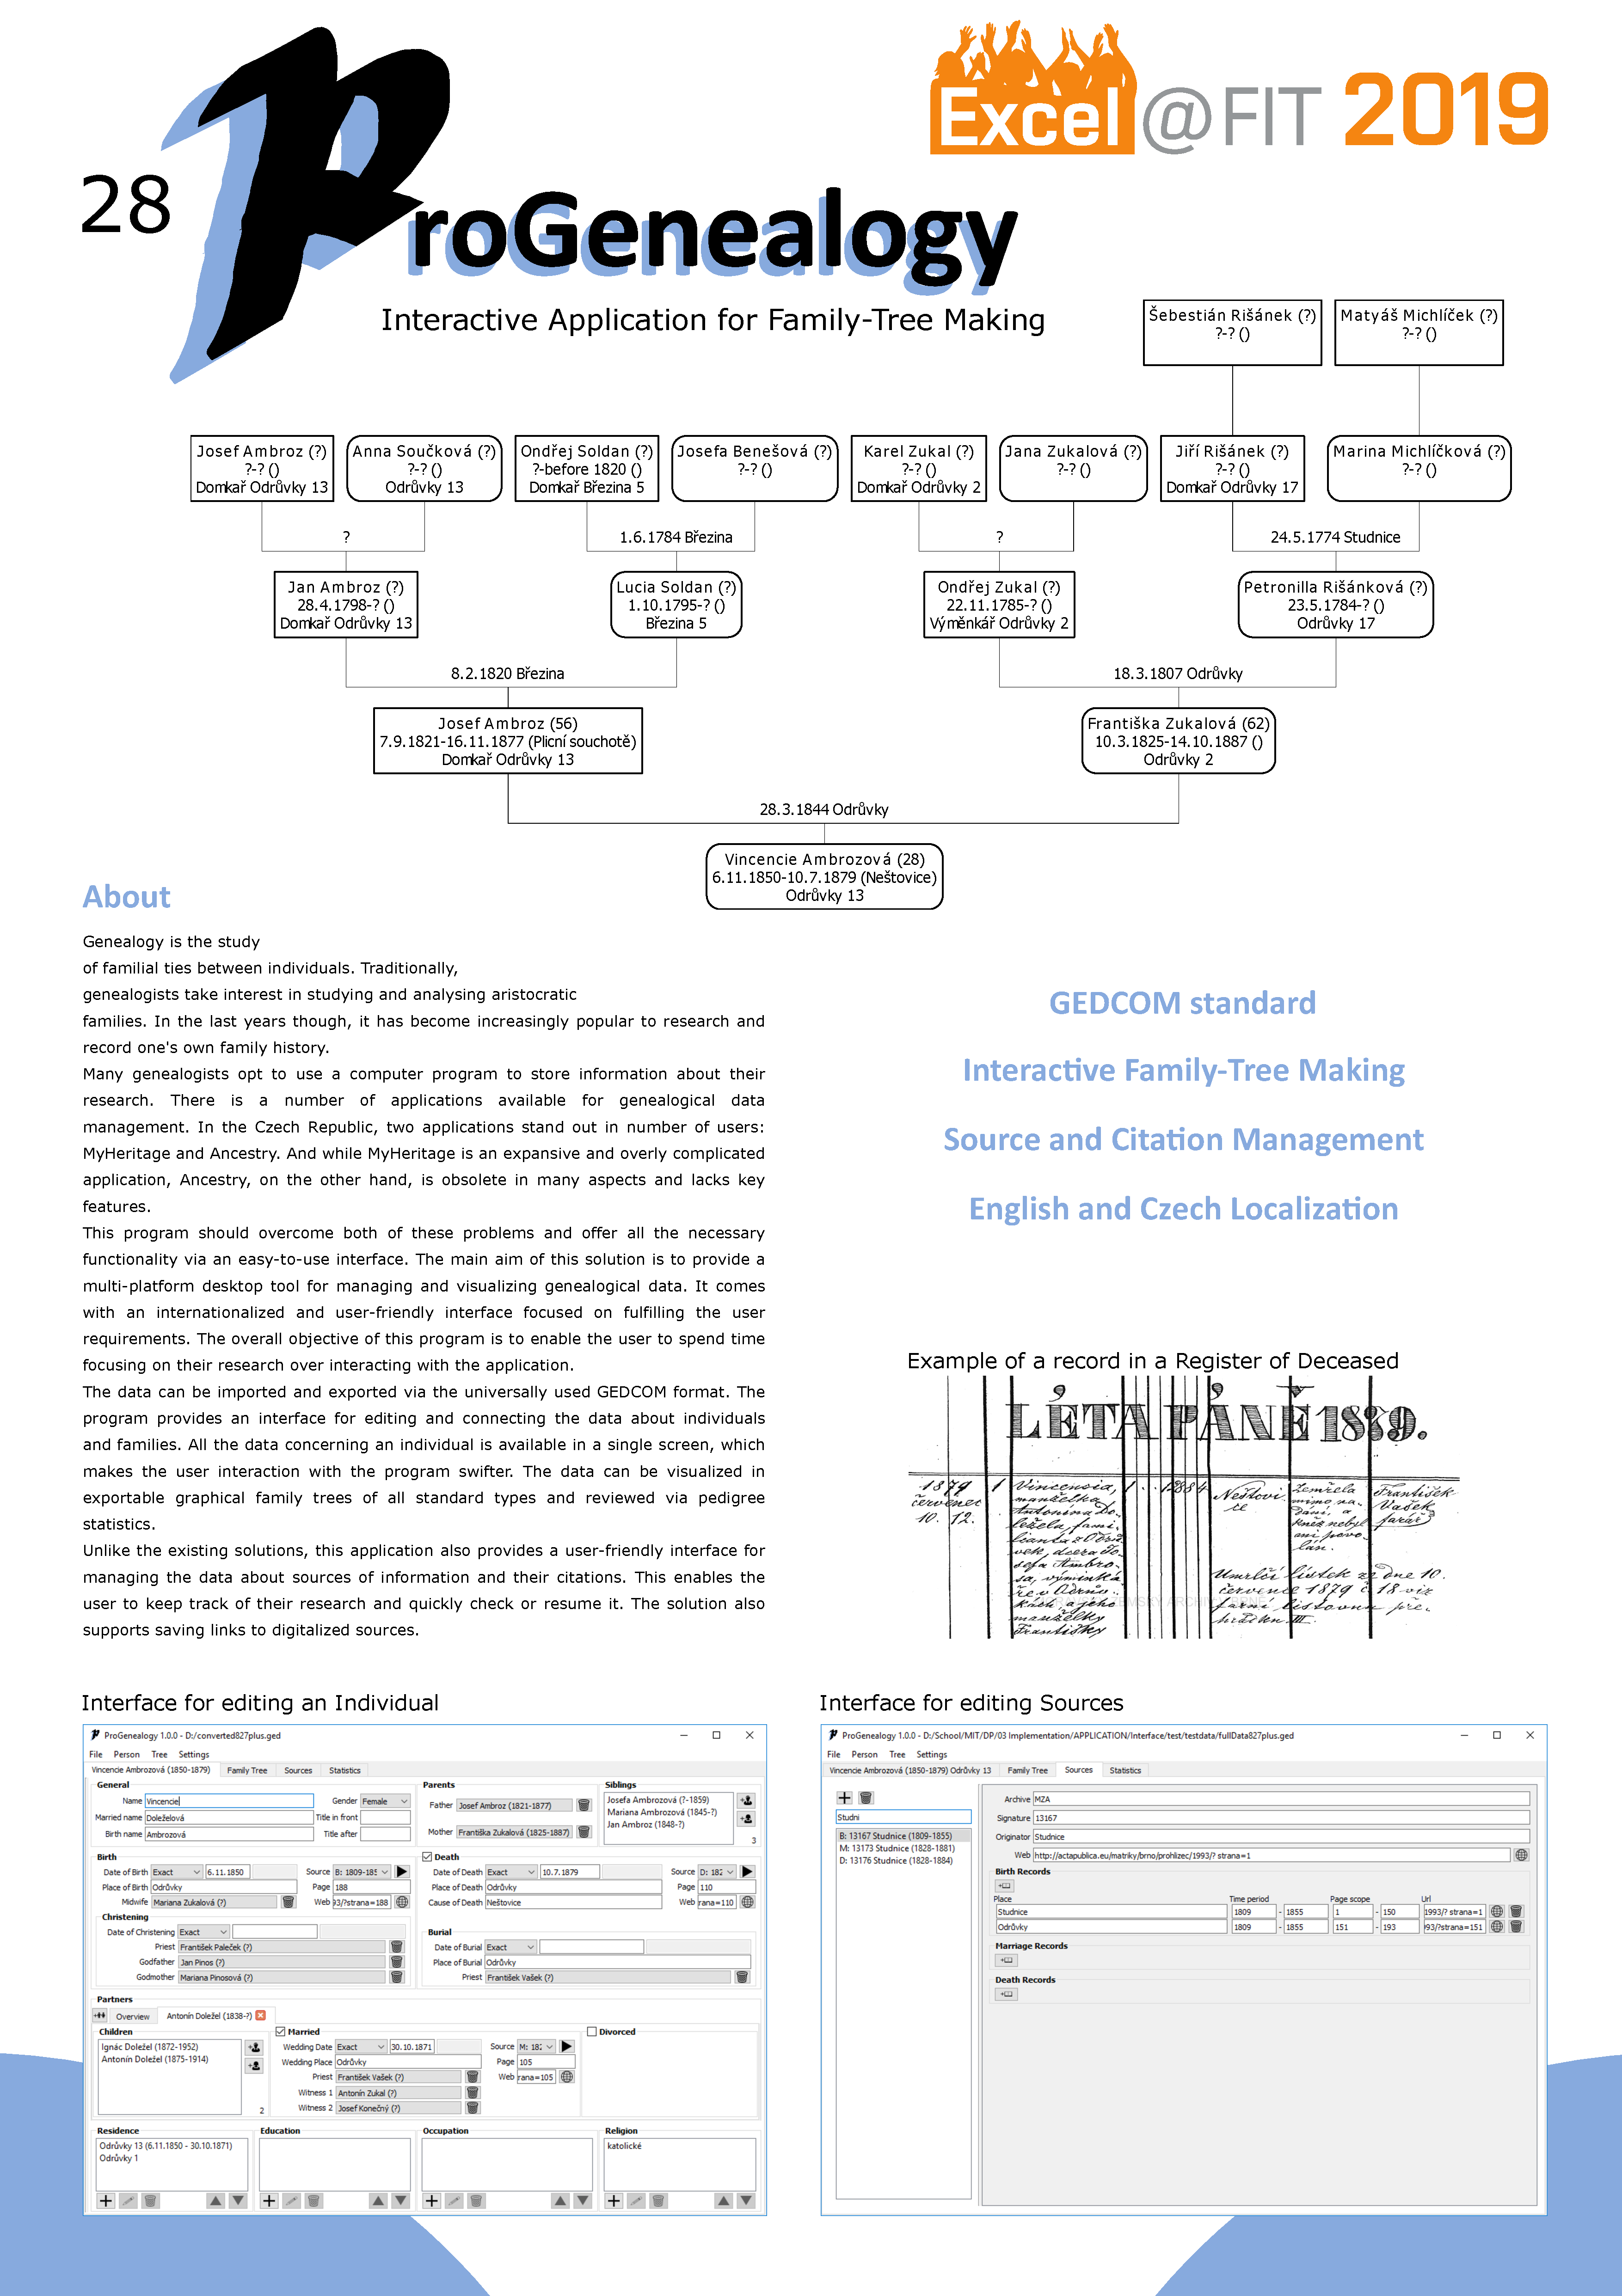
\includegraphics[width=15cm]{28_poster.pdf}
	\caption{Plakát využitý při účasti na konfercenci Excel@FIT}
\end{figure}


\chapter{Diagram tříd jádra aplikace}
\label{append:designKernel}
\begin{figure}[H]
	\centering
	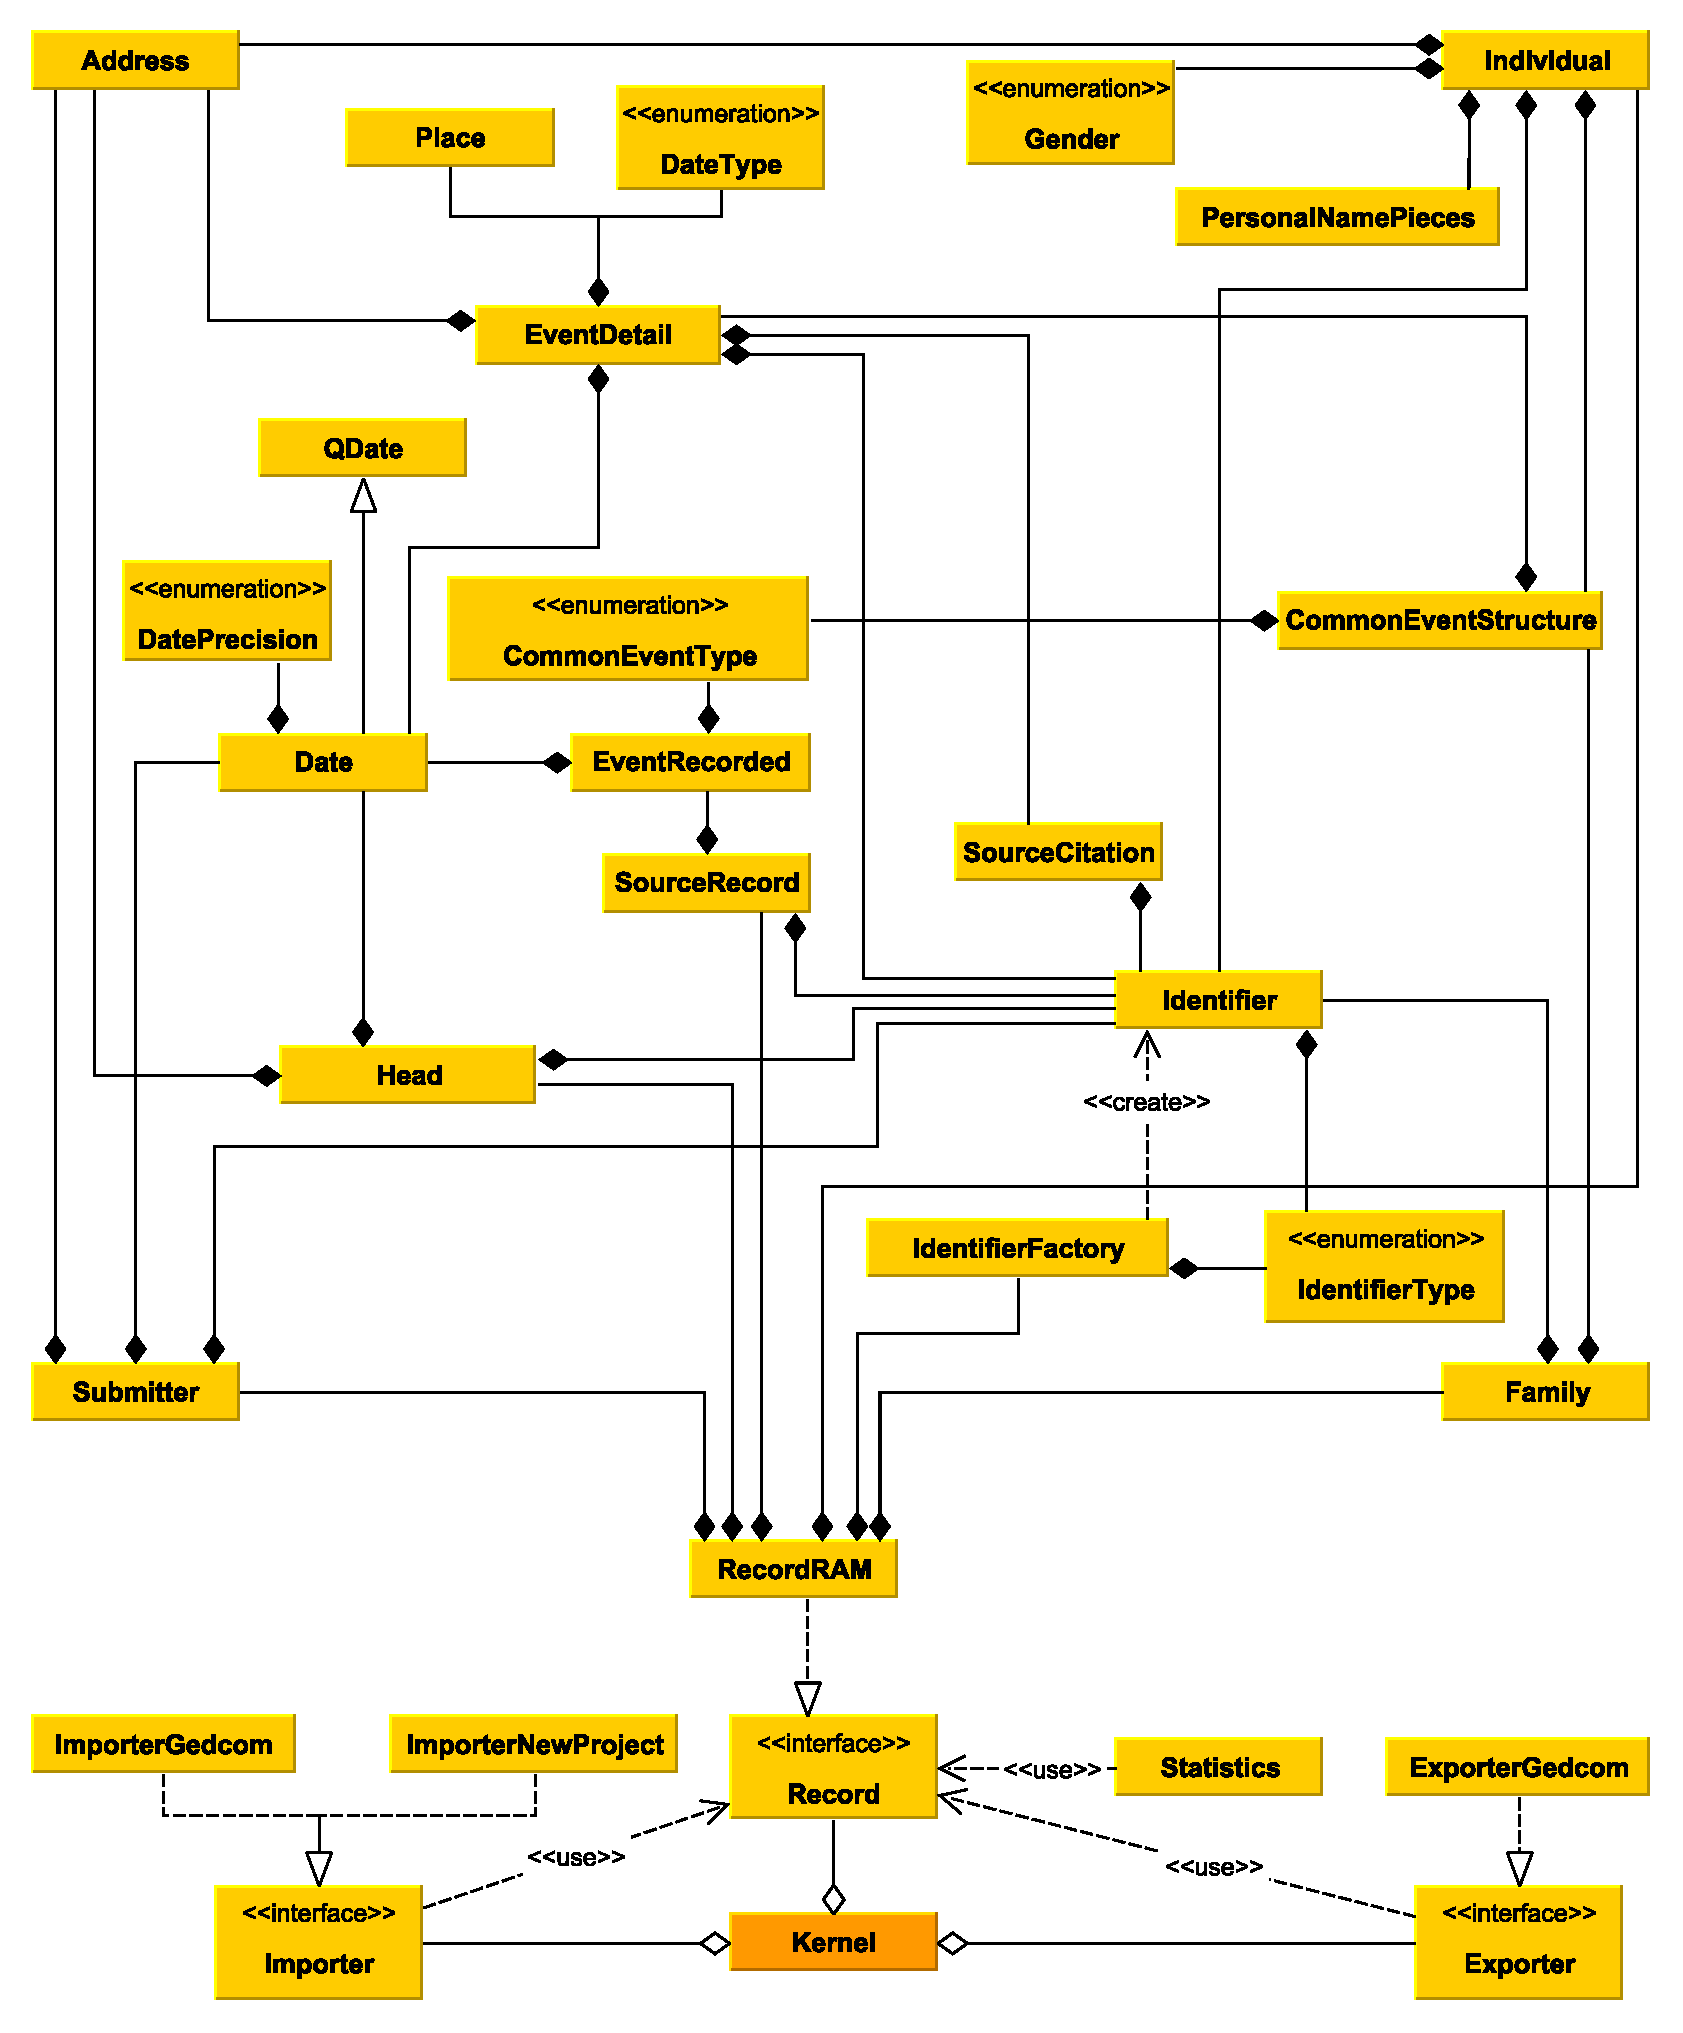
\includegraphics[width=13cm]{design/programFullClassOnly.pdf}
	\caption{Diagram tříd jádra aplikace}
\end{figure}




\chapter{Vzory formulářů}
	\section{Zkušenosti s genealogickými aplikacemi}
		\label{append:formZkusenosti}
		\subsection*{Jak dlouho pracujete s genealogickými programy?}
		\begin{itemize}
			\item[$\circ$] Méně než rok
			\item[$\circ$] 1 až 2 roky
			\item[$\circ$] 2 až 6 let
			\item[$\circ$] více než 6 let
		\end{itemize}
		\subsection*{Jaký genealogický program aktuálně používáte?}
		\dotfill
		\subsection*{Proč jste si tento program vybrali?}
		\dotfill
		\subsection*{Co vám na programu vyhovuje?}
		\dotfill
		\subsection*{Co vám v programu chybí, co byste na něm změnili?}
		\dotfill
		\subsection*{Zaznamenáváte u osob zdroje informací?}
		\begin{itemize}
			\item[$\circ$] Vždy
			\item[$\circ$] Občas
			\item[$\circ$] Nikdy
		\end{itemize}
		\subsection*{Jakým způsobem zdroje informací ukládáte do programu?}
		\begin{itemize}
			\item[$\square$] Webový odkaz na digitalizovanou stránku matriky, kde se nachází záznam o předkovi
			\item[$\square$] Signatura matriky, číslo stránky
			\item[$\square$] Zaznamenávám i pozici zápisu na stránce
			\item[$\square$] \dotfill
		\end{itemize}
		\subsection*{Vaše poznámky}
		\dotfill

	\newpage
	\section{Hodnocení aplikace ProGenealogy}
		\label{append:formHodnoceni}
		\subsection*{Jakou aplikaci aktuálně používáte?}
		\begin{itemize}
			\item[$\square$] MyHeritage (Webové rozhraní)
			\item[$\square$] Ancestry
			\item[$\square$] MyHeritage FamilyTreeBuilder
			\item[$\square$] \dotfill
		\end{itemize}
		\subsection*{Jaké jsou vaše dojmy z aplikace ProGenealogy?}
		\dotfill
		\subsection*{Jak se vám aplikace ovládala?}
		Výborně    \quad $\circ$ $\circ$ $\circ$ $\circ$ $\circ$ $\circ$ \quad Špatně
		\subsection*{Uvažovali byste o přechodu na tuto aplikaci?}
		Určitě ano \quad $\circ$ $\circ$ $\circ$ $\circ$ $\circ$ $\circ$ \quad Určitě ne
		\subsection*{Co se vám na aplikaci líbí?}
		\dotfill
		\subsection*{Co byste na aplikaci změnili?}
		\dotfill
		\subsection*{Co vám v aplikaci chybí? Co byste přidali?}
		\dotfill
		\subsection*{Co bylo v aplikaci zbytečné? Co byste odebrali?}
		\dotfill
		\subsection*{Jak dlouho jste s aplikací ProGenealogy pracovali?}
		\begin{itemize}
			\item[$\circ$] méně než 10 minut
			\item[$\circ$] 10 až 30 minut
			\item[$\circ$] 30 minut až 1 hodinu
			\item[$\circ$] více než 1 hodinu
		\end{itemize}
	
	




  
  % Kompilace po částech (viz výše, nutno odkomentovat)
  % Compilation piecewise (see above, it is necessary to uncomment it)
  %\subfile{projekt-30-prilohy-appendices}
  
\end{document}
